%%%%%%%%%%%%%%%%%%%%%%%%%%%%%%%%%%%%%%%%%
% MHL Thesis LaTeX Template
% Version 1.1 (09/09/2021)
%
% This template is based on a template by:
% Steve Gunn (http://users.ecs.soton.ac.uk/srg/softwaretools/document/templates/)
% Sunil Patel (http://www.sunilpatel.co.uk/thesis-template/)
%
% found on:
% http://www.LaTeXTemplates.com/template/masters-doctoral-thesis
%
% Template license:
% CC BY-NC-SA 3.0 (http://creativecommons.org/licenses/by-nc-sa/3.0/)
%%%%%%%%%%%%%%%%%%%%%%%%%%%%%%%%%%%%%%%%%

%----------------------------------------------------------------------------------------
%	DOCUMENT CONFIGURATIONS
%----------------------------------------------------------------------------------------
\PassOptionsToPackage{greek,main=english}{babel}
\documentclass[
	12pt, % The default document font size, options: 10pt, 11pt, 12pt
	% oneside, % Two side (alternating margins) for binding by default, uncomment to switch to one side
	twoside,
	english,
	onehalfspacing, % Single line spacing, alternatives: singlespacing or doublespacing
	%draft, % Uncomment to enable draft mode (no pictures, no links, overfull hboxes indicated)
	%nolistspacing, % If the document is onehalfspacing or doublespacing, uncomment this to set spacing in lists to single
	liststotoc, % Uncomment to add the list of figures/tables/etc to the table of contents
	toctotoc, % Uncomment to add the main table of contents to the table of contents
	parskip, % Uncomment to add space between paragraphs
	%nohyperref, % Uncomment to not load the hyperref package
	headsepline, % Uncomment to get a line under the header
	chapterinoneline, % Uncomment to place the chapter title next to the number on one line
	% consistentlayout, % Uncomment to change the layout of the declaration, abstract and acknowledgements pages to match the default layout
]{MastersDoctoralThesis} % The class file specifying the document structure

%----------------------------------------------------------------------------------------
%	PACKAGES
%----------------------------------------------------------------------------------------

\usepackage[utf8]{inputenc} % Required for inputting international characters
\usepackage[LGR, T1]{fontenc} % Output font encoding for international characters
\usepackage{mathpazo} % Use the Palatino font by default
\usepackage[backend=biber,style=numeric,natbib=true,sorting=none]{biblatex} % Use the bibtex backend with the numeric citation style
\usepackage[autostyle=true]{csquotes} % Required to generate language-dependent quotes in the bibliography
\usepackage[section]{placeins}
\usepackage{float}
\usepackage{comment}
\usepackage{algorithm}
\usepackage[noend]{algpseudocode}
\usepackage{hyperref}
\usepackage{graphicx}
\usepackage{subcaption}
\usepackage{amsmath}
\usepackage{algpseudocode}



\makeatletter
\makeatother
\def\infinity{\rotatebox{90}{8}}
\addtocontents{loa}{\def\string\figurename{Algorithm}}

%----------------------------------------------------------------------------------------
%	BIBLIOGRAPHY FILES
%----------------------------------------------------------------------------------------

% Todo: comment out example.bib file when done reading the template instructions
% \addbibresource{example.bib} % The filename of the bibliography
\addbibresource{references.bib} % The filename of the bibliography

%----------------------------------------------------------------------------------------
%	MARGIN SETTINGS
%----------------------------------------------------------------------------------------

\geometry{
	paper=a4paper, % Change to letterpaper for US letter
	inner=2.5cm, % Inner margin
	outer=3.8cm, % Outer margin
	bindingoffset=.5cm, % Binding offset
	top=1.5cm, % Top margin
	bottom=1.5cm, % Bottom margin
	% showframe, % Uncomment to show how the type block is set on the page
}

%----------------------------------------------------------------------------------------
%	THESIS INFORMATION
%----------------------------------------------------------------------------------------

% Todo: fill info below
\thesistitle{Interactive User Environment Application on Kubernetes} % Your thesis title, this is used in the title and abstract, print it elsewhere with \ttitle
\author{Kyriakos \textsc{Chalvatzis}} % Your name, this is used in the title page and abstract, print it elsewhere with \authorname
\supervisor{Prof.Vasilis \textsc{Samoladas}} % Your supervisor's name, this is used in the title page, print it elsewhere with \supname
\degree{Electrical and Computer Engineer} % Your degree name, this is used in the title page and abstract, print it elsewhere with \degreename
\subject{Electrical and Computer Engineering} % Your subject area, this is not currently used anywhere in the template, print it elsewhere with \subjectname
\keywords{Diploma Thesis} % Keywords for your thesis, this is not currently used anywhere in the template, print it elsewhere with \keywordnames
\university{\href{https://www.tuc.gr/}{Technical University of Crete}} % Your university's name and URL, this is used in the title page and abstract, print it elsewhere with \univname
\department{\href{https://www.ece.tuc.gr/}{School of Electrical and Computer Engineering}} % Your department's name and URL, this is used in the title page and abstract, print it elsewhere with \deptname
% \group{\href{https://www.mhl.tuc.gr/}{Microprocessor and Hardware Laboratory}} % Your research group's name and URL, this is used in the title page, print it elsewhere with \groupname
\faculty{
		% \href{http://faculty.university.com}{Faculty Name}
} % Your faculty's name and URL, this is used in the title page and abstract, print it elsewhere with \facname

\AtBeginDocument{
	\hypersetup{pdftitle=\ttitle} % Set the PDF's title to your title
	\hypersetup{pdfauthor=\authorname} % Set the PDF's author to your name
	\hypersetup{pdfkeywords=\keywordnames} % Set the PDF's keywords to your keywords
}

%----------------------------------------------------------------------------------------
%	TITLE PAGE
%----------------------------------------------------------------------------------------

\begin{document}

\frontmatter % Use roman page numbering style (i, ii, iii, iv...) for the pre-content pages

\pagestyle{plain} % Default to the plain heading style until the thesis style is called for the body content

\begin{titlepage}
	\begin{center}
		{\scshape\LARGE \univname\par}
		\vspace{0.5cm} % University name
		\textsc{\Large Diploma Thesis}\\[0.5cm] % Thesis type

		\HRule\\[0.4cm] % Horizontal line
		{\huge \bfseries \ttitle\par}\vspace{0.4cm} % Thesis title

		\begin{minipage}[t]{0.4\textwidth}
			\begin{flushleft} \large
				\emph{Author:}\\
				% Todo: fill correct link
				\href{http://example.com/}{\authorname} % Author name - remove the \href bracket to remove the link
			\end{flushleft}
		\end{minipage}
		\begin{minipage}[t]{0.5\textwidth}
			\begin{flushright} \large
				\emph{Thesis Committee:} \\
				% Todo: fill correct link
				\href{https://www.ece.tuc.gr/el/index.php?id=4109&tx_tuclabspersonnel_list%5Bperson%5D=361&tx_tuclabspersonnel_list%5Baction%5D=person&tx_tuclabspersonnel_list%5Bcontroller%5D=List}{\supname}\\ % chktex 15 % Supervisor name - remove the \href bracket to remove the link
				% Todo: fill correct link, full name
				\href{https://www.ece.tuc.gr/el/i-scholi/prosopiko/single-display-person?tx_tuclabspersonnel_pi3%5Bpersonid%5D=771&cHash=7632eaf07b3963f9d990de818bdbcda9}{Prof. Nikolaos \textsc{Giatrakos}}\\
				% Todo: fill correct link, full name
				\href{https://www.ece.tuc.gr/el/index.php?id=4109&tx_tuclabspersonnel_list%5Bperson%5D=353&tx_tuclabspersonnel_list%5Baction%5D=person&tx_tuclabspersonnel_list%5Bcontroller%5D=List}{Prof. Euripides \textsc{Petrakis}}
			\end{flushright}
		\end{minipage}\\[0.2cm]

		
\includegraphics[scale=0.21]{Images/TUC_logo.png} % University/department logo - uncomment to place it
		\\
		
		\vfill

		\large \textit{A thesis submitted in fulfillment of the requirements\\ for the diploma of \degreename}\\[0.3cm] % University requirement text
		\textit{in the}\\[0.4cm]
		% \deptname\\\groupname\\[2cm] % Research group name and department name
		\deptname\\[2cm] % Research group name and department name

		\vfill

		{\large \today}\\ % Date
		\vfill
	\end{center}
\end{titlepage}

%----------------------------------------------------------------------------------------
%	ABSTRACT PAGE English
%----------------------------------------------------------------------------------------

\begin{abstract}
	\addchaptertocentry{\abstractname} % Add the abstract to the table of contents
	% Todo: Add English Abstract
	The following thesis presents the design and implementation of a 
	user-oriented analytical computing system deployed on the Kubernetes 
	platform. The system draws inspiration from core Unix design principles, 
	particularly in file and directory permissions, user hiererchy and 
	authorization management.

	The central ambition is to ease the operational quality of life for 
	data analysts working with sizable or not datasets, while maintaining 
	strict access control and support for concurrent multi-user interactions. 
	Users can upload and share datasets, submit batch job into execution using 
	pre-integrated applications, such as DuckDB, Bash, Octave, Pandas and others. 
	Designed with modularity and extensibility in mind, the platform aims to 
	abstract the complexity of orchestration, achieves abstraction of resource 
	allocation and job scheduling, providing users with a seamless interface 
	for analytical workflows. Each job lives and dies in a sandboxed containerized 
	environment, ensuring reproducibility and isolation.

	The solution demonstrates the feasibility of delivering a lightweight, flexible platform 
	that leverages Kubernetes’ native scalability to manage user resources, data, and jobs 
	efficiently. It offers a pathway for democratizing access to powerful analytics tooling, 
	especially in research and educational contexts where ease of deployment and extensibility 
	are vital.
\end{abstract}

%----------------------------------------------------------------------------------------
%	ABSTRACT PAGE Greek
%----------------------------------------------------------------------------------------

\begin{abstract}
	\addchaptertocentry{\abstractname} % Add the abstract to the table of contents
	% Todo: Add Greek Abstract
    \selectlanguage{greek}
	Η παρούσα διπλωματική εργασία παρουσιάζει τον σχεδιασμό και την υλοποίηση 
	ενός υπολογιστικού συστήματος ανάλυσης δεδομένων προσανατολισμένου στον 
	χρήστη, το οποίο αναπτύσσεται στην πλατφόρμα \textlatin{Kubernetes}. 
	Το σύστημα αντλέι έμπνευση από τις θεμελιώδεις αρχές σχεδιασμού του 
	\textlatin{Unix}, ιδιαίετερα ως προς τα δικαιώματα αρχείων, την ιεραρχία 
	χρηστών και τη διαχείρηση εξουσιοδοτήσεων. Κεντρική φιλοδοξία αποτελεί η 
	βελτίωση της καθημερινής εμπειρίας των αναλυτών δεδομένων που εργάζονται 
	με μεγάλους και όχι όγκους δεδομένων, διατηρώντας παράλληλα αυστηρό έλεγχο 
	πρόσβασης και υποστήριξη για ταυτόχρονη αλληλεπίδραση πολλών χρηστών. 
	Οι χρήστες μπορούν να ανεβάζουν και να διαμοιράζονται σύνολα δεδομένων, 
	καθώς και να υποβάλλουν παρτίδες εργασιών προς εκτέλεση χρησιμοποιώντας 
	προενσωματωμένες εφαρφμογές, όπως \textlatin{DuckDB}, \textlatin{Bash}, 
	\textlatin{Octave}, \textlatin{Pandas} και άλλες. Με σχεδιασμό που δίνει
	έμφαση στην μοντελοποίηση και την επεκτασιμότητα, η πλατφόρμα στοχεύει 
	στην απόκρυψη της πολυπλοκότητας της ενορχήστρωσης, της διαχείρισης πόρων 
	και του χρονοπρογραμματισμού εργασιών, προσφέροντας στους χρήστες ένα 
	ενιαίο και εύχρηστο περιβάλλον για ροές εργασίας ανάλυσης δεδομένων. 
	Κάθε εργασία εκτελέιται και τερματίζεται μέσα σε απομονωμένο περιβάλλον, 
	διασφαλίζοντας της αναπαραγωγιμότητα και την απομόνωση. Η λύση καταδεικνύει 
	τη δυνατότητα δημιουργίας μιας ελαφριάς και ευέλικτης πλατφόρμας που αξιοποιεί 
	την εγγενή επεκτασιμότητα του \textlatin{Kubernetes} για την αποδοτική διαχείριση 
	των χρηστών, των δεδομένων και των εργασιών. Αποτελεί μια προσέγγιση που διευρυνεί
	την πρόσβαση σε ισχυρά εργαλεία ανάλυσης, ιδιαίτερα σε ερευνητικά και εκπαιδευτικά 
	περιβάλλοντα όπου η ευκολία ανάπτυξης και η δυνατότητα επέκτασης είναι καθοριστικής 
	σημασίας.
\end{abstract}

%----------------------------------------------------------------------------------------
%	ACKNOWLEDGEMENTS
%----------------------------------------------------------------------------------------

\begin{acknowledgements}
	\addchaptertocentry{\acknowledgementname} % Add the acknowledgements to the table of contents
	% Todo: Add Acknowledgements
	First and foremost, I would like to  express my deep respect and appriciation 
	towards my advisor, Professor Vasilis Samoladas. His precise guidance served 
	as a beacon of clarity and stability throughout the often chaotic process of 
	designing and developing an entire system independently.
	
	I am also deeply grateful for the unwavering support and patience shown by my 
	close friends and family, who stood by me selflessly and with enduring encouragement 
	during this demanding journey.

	Last but not least, I would like to extend my heartfelt thanks to the esteemed members 
	of the Thesis Committee, Professor E. Petrakis and Professor N. Giatrakos, as well as 
	to my fellow colleagues and students on campus who shared this experience.

	% I would like to acknowledge the use of OpenAI's ChatGPT, which assisted me throughout 
	% the thesis process — from refining ideas and structuring sections and rephrasing many 
	% aspects to improving language clarity and generating code examples. While all critical 
	% decisions, validations, and final wording were made by me, the AI served as a helpful 
	% companion during development and documentation and information digging.
\end{acknowledgements}

%----------------------------------------------------------------------------------------
%	LIST OF CONTENTS/FIGURES/TABLES PAGES
%----------------------------------------------------------------------------------------

\tableofcontents % Prints the main table of contents
\listoffigures % Prints the list of figures
\listoftables % Prints the list of tables
\listofalgorithms% Prints the list of algorithms
\addcontentsline{toc}{chapter}{List of Algorithms}

%----------------------------------------------------------------------------------------
%	ABBREVIATIONS
%----------------------------------------------------------------------------------------

% Todo: edit to your requirements
% spell-checker: disable
\begin{abbreviations}{ll} % Include a list of abbreviations (a table of two columns)]
	\textbf{API}	& \textbf{A}pplication \textbf{P}rogramming \textbf{I}nterface\\
	\textbf{CNS}	& \textbf{C}loud \textbf{N}ative \textbf{S}torage\\
	\textbf{CS}		& \textbf{C}omputer \textbf{S}cience\\
	\textbf{CRUD}	& \textbf{C}reate \textbf{R}ead \textbf{U}pdate \textbf{D}elete\\
	\textbf{CSS}	& \textbf{C}ascade \textbf{S}tyle \textbf{S}heets\\
	\textbf{CSV}	& \textbf{C}omma \textbf{S}eperated \textbf{V}alues\\
	\textbf{DAG}	& \textbf{D}irected \textbf{A}cyclic \textbf{G}raph\\
	\textbf{DSL}	& \textbf{D}omain \textbf{S}pecific \textbf{L}anguage\\
	\textbf{ETL}	& \textbf{E}xtract \textbf{T}ransform \textbf{L}oad\\
	\textbf{HTTP}	& \textbf{H}yper\textbf{T}ext \textbf{T}ransfer \textbf{P}rotocol\\
	\textbf{HTML}	& \textbf{H}yper\textbf{T}ext \textbf{M}arkup \textbf{L}anguange\\
	\textbf{I/O}	& \textbf{I}nput / \textbf{O}utput\\
	\textbf{JWKS}	& \textbf{J}SON \textbf{W}eb \textbf{K}ey \textbf{S}et\\
	\textbf{JWT}	& \textbf{J}son \textbf{W}eb \textbf{T}oken\\
	\textbf{JS}		& \textbf{J}ava\textbf{S}cript\\
	\textbf{JSON} 	& \textbf{J}ava\textbf{S}cript \textbf{O}bject \textbf{N}otation\\
	\textbf{K8S}	& \textbf{K}ubernete\textbf{S}\\
	\textbf{PaaS}	& \textbf{P}latform \textbf{a}s \textbf{a} \textbf{S}ervice\\
	\textbf{PV}		& Kubernetes \textbf{P}ersistent \textbf{V}olume\\
	\textbf{PVC}	& Kubernetes \textbf{P}ersistent \textbf{V}olume \textbf{C}laim\\
	\textbf{RBAC}	& \textbf{R}ole \textbf{B}ased \textbf{A}ccess \textbf{C}ontrol\\
	\textbf{S3}		& Amazon \textbf{S}imple \textbf{S}torage \textbf{S}ervice\\
	\textbf{SQL}	& \textbf{S}tructured \textbf{Q}uery \textbf{L}anguage\\
	\textbf{UID}	& \textbf{U}ser \textbf{ID}entification\\
	\textbf{GID}	& \textbf{G}roup \textbf{ID}entification\\
	\textbf{VID}	& \textbf{V}olume \textbf{ID}entification\\
	\textbf{RID}	& \textbf{R}esource \textbf{ID}entification\\
	\textbf{JID}	& \textbf{J}ob \textbf{ID}entification\\
\end{abbreviations}
% spell-checker: enable

%----------------------------------------------------------------------------------------
%	DEDICATION
%----------------------------------------------------------------------------------------

\dedicatory{Dedicated to my family and friends\ldots}

%----------------------------------------------------------------------------------------
%	THESIS CONTENT - CHAPTERS
%----------------------------------------------------------------------------------------

% Include the chapters of the thesis as separate files from the Chapters folder
% Uncomment the lines as you write the chapters
\pagestyle{thesis} % Return the page headers back to the "thesis" style
\mainmatter% Begin numeric (1,2,3...) page numbering

\chapter{Introduction}
\label{Chapter-Introduction}

\section{Purpose and Motivation}
\hspace{2mm}This project began as an effort to integrate a user-friendly `environment' layer into Kubernetes—an infrastructure known 
for its power and scalability, yet lacking direct support for user-centric entities. The goal was to make 
an environment where individual users can perform analytical computing in their own `space', especially enabling
data analysts to work with large-scale datasets, by abstracting the complexity of orchestration and container management.
As the system evolved, the focus deviated slightly towards a fully modular full stack platform that supports multiple users, secures
access with custom authentication, and enables storage provisioning, sharing, and execution of batch jobs using familiar tools such
as DuckDB, Bash, Octave, and Pandas~\cite{mckinney-proc-scipy-2010}. The motivation became to deliver a system 
that combines the robustness of cloud-native
technologies with the ease of use of desktop analytical environments—bridging the gap between DevOps infrastructure and 
end-user data workflows.

Ultimately, amongst some services, the bar was set to implement already existing enterprise level technology stacks to 
more basic and developer friendly as in ease of access and deployment versions. It had been a personal aspiration and 
challenge to create some utilities that are scoped for development with a laconic tone while maintaining inspiration by others.

\newpage

\section{Problem Statement}

\hspace{2mm}While modern data platforms such as Apache Airflow or Spark 
address large-scale, enterprise-level orchestration needs, they are often complex, heavyweight, and 
not designed with ease of use or modularity in mind—especially for individual analysts or smaller 
teams working on self-contained workflows.

This thesis does not seek to compete with such platforms, nor to introduce fundamentally new orchestration paradigms. 
Instead, it focuses on designing and implementing a lightweight, extensible system that simplifies the execution of batch 
data analysis jobs in a multi-user environment.

The core problem addressed is the absence of a simple, user-accessible platform where authenticated users can:
\begin{itemize}
    \item Upload datasets to a common, structured storage layer,
    \item Submit analytical jobs using containerized tools such as DuckDB, Pandas, or Octave,
    \item View job outputs and logs through a unified interface,
    \item And share or manage their data and jobs in a collaborative way.
\end{itemize}

This project presents a custom application built on top of Kubernetes~\cite{google-kubernetes} that abstracts away infrastructure complexity, 
offering a modular foundation upon which analytical tools can be plugged and executed in a reproducible, isolated manner. 
The overarching goal is to improve the user experience in running batch data workflows—not by reimagining distributed computation, 
but by making its power more accessible and flexible for real-world analysis tasks.



\section{Scope of the Project}
\hspace{2mm}The scope of this thesis includes the design, development, and integration of a modular microservice-based platform tailored to Kubernetes. 
The system introduces:

\begin{itemize}
    \item A custom authentication and user management service (\texttt{Minioth}).
    \item A central orchestration service (\texttt{Uspace}) that defines and manages user environments.
    \item A lightweight virtual filesystem abstraction (\texttt{Fslite}) for managing user data and metadata.
    \item Integration with MinIO for physical object storage.
    \item A WebSocket-enabled frontend service that provides real-time interaction and job monitoring capabilities.
\end{itemize}

The system supports uploading, sharing, and executing batch jobs using containerized tools, while abstracting the complexity of 
Kubernetes operations from the end user.

Out of scope for this project are scheduling algorithms, dynamic autoscaling and support for third-party 
authentication (e.g., OAuth~\cite{oauth2-rfc6749}).

The system is implemented in Go~\cite{golang}, a statically typed, compiled programming language designed for simplicity and concurrency.

The backend for the Services is implemented using the Gin web framework for Go~\cite{gingonic}, which provides performant HTTP routing and middleware integration.

\section{Thesis Contributions}
\hspace{2mm}The primary contributions of this thesis are as follows:
\begin{itemize}
    \item The design and implementation of a fully functional user-centric platform deployed on Kubernetes, 
    abstracting core orchestration mechanics from the user.
    \item A custom authentication service (\texttt{Minioth}) implementing user/group-based access control with secure 
    token issuance and verification.
    \item The \texttt{Uspace} service that defines and manages user environments, enabling secure job submission and resource 
    isolation.
    \item The \texttt{Fslite} abstraction layer that models user data and virtual resources in a hierarchical structure, 
    backed by object storage (MinIO).
    \item A WebSocket-integrated frontend allowing users to interactively monitor jobs and access 
    their workspace in real time.
    \item A demonstration of how Kubernetes-native resources and batch execution can be adapted to serve multi-user analytical 
    workflows in an accessible, extensible system.
\end{itemize}



\newpage
\section{Thesis Outline}
% Todo: Fill chapter descriptions
\begin{itemize}
    \item \textbf{Chapter 2 – Background and Theoretical Foundations:}  
    An overview of the core technologies and concepts underpinning the system, including Kubernetes, microservices, authentication models, 
    containerized workloads, and object storage.

    \item \textbf{Chapter 3 – Related Work:}  
    A review of existing platforms and tools related to data processing, user environment provisioning, and cloud-native architectures. 
    It highlights their limitations and positions this work within the broader landscape.

    \item \textbf{Chapter 4 – System Design and Architecture:}  
    The Architectural blueprint of the system, detailing the interactions between core services such as Minioth, Uspace, Fslite, and the Frontend. 
    The design goals of modularity, scalability, and security are emphasized.

    \item \textbf{Chapter 5 – System Usage \& Execution Flow:}  
    Describes how the system operates from both user and administrative perspectives. It details the deployment setup, system access points, 
    request-response structure, and error feedback mechanisms.  
    End-to-end workflows are illustrated through UI examples, including the job submission lifecycle.  

    \item \textbf{Chapter 6 – Evaluation and Robustness:}  
    An evaluation of the system’s behavior under various conditions, including performance, scalability, fault tolerance, and security. 
    Observations and informal benchmarks are included where applicable..

    \item \textbf{Chapter 7 – Conclusions and Future Work:}  
    Summarizes the work, reflects on its outcomes and limitations, and discusses potential directions for further development 
    and enhancement of the system.
\end{itemize}


\chapter{Background and Theoritical Foundations}
\label{Chapter-Background}

% Todo: Edit to your liking
\section{Kubernetes}

\begin{figure}[h!]
  \centering
  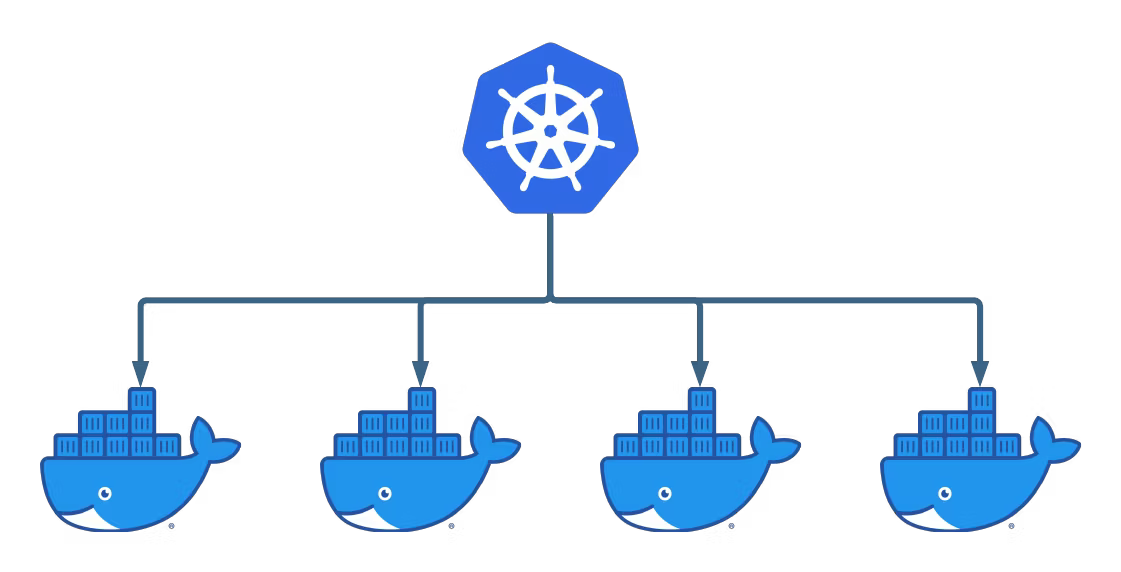
\includegraphics[width=1\textwidth]{Images/2024-04-10-k8s-vs-docker.png}
  \caption{Kubernetes}
  \label{fig:kubernetes}
\end{figure}

Kubernetes is an open-source container orchestration platform originally developed by Google~\cite{kubernetes-docs} 
and now maintained by the Cloud Native Computing Foundation (CNCF)~\cite{cncf-kubernetes}. It automates the deployment, 
scaling, and management of containerized applications across a cluster of machines. Kubernetes abstracts the infrastructure 
and provides primitives such as Pods, Deployments, Services, and Jobs, which allow developers to define complex systems 
declaratively.

% TODO more

In this project, Kubernetes serves as the core infrastructure layer for deploying isolated environments, managing job execution, 
and ensuring scalability and fault tolerance. The native support for namespaces, role-based access control (RBAC), and persistent 
volumes (PVs) makes it suitable for building multi-user platforms.
\section{Microservices}

The microservices architectural style structures an application as a collection of loosely coupled services, each responsible for 
a specific domain or capability~\cite{newman-microservices}. Microservices communicate primarily through lightweight mechanisms 
such as HTTP or messaging queues, and they are independently deployable.

This approach was adopted in the system to improve modularity and separation of concerns. For instance, authentication, job 
orchestration, and storage abstraction are implemented as separate services, allowing them to evolve independently and scale 
according to their individual loads.

\begin{figure}[h!]
  \centering
  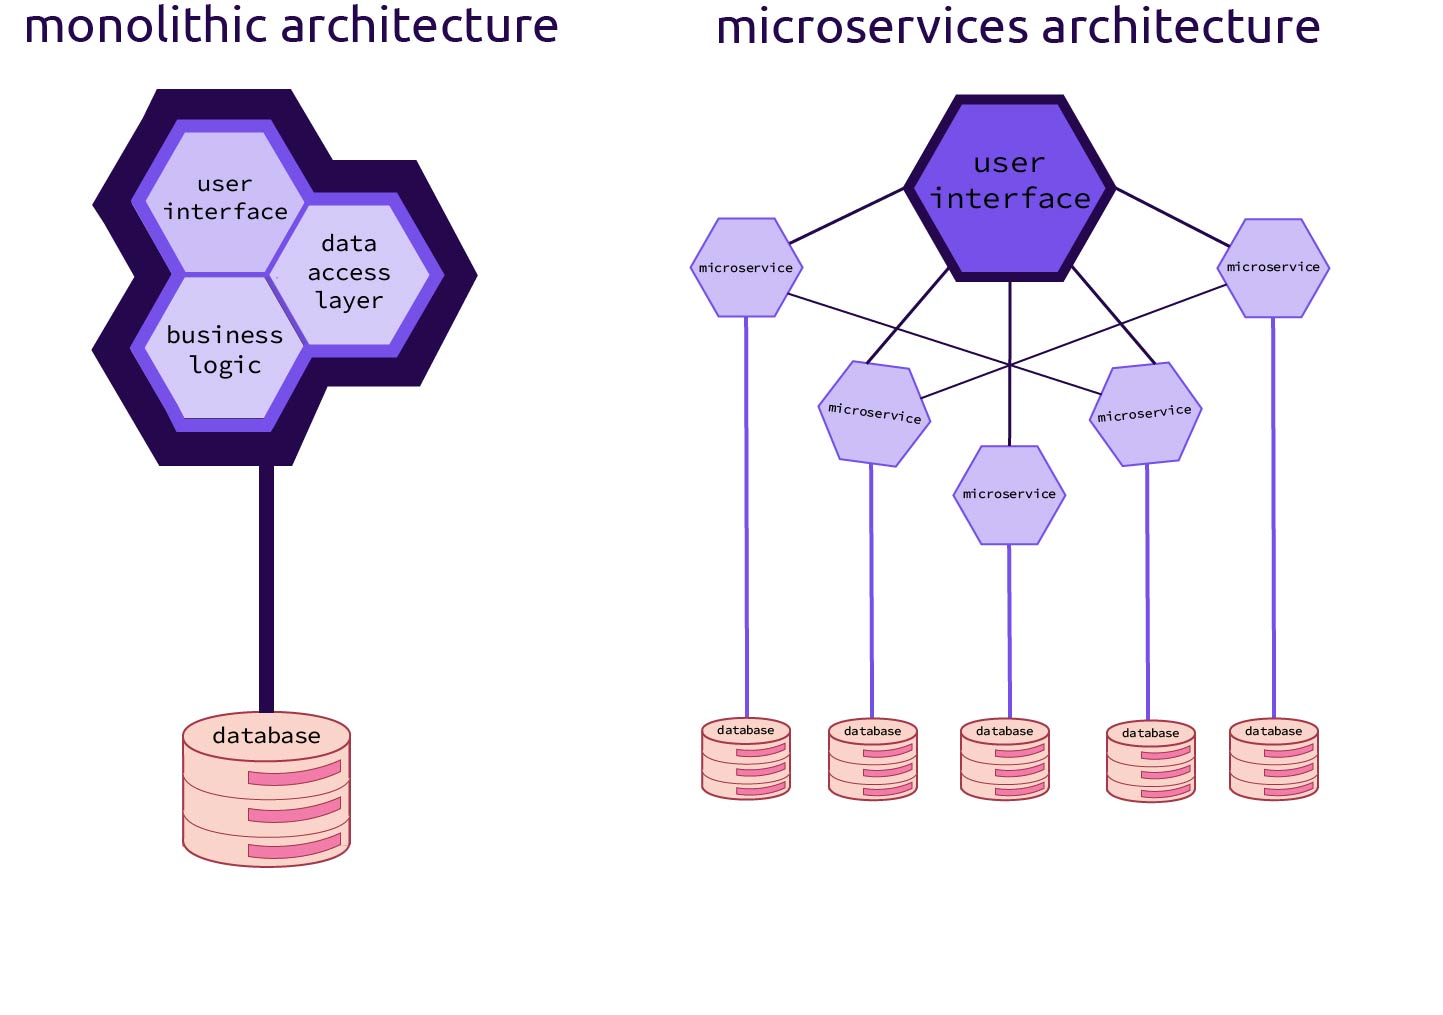
\includegraphics[width=1\textwidth]{Images/monoliths-vs-microservices-whats-the-difference_2.png}
  \caption{MicroServices vs Monolithic}
  \label{fig:microservicesVmonolithic}
\end{figure}

\section{Batch Job Execution}

Batch processing refers to the execution of non-interactive, background jobs that process data in large volumes~\cite{batch-processing}. 
Unlike real-time systems, batch jobs are scheduled and executed at specified times or on demand, often in isolated environments.

Kubernetes natively supports batch job execution through the \texttt{Job} and \texttt{CronJob} resources. In the designed system, 
batch jobs are launched on behalf of users to run data analysis scripts using containerized tools like DuckDB or Pandas, with each 
job being tracked and managed independently.

\section{MinIO}

\begin{figure}[h!]
  \centering
  
\includegraphics[width=0.5\textwidth]{Images/minIO.png}
  \caption{MinIO}
  \label{fig:minio}
\end{figure}

MinIO is a high-performance, Kubernetes-native object storage system compatible with the Amazon S3 API~\cite{minio-docs}. 
It is often used in cloud-native applications to store unstructured data such as logs, images, or datasets.

In the system, MinIO acts as the backend storage for user-uploaded files and job outputs. Its compatibility with S3 allows for flexible 
integration with analytics tools and easy management of large datasets without a traditional POSIX filesystem. 

Additionally, the imaged application tools used in the system are set with I/O on MinIO.
\section{DuckDB}

DuckDB is an in-process SQL OLAP (Online Analytical Processing) database management system optimized for analytical queries on 
columnar data~\cite{duckdb-paper}. Unlike traditional database servers, DuckDB runs directly within the host process and is designed for interactive 
analytics on local files such as CSV and Parquet. Its columnar storage model and vectorized query execution engine make it particularly 
suitable for analytical workloads involving large datasets.

DuckDB draws conceptual inspiration from systems like PostgreSQL and MonetDB, but emphasizes lightweight deployment and embeddability. 
It supports complex SQL queries, window functions, joins, and aggregations with high performance, while avoiding the operational 
complexity of client-server architectures.

\subsection*{Why DuckDB?}

\begin{figure}[h!]
  \centering
  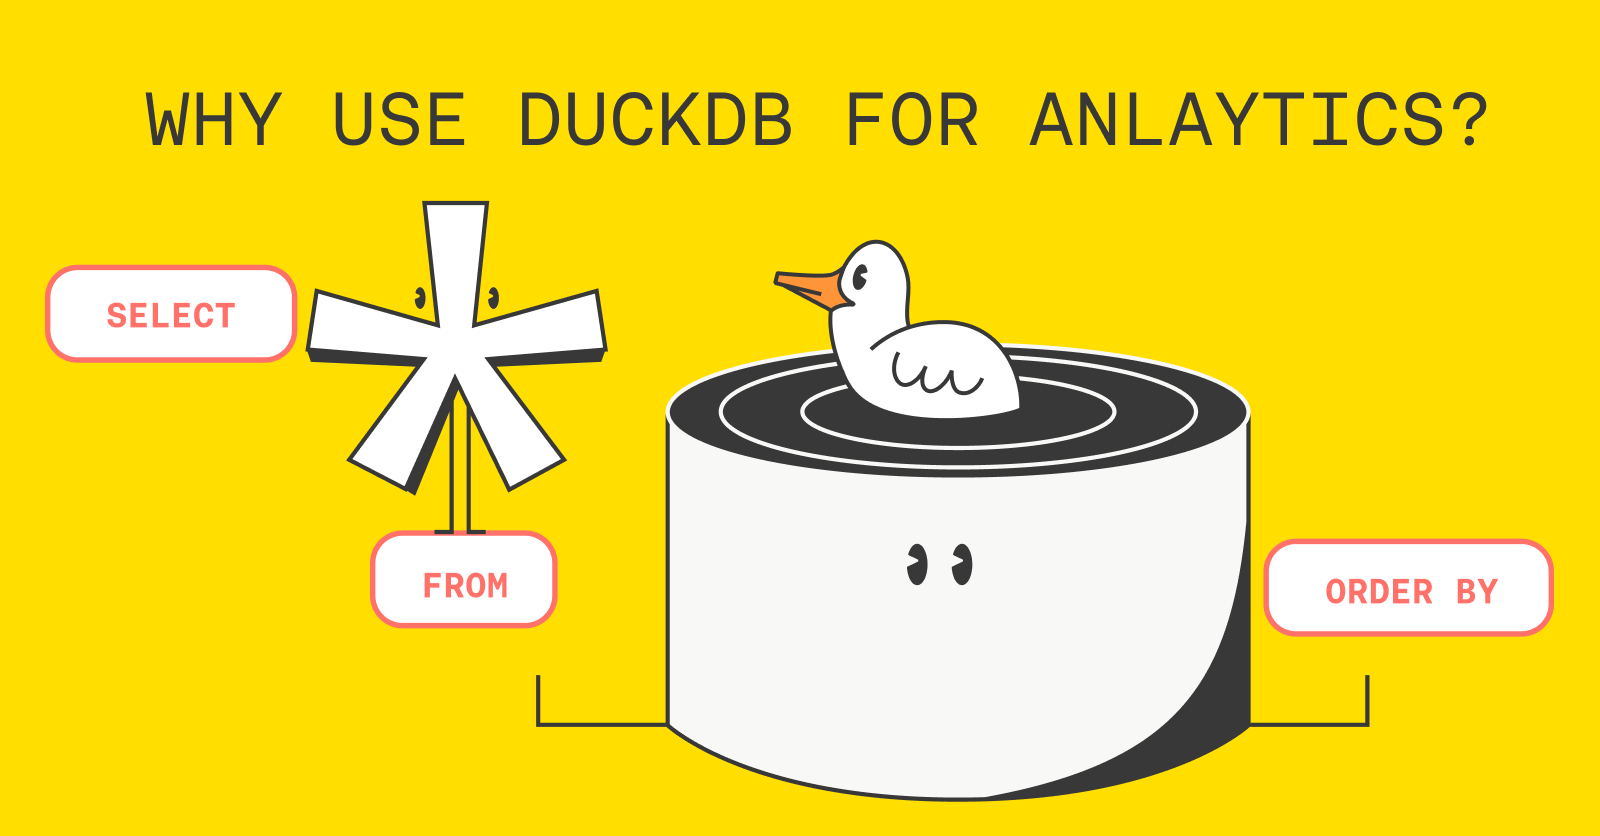
\includegraphics[width=1\textwidth]{Images/duckdb_for_analytics_1_c16a0acfc3.png}
  \caption{Why DuckDB}
  \label{fig:duckdb}
\end{figure}

DuckDB was chosen for this system due to several compelling advantages:

\begin{itemize}
    \item \textbf{Embeddability:} DuckDB can be run inside a container with no setup or external dependencies, making it ideal for 
    sandboxed job execution in Kubernetes.
    
    \item \textbf{Zero Configuration:} Users can query structured files (e.g., CSV, Parquet) without needing to first load data 
    into database tables, simplifying the user workflow.
    
    \item \textbf{Columnar Execution:} Optimized for analytical queries, DuckDB's columnar execution model enables efficient 
    processing of large datasets, particularly in filtering and aggregation operations.
    
    \item \textbf{File-Native Access:} Direct support for querying local data files stored on persistent volumes or object 
    storage simplifies integration with the storage layer (MinIO).
    
    \item \textbf{Lightweight and Fast:} Compared to heavier analytical engines, DuckDB has a small footprint and fast startup time, 
    which makes it suitable for short-lived Kubernetes jobs.
\end{itemize}

In this system, DuckDB is one of the containerized tools available for users to execute SQL-based data analysis jobs on uploaded datasets. 
Its integration enables users to perform complex transformations and analytics directly on their data without managing database 
infrastructure.

\section{SQLite}

\begin{figure}[h!]
  \centering
  
\includegraphics[width=0.5\textwidth]{Images/sqlite-chatgpt-img.png}
  \caption{SQLite}
  \label{fig:sqlite}
\end{figure}

SQLite is a lightweight, serverless, self-contained SQL database engine~\cite{sqlite-docs}. Unlike traditional client-server databases, 
SQLite operates directly on a single disk file and does not require a separate database server process. Its simplicity, low resource 
overhead, and zero-configuration nature make it an ideal choice for embedded applications and local data persistence.

In this system, SQLite is used as the backend storage mechanism for several services, including authentication (Minioth), 
filesystem metadata (Fslite), and job tracking (Uspace). Each service maintains its own isolated SQLite instance, ensuring 
modularity and local data consistency. The relational model of SQLite provides a robust framework for enforcing constraints, 
indexing, and transactional integrity, all while maintaining high performance for low- to moderate-volume workloads.

Due to its embeddable nature, SQLite enables rapid development and deployment of microservices without the overhead of managing 
a centralized database server. This aligns well with the platform’s goals of simplicity, portability, and lightweight infrastructure.


\section{WebSockets}
\begin{figure}[h!]
  \centering
  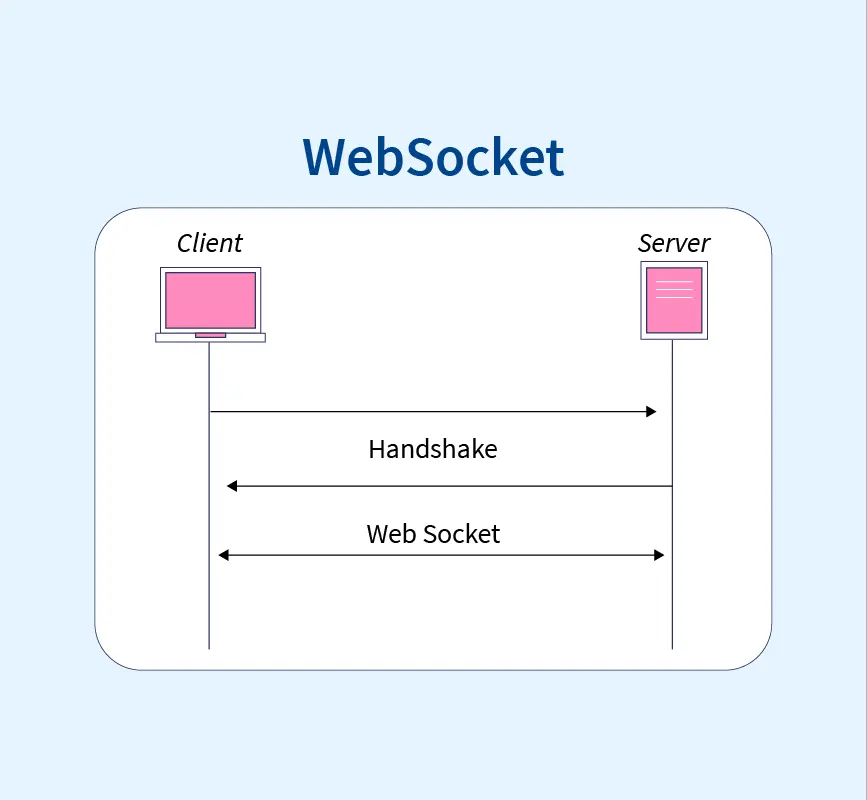
\includegraphics[width=0.8\textwidth]{Images/websockets-1.png}
  \caption{WebSockets}
  \label{fig:websockets}
\end{figure}

WebSockets provide a full-duplex communication channel over a single TCP connection, allowing real-time interaction between 
clients and servers~\cite{ietf-websocket}. Unlike traditional HTTP, WebSockets maintain a persistent connection, enabling low-latency communication.

The system utilizes WebSockets to allow users to interact with their environment in real time, including job monitoring and 
event-driven communication with backend services.
\section{Containers}

\begin{figure}[h!]
  \centering
  
\includegraphics[width=0.5\textwidth]{Images/what-is-docker.png}
  \caption{Docker Containers}
  \label{fig:docker-containers}
\end{figure}

Containers are lightweight, portable units that package software with its dependencies and run isolated from the host 
system~\cite{docker-docs}. Technologies like Docker and container runtimes such as containerd have made containers a 
standard deployment model in modern systems.

In this system, each analytical job is executed within its own container, ensuring environment reproducibility and isolation 
between users. This also facilitates the inclusion of tools like Bash, Octave, and Python in a controlled, sandboxed manner.

The Microservices theirselves will be deployed as individual containers in collaboration with K8S.
\section{Multi-User System Design}

A multi-user system is one that supports concurrent access by multiple independent users, often with varying levels of access, 
permissions, and isolation. In such systems, key design considerations include authentication, authorization, resource sharing, 
and conflict avoidance~\cite{tanenbaum-os}.

The platform presented in this thesis implements a multi-user architecture where each user is assigned a secure, isolated environment. 
Users may upload datasets, execute jobs, and share resources depending on their group memberships and permissions. This design is 
inspired by UNIX-like models, incorporating user/group-based access control to enforce data protection and operational boundaries 
within a shared infrastructure.

\newpage
\section{Authentication Model}

Authentication is the process of verifying the identity of users before granting access to system resources~\cite{ferraiolo-auth}. 
In multi-user systems, secure and reliable authentication is foundational to ensuring that only authorized users can interact with 
sensitive data or operations.

The system utilizes a custom-built authentication service called \texttt{Minioth}, which follows a token-based authentication scheme 
using JSON Web Tokens (JWT). Upon successful login, users receive short-lived signed tokens that are used to authenticate future requests. 
This stateless approach enables efficient, scalable identity verification across distributed microservices, while also supporting user and 
group management for access control.

\newpage
\section{Cloud-Native Storage}

\begin{figure}[h!]
  \centering
  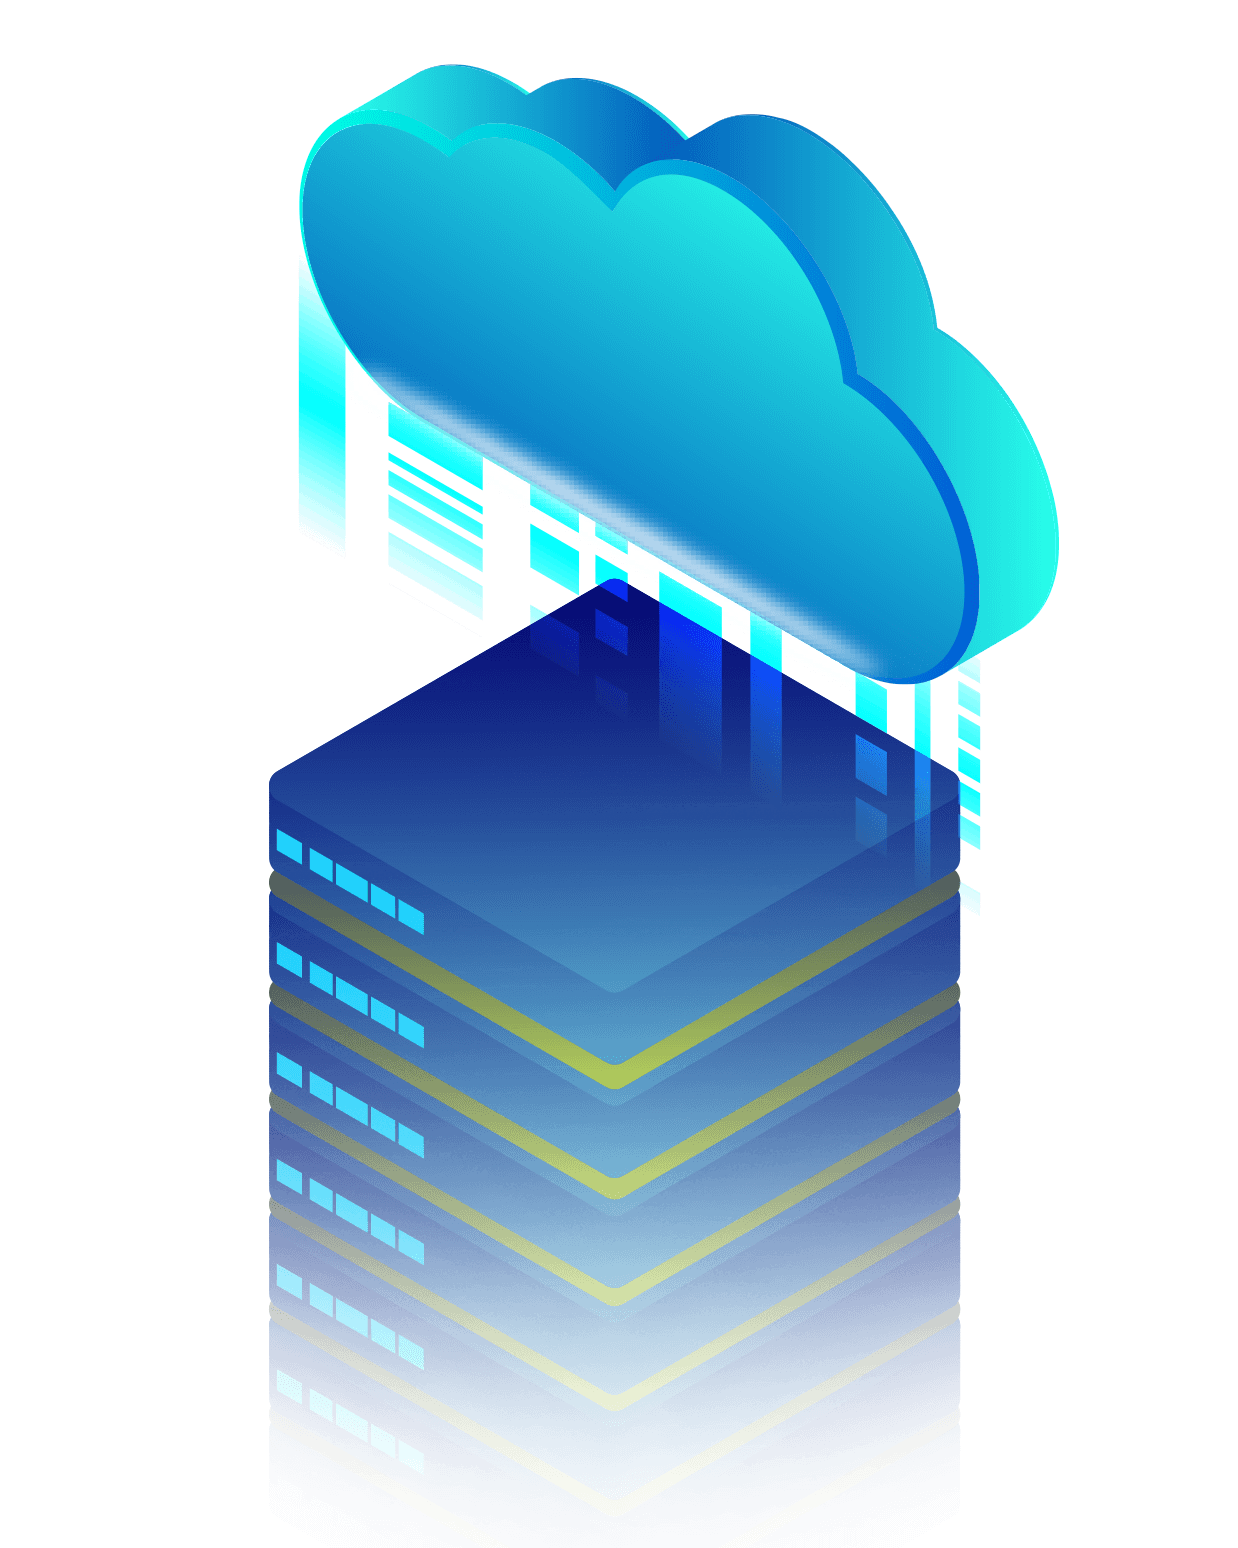
\includegraphics[width=0.4\textwidth]{Images/img-hybrid-cloud-engineer.png}
  \caption{CNS}
  \label{fig:cns}
\end{figure}

Cloud-native storage refers to storage systems designed to operate within cloud environments, typically containerized and orchestrated 
via platforms like Kubernetes~\cite{cncf-storage}. Unlike traditional block or file-based storage, cloud-native storage solutions are 
optimized for dynamic workloads, scalability, and high availability.

In this system, MinIO—a cloud-native object storage service compatible with Amazon S3—is used to store user data and job outputs. 
Object storage offers flexibility in managing large, unstructured datasets, and integrates seamlessly with Kubernetes via 
Persistent Volume Claims (PVCs). Cloud-native storage allows the system to dynamically provision isolated storage volumes for each 
user or job, supporting scalable and fault-tolerant operations.


\chapter{Related Work}
\label{Chapter-Related-Work}

% Todo: Edit to your liking
\section{Related work A}
\section{Related work B}

\section{The FPGA Perspective}
\section{Thesis Approach}

\chapter{System Design and Architecture}
\label{Chapter-SystemDesign-Architecture}



\section{Overview diagram}
\begin{figure}[h!]
  \centering
  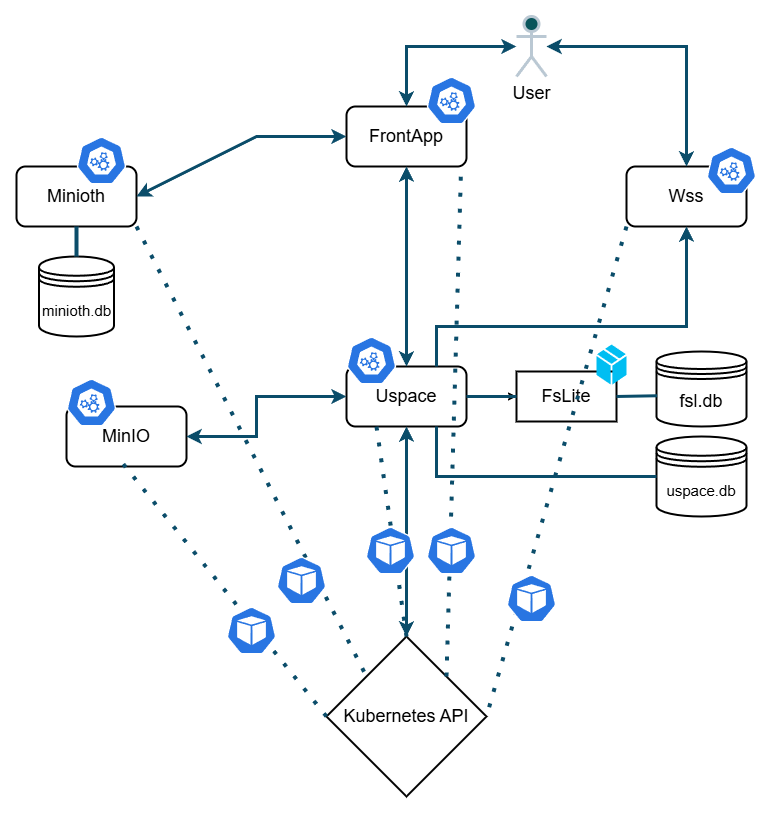
\includegraphics[width=1\textwidth]{Images/kuspace-overview.png}
  \caption{Kuspace System Overview}
  \label{fig:kuspace-overview}
\end{figure}


\begin{figure}[h!]
  \centering
  
\includegraphics[width=0.5\textwidth]{Images/kuspace-logo.png}
  \caption{Kuspace logo}
  \label{fig:kuspace-overview}
\end{figure}


\section{Minioth: Authentication Service}

Minioth~\cite{minioth} is a custom authentication and authorization microservice responsible for managing user identities and enforcing access control
within the system. It implements a secure token-based authentication model using JSON Web Tokens (JWT)~\cite{jwt-spec}, allowing users to authenticate
once and interact with other services securely.

\begin{figure}[h]
  \centering
  
\includegraphics[width=0.3\textwidth]{Images/minioth_logo_chatgpt_draft1.png}
  \caption{Minioth logo}
  \label{fig:miniothlogo}
\end{figure}

Minioth supports essential user and group management operations such as registration, login, group assignment, and permission checking.
It exposes a RESTful API~\cite{fielding-rest} that other services use to validate user tokens and retrieve identity-related metadata (e.g., UID, GID). 
This decouples authentication logic from the rest of the system, promoting modularity and reusability.

All user interactions begin with Minioth, and its integration is critical to enabling multi-user isolation, secure job execution, and 
controlled access to shared data resources.

Minioth aspires to become a fully capable identity provider!

\subsection{Authorization Details}

Minioth implements a simplified Role-Based Access Control (RBAC) model centered around user groups. Each user is assigned a unique primary group upon creation, which serves as the basis for resource ownership and sharing semantics. Group membership information is embedded in the issued JWTs, enabling downstream services to perform access checks without additional lookups.

At present, the system distinguishes between regular users and administrators. Membership in the \texttt{admin} group grants elevated privileges, including access to user and group management endpoints, system introspection, and key rotation. All other users are constrained to operations permitted within their assigned roles and groups.

\subsection{Authentication Details}

The Minioth authentication service implements secure, configurable user login and token issuance. Upon a successful login request via the \texttt{POST /login} endpoint, the system issues a JSON Web Token (JWT) containing the authenticated user's identity claims.

\paragraph{Token Signing Algorithm}
Clients can specify the desired signing algorithm by including the optional HTTP header:

\begin{quote}
\texttt{X-Auth-Signing-Alg: HS256} \quad or \quad \texttt{RS256}~\cite{jose-algorithms}
\end{quote}

\begin{itemize}
  \item \textbf{HS256} — HMAC using SHA-256~\cite{sha256-rfc6234}, with a system-defined shared secret.
  \item \textbf{RS256} — RSA signature using SHA-256, with a system-configured private/public key pair. 
  The public key is exposed via the JWKS endpoint (\texttt{/.well-known/jwks.json}).
\end{itemize}

If the header is omitted, the system uses the default signing algorithm defined in the configuration file. 
This design supports interoperability with external identity providers and ensures future extensibility toward OpenID Connect.

\paragraph{Password Hashing}
User passwords are never stored in plain text. Instead, all passwords are hashed using the \textbf{bcrypt}~\cite{bcrypt} 
algorithm prior to storage. The hashing cost (also referred to as the computational work factor) is system-defined and configurable. 
It controls the computational difficulty of the hashing process, allowing the system to be tuned for performance versus security:

\begin{algorithm}
\caption{Password Hashing using \texttt{bcrypt}}\label{alg:bcrypt}
\begin{algorithmic}[1]
\Procedure{HashPassword}{$password, cost$}
    \State $salt \gets \text{GenerateSalt}(cost)$
    \State $hash \gets \text{Bcrypt}(password, salt)$
    \State \Return $hash$
\EndProcedure
\end{algorithmic}
\end{algorithm}


A higher cost increases the time required to compute the hash, improving resistance to brute-force attacks at the expense of login speed.

\subsection{Pluggable Authentication Handlers}

Minioth is designed with extensibility in mind, offering a flexible backend architecture based on pluggable \textit{handlers}. A handler is a concrete implementation of a unified interface responsible for managing users, groups, and authentication state.

This architecture decouples the authentication logic from the underlying storage mechanism, enabling multiple interchangeable backends with minimal effort. All handlers implement the following interface:

\begin{algorithm}[H]
\caption{Abstract Handler Interface (pseudocode)}
\begin{algorithmic}
\Function{Init}{}
\EndFunction

\Function{UserAdd}{User}
  \State Returns: (UID, primaryGroup, Error)
\EndFunction

\Function{UserDel}{UID}
\EndFunction

\Function{UserMod}{User}
\EndFunction

\Function{UserPatch}{UID, Fields}
\EndFunction

\Function{GroupAdd}{Group}
  \State Returns: (GID, Error)
\EndFunction

\Function{GroupDel}{GID}
\EndFunction

\Function{GroupMod}{Group}
\EndFunction

\Function{GroupPatch}{GID, Fields}
\EndFunction

\Function{Authenticate}{Username, Password}
  \State Returns: User or Error
\EndFunction

\Function{Select}{ID}
  \State Returns: Any
\EndFunction

\Function{Purge}{}
\EndFunction

\Function{Close}{}
\EndFunction
\end{algorithmic}
\end{algorithm}



\paragraph{Available Handlers:}
\begin{itemize}
    \item \textbf{Database Handler:}  
    A fully featured implementation that uses a relational database backend (such as SQLite or DuckDB). This handler persists user, group, and credential data in structured tables, enabling query flexibility, indexing, and transactional safety.

    \item \textbf{Plain Handler:}  
    A minimalist implementation that stores user-related data in three flat files, following a UNIX-like structure:
    \begin{itemize}
        \item \texttt{mpasswd} — stores basic user account data (username, UID, GID)
        \item \texttt{mgroup} — stores group records (name, GID, members)
        \item \texttt{mshadow} — stores password hashes
    \end{itemize}
    This mode is particularly useful for lightweight deployments, testing, or portability.
\end{itemize}

Each handler supports core operations such as user/group creation, deletion, modification, and password-based authentication. 
By implementing the same interface, they are interchangeable at runtime, allowing the system to be easily configured for 
different deployment targets or performance/security trade-offs. 

New handlers suitable for other databases can be implemented.

\begin{figure}[h!]
  \centering
  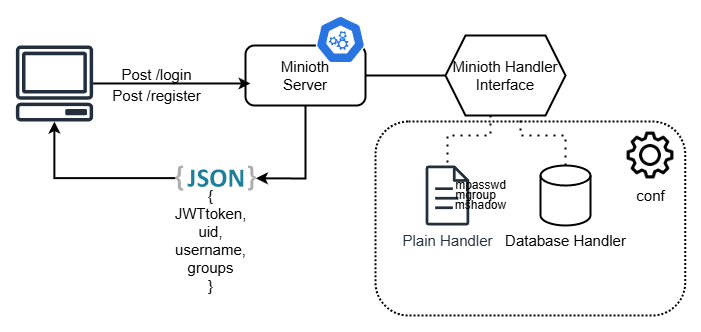
\includegraphics[width=1\textwidth]{Images/minioth-blockdiagram.png}
  \caption{Minioth Block Diagram}
  \label{fig:minioth-blockdiagram}
\end{figure}

\subsection{Minioth Public API Endpoints}

\begin{table}[H]
\centering
\resizebox{\textwidth}{!}{%
\begin{tabular}{|l|l|p{7cm}|c|}
\hline
\textbf{Method} & \textbf{Path} & \textbf{Description} & \textbf{Auth} \\
\hline
\hline
POST  & \texttt{/v1/register}            & Register a new user.                           & No  \\
POST  & \texttt{/v1/login}               & Authenticate and receive JWT token.            & No  \\
POST  & \texttt{/v1/passwd}              & Change password for the authenticated user.    & Yes (user/admin) \\
GET   & \texttt{/v1/user/me}             & Get information about the token's user.        & Token \\
GET   & \texttt{/v1/user/token}          & View current token details.                    & No \\
POST  & \texttt{/v1/user/refresh-token}  & Request a new access token using a refresh token. & No \\
GET   & \texttt{/v1/swagger/*any}        & Swagger UI for live API documentation.         & No \\
\hline
\hline
\end{tabular}%
}
\caption{Minioth public/user API endpoints}
\label{tab:minioth-public-endpoints}
\end{table}

\subsection{Minioth Admin API Endpoints}

\begin{table}[H]
\centering
\resizebox{\textwidth}{!}{%
\begin{tabular}{|l|l|p{7cm}|c|}
\hline
\textbf{Method} & \textbf{Path} & \textbf{Description} \\
\hline
\hline
GET    & \texttt{/v1/admin/audit/logs}      & Retrieve system audit logs. \\
POST   & \texttt{/v1/admin/hasher}          & Generate bcrypt hashes from plaintext passwords. \\
POST   & \texttt{/v1/admin/verify-password} & Compare a password against a stored hash. \\
GET    & \texttt{/v1/admin/users}           & List all registered users. \\
GET    & \texttt{/v1/admin/groups}          & List all groups and their members. \\
POST   & \texttt{/v1/admin/useradd}         & Add a new user to the system. \\
DELETE & \texttt{/v1/admin/userdel}         & Delete a user by UID or username. \\
PATCH  & \texttt{/v1/admin/userpatch}       & Update selected fields of a user. \\
PUT    & \texttt{/v1/admin/usermod}         & Fully replace a user record. \\
POST   & \texttt{/v1/admin/groupadd}        & Create a new group. \\
PATCH  & \texttt{/v1/admin/grouppatch}      & Update specific fields of a group. \\
PUT    & \texttt{/v1/admin/groupmod}        & Fully update a group definition. \\
DELETE & \texttt{/v1/admin/groupdel}        & Remove a group from the system. \\
POST   & \texttt{/v1/admin/rotate}          & Rotate the JWT signing key in use. \\
GET    & \texttt{/v1/admin/system-conf}     & View current server configuration. \\
\hline
\hline
\end{tabular}%
}
\caption{Minioth public/admin API endpoints}
\label{tab:minioth-public-endpoints}
\end{table}

Essentially admin features include full user/group lifecycle management and 
audit logging, key rotation and token inspection mechanisms.

An Authorization header is required with the JWT token as a Bearer.

\subsection{Integration}

Minioth is integrated into the overall system architecture as a Kubernetes StatefulSet, with user and group data persisted on a dedicated Persistent Volume Claim (PVC). It serves as the central authentication authority by issuing JWT tokens consumed by other services, primarily the Frontend application, to authorize user actions.

To ensure secure inter-service communication, all microservices, including Minioth, share a common \texttt{ServiceSecret} key. This key enables mutual trust and token verification across services. Additionally, the JWT signing key is generated at deployment time via a configurable secret generator and securely injected into the Minioth service configuration.


\newpage



\section{Uspace: Central Orchestration and Job Management Service}
\label{sec:uspace}

The \textbf{Uspace} service constitutes the core of the system’s architecture, 
acting as the central orchestration unit that coordinates job scheduling, 
storage access, and user-level interaction with analytical resources. 
It is built with extensibility and modularity in mind, offering a consistent 
interface between users, applications, and the underlying infrastructure.

\subsection{Responsibilities and Purpose}

Uspace maintains the persistent state of the system through:
\begin{itemize}
    \item A resource and volume metadata store powered by the \texttt{FsLite} module.
    \item A local database (SQLite or DuckDB) for tracking user-submitted jobs and available applications.
    \item A job scheduling and dispatch pipeline which integrates with the Kubernetes API.
\end{itemize}

Uspace exposes a RESTful API to authenticated users and administrators, supporting operations such as uploading datasets, browsing resources, and launching computational jobs.

\newpage

\begin{table}[H]
\centering
\resizebox{\textwidth}{!}{%
\begin{tabular}{|l|l|p{9cm}|c|}
\hline
\textbf{Method} & \textbf{Path} & \textbf{Description} & \textbf{Requires \texttt{Access-Target}} \\
\hline
GET & \texttt{/healthz} & Health check endpoint. & No \\
GET/POST & \texttt{/api/v1/job} & Submit or list jobs. & No \\
GET/POST & \texttt{/api/v1/app} & List available tools (applications). & No \\
GET & \texttt{/api/v1/resources} & List resources (“ls” equivalent). & Yes \\
POST & \texttt{/api/v1/resource/upload} & Upload a new resource file. & Yes \\
GET & \texttt{/api/v1/resource/preview} & Preview a resource. & Yes (Read) \\
GET & \texttt{/api/v1/resource/download} & Download a resource. & Yes (Read) \\
DELETE & \texttt{/api/v1/resource/rm} & Delete a resource. & Yes (Write) \\
POST & \texttt{/api/v1/resource/cp} & Copy a resource. & Yes (Read) \\
PATCH & \texttt{/api/v1/resource/mv} & Move/rename a resource. & Yes (Write) \\
PATCH & \texttt{/api/v1/resource/permissions} & Change resource permissions. & Yes (Owner) \\
PATCH & \texttt{/api/v1/resource/ownership} & Change resource ownership. & Yes (Owner) \\
PATCH & \texttt{/api/v1/resource/group} & Change associated group. & Yes (Owner) \\
\hline
\end{tabular}
}
\caption{Uspace User API Endpoints}
\label{tab:uspace-user-endpoints}
\end{table}


\begin{table}[H]
\centering
\resizebox{\textwidth}{!}{%
\begin{tabular}{|l|l|p{9cm}|}
\hline
\textbf{Method} & \textbf{Path} & \textbf{Description} \\
\hline
GET/POST/PUT/DELETE/PATCH & \texttt{/api/v1/admin/volumes} & Full volume management API. \\
DELETE/PUT & \texttt{/api/v1/admin/job} & Administrative job control (e.g., delete jobs). \\
GET/POST/PATCH/DELETE & \texttt{/api/v1/admin/user/volume} & Manage user-volume mappings. \\
GET/POST/PUT/DELETE & \texttt{/api/v1/admin/app} & Manage available applications/tools. \\
GET & \texttt{/api/v1/admin/system-conf} & View current system configuration. \\
GET & \texttt{/api/v1/admin/system-metrics} & System metrics via Kubernetes API. \\
\hline
\end{tabular}
}
\caption{Uspace Admin API Endpoints}
\label{tab:uspace-admin-endpoints}
\end{table}

\subsection{Middleware and Access Control}

The Uspace API applies layered middleware to enforce authentication, authorization, and request context binding.

In particular, API endpoints require a custom HTTP header named \texttt{Access-Target}, which encodes the target resource and the user identity. The header follows this format:

\begin{verbatim}
Access-Target: <volume_id>:<volume_name>:<resource_path> 
<user_id>:[group_id1,group_id2,...]
\end{verbatim}

The middleware parses this value to construct an \texttt{AccessClaim} object, which is then used to evaluate permissions through FsLite. This mechanism abstracts identity and access metadata away from individual endpoint logic and enforces consistency across resource operations.

Only authorized users (based on ownership or group permissions) can perform operations such as previewing, downloading, modifying, or deleting resources.

Furthermore, all API groups apply the \texttt{serviceAuth} middleware for validating a ServiceSecret common in the Service and verifying the caller is only a service in the system.

\subsection{Core Structure}

At the heart of the system lies the \texttt{UService} object, which encapsulates the configuration, runtime engine, and modular components responsible for storage, job handling, and resource management. Its composition is summarized as follows:

\begin{itemize}
    \item \textbf{Configuration (\texttt{config})}: Encapsulates all environment-based settings loaded during service initialization. This allows flexible configuration for both development and production deployments.
    
    \item \textbf{Web Engine (\texttt{Engine})}: A Gin-based HTTP server that handles incoming API requests and routes them to appropriate handlers. It also includes middleware for authentication and authorization.
    
    \item \textbf{Storage Backend (\texttt{storage})}: Implements the \texttt{StorageSystem} interface. In this system, it uses a MinIO-based implementation for interacting with S3-compatible object storage. The interface, however, allows for future pluggability (e.g., plain file volumes).
    
    \item \textbf{Job Database Handler (\texttt{jdbh})}: Provides access to the local DuckDB or SQLite database used to track job submissions, statuses, and registered analytical applications.
    
    \item \textbf{Filesystem Metadata Layer (\texttt{fsl})}: An instance of FsLite, used as an internal metadata engine for enforcing user-based access controls and tracking virtual filesystem hierarchies over the object store.
    
    \item \textbf{Job Dispatcher (\texttt{jdp})}: Orchestrates the submission and lifecycle of analytical jobs. It abstracts the underlying execution backend (e.g., Kubernetes or Docker), enabling future extensibility via the \texttt{JobDispatcher} interface.
\end{itemize}


\newpage

\subsection{Storage Provider Abstraction}

The \texttt{StorageSystem} interface defines the contract for interacting with storage backends. Below is a description of its main methods:

\begin{algorithm}[H]
\caption{Abstract \texttt{StorageSystem} Interface (pseudocode)}
\begin{algorithmic}[1]

\Function{DefaultVolume}{local: Bool}
  \State \Return default volume identifier as String
\EndFunction

\Function{CreateVolume}{volume: Any}
  \State \Return Error if creation fails
\EndFunction

\Function{SelectVolumes}{criteria: Map[String, Any]}
  \State \Return matching volumes or Error
\EndFunction

\Function{SelectObjects}{criteria: Map[String, Any]}
  \State \Return matching objects or Error
\EndFunction

\Function{Insert}{object: Any}
  \State \Return CancelFunc, Error
\EndFunction

\Function{Download}{object: Any}
  \State \Return CancelFunc, Error
\EndFunction

\Function{Stat}{object: Any}
  \State \Return metadata or Error
\EndFunction

\Function{Remove}{object: Any}
  \State \Return Error
\EndFunction

\Function{RemoveVolume}{volume: Any}
  \State \Return Error
\EndFunction

\Function{Update}{metadata: Map[String, String]}
  \State \Return Error
\EndFunction

\Function{Copy}{source: Any, dest: Any}
  \State \Return Error
\EndFunction

\Function{Share}{method: String, object: Any}
  \State \Return SharingDescriptor or Error
\EndFunction

\end{algorithmic}
\end{algorithm}


\newpage
\subsection{Storage Control}
Uspace as mentioned handles storage in two layers. 
\begin{itemize}

\item  The metadata layer that includes access control is consisted of \texttt{FsLite} module which also 
enforces authorization on the resources.
\item The \texttt{StorageSystem} for physical storage, MinIO, and its API is accessed by a custom Go MinIO client.
\end{itemize}


\begin{figure}[h]
  \centering
  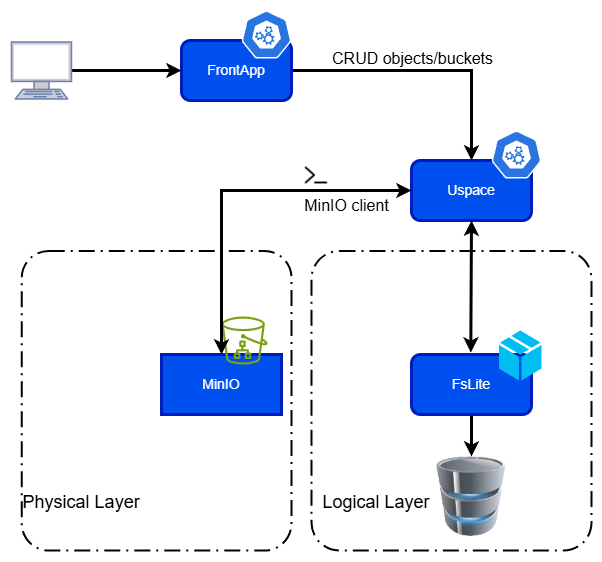
\includegraphics[width=1\textwidth]{Images/UspaceBlockDiagram.drawio.png}
  \caption{Uspace Storage Overview}
  \label{fig:uspace-storage-overview}
\end{figure}

\subsection{Job Dispatcher and Executor}

Uspace includes a pluggable job dispatching mechanism defined by the \texttt{JobDispatcher} interface,
as well as a job execution mechanism defined by the \texttt{JobExecutor} interface:

\begin{algorithm}[H]
\caption{Abstract \texttt{JobDispatcher} Interface (pseudocode)}
\label{alg:job-dispatcher}
\begin{algorithmic}[1]

\Function{Start}{}
  \State Initialize and begin dispatching system
\EndFunction

\Function{PublishJob}{job: Job}
  \State Submit a single job for dispatch
  \State \Return Error on failure
\EndFunction

\Function{PublishJobs}{jobs: List[Job]}
  \State Submit a batch of jobs
  \State \Return Error on failure
\EndFunction

\Function{RemoveJob}{jobID: Integer}
  \State Cancel or remove job with given ID
  \State \Return Error on failure
\EndFunction

\Function{RemoveJobs}{jobIDs: List[Integer]}
  \State Remove multiple jobs
  \State \Return Error on failure
\EndFunction

\Function{Subscribe}{job: Job}
  \State Register job for event handling or feedback
  \State \Return Error on failure
\EndFunction

\end{algorithmic}
\end{algorithm}

\begin{algorithm}[H]
\caption{Abstract \texttt{JobExecutor} Interface (pseudocode)}
\begin{algorithmic}
\Function{ExecuteJob}{job}
  \State Returns: Error
\EndFunction

\Function{CancelJob}{job}
  \State Returns: Error
\EndFunction

\end{algorithmic}
\end{algorithm}



The default implementation is a \texttt{JobManager}, which maintains queues and internal execution tracking. It uses a \texttt{JobExecutor} to actually launch jobs using one of two backends:
\begin{itemize}
    \item \textbf{DockerExecutor}: Launches jobs in local Docker containers for testing.
    \item \textbf{KubernetesExecutor}: Launches Kubernetes Jobs via the API for production workloads.
\end{itemize}

This separation of concerns enables the system to evolve with future support for alternative execution engines such as serverless functions or distributed clusters.

\textbf{Job Specification}: Each submitted job is described by a structured payload that defines its resource requirements, execution logic, and metadata.

The job object includes:

\begin{itemize}
    \item \textbf{Identifiers:} \texttt{JID} (Job ID), \texttt{UID} (User ID).
    \item \textbf{Resource Requirements:} CPU, memory, and ephemeral storage requests/limits.
    \item \textbf{Execution Parameters:} \texttt{Parallelism}, \texttt{Timeout}, \texttt{Priority}.
    \item \textbf{Paths:} \texttt{Input} and \texttt{Output} resource references.
    \item \textbf{Logic:} A predefined \texttt{Logic} (e.g., ``duckdb'') and a \texttt{LogicBody} representing the code or command to be executed.
    \item \textbf{Environment:} An optional key-value map of environment variables.
    \item \textbf{Status Tracking:} Includes current \texttt{Status}, \texttt{CreatedAt}, \texttt{CompletedAt}, and a boolean \texttt{Completed} flag.
\end{itemize}

Jobs are submitted through the Uspace API, validated, and dispatched for execution by the internal job manager. The structure supports extensibility for both containerized tools and script execution across different runtimes.

\subsection{Job Execution Pipeline}
\textbf{Job Execution} in Uspace follows as:
\begin{enumerate}
  \item The user submits a job definition via \texttt{/job}.
  \item The \texttt{JobDispatcher} validates and prepares the job.
  \item The \texttt{JobManager} handles scheduling and preparation for Kubernetes.
  \item The \texttt{JobExecutor} decides upon the existing imaged applications, and sets up the appropriate variables and connections for I/O to the Storage System
  \item The \texttt{JobExecutor} then launches the containerized workload on the Engine Execution Model (e.g Kubernetes API Jobs).
  \item Runtime results are streamed to WSS and the output is saved on the Storage Provider (MinIO) of the path specified.
\end{enumerate}

All jobs are tracked in the local job database with associated metadata, status, timestamps, and references to input/output files.

\subsection{Job Scheduling}

The \texttt{Uspace} service includes an embedded job scheduling mechanism implemented by the \texttt{JobManager} component. It operates on a producer-consumer model, where jobs submitted by authenticated users are pushed into a bounded queue (\texttt{jobQueue}). The size of this queue is configurable via \texttt{UspaceJobQueueSize}, defaulting to 100 entries.

Job execution is handled concurrently by a worker pool, constrained by a configurable parameter (\texttt{UspaceJobMaxWorkers}). Each job is processed in a dedicated goroutine, with the pool enforced via a buffered channel (\texttt{workerPool}) to prevent system overload.

When a job is dequeued, it is dispatched to the selected \texttt{JobExecutor}—either Docker-based or Kubernetes-based—determined during service initialization. This separation allows for modular testing and cloud-native deployment.

If the job queue is full, submissions are rejected, providing backpressure to upstream services or users. This model ensures that the system maintains a predictable load and resource profile.

\newpage

\begin{figure}[h]
  \centering
  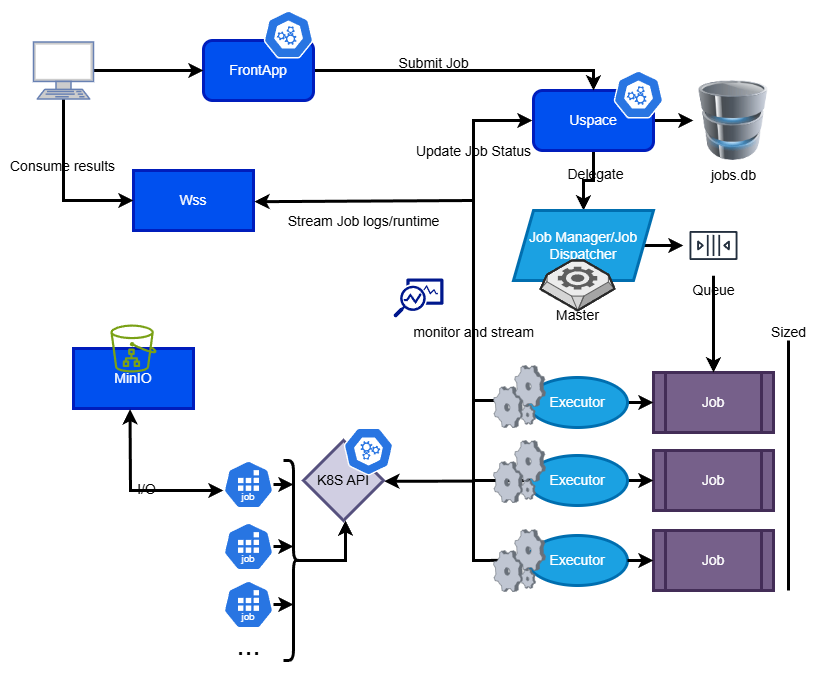
\includegraphics[width=1\textwidth]{Images/job-lifecycle.png}
  \caption{Job Lifecycle}
  \label{fig:job-lifecycle}
\end{figure}


\subsection{Available Applications}

The Uspace system supports a set of containerized applications that can be executed as jobs. These applications are defined as Docker images with a uniform execution contract. Each application:

\begin{itemize}
    \item Receives the input and output paths via environment variables.
    \item Uses preconfigured MinIO credentials to fetch and store data.
    \item Executes its logic using the input file(s) and writes the results to the specified output location in MinIO.
\end{itemize}

The current applications integrated into the system are shown in Table~\ref{tab:uspace-apps}. Each is versioned and can be expanded or modified independently.

\begin{table}[H]
\centering
\resizebox{\textwidth}{!}{%
\begin{tabular}{|l|l|l|l|l|l|}
\hline
\textbf{Name} & \textbf{Image} & \textbf{Description} & \textbf{Version} & \textbf{Author} & \textbf{Status} \\
\hline
duckdb & \texttt{kuspace:applications-duckdb-v1} & DuckDB SQL on MinIO object I/O & v1 & k & available \\
pypandas & \texttt{kuspace:applications-pypandas-v1} & Python Pandas on MinIO object I/O & v1 & k & available \\
octave & \texttt{kuspace:applications-octave-v1} & Octave code with MinIO object I/O & v1 & k & available \\
ffmpeg~\cite{ffmpeg} & \texttt{kuspace:applications-ffmpeg-v1} & FFmpeg commands on MinIO object I/O & v1 & k & available \\
caengine~\cite{caengine-thesis} & \texttt{kuspace:applications-caengine-v1} & Custom engine with MinIO object I/O & v1 & k & available \\
bash & \texttt{kuspace/applications-bash-v1} & Run Bash commands on objects & v1 & k & available \\
\hline
\end{tabular}
}
\caption{Currently supported applications in Uspace}
\label{tab:uspace-apps}
\end{table}


\begin{figure}[h!]
  \centering
  \begin{subfigure}[b]{0.1\textwidth}
    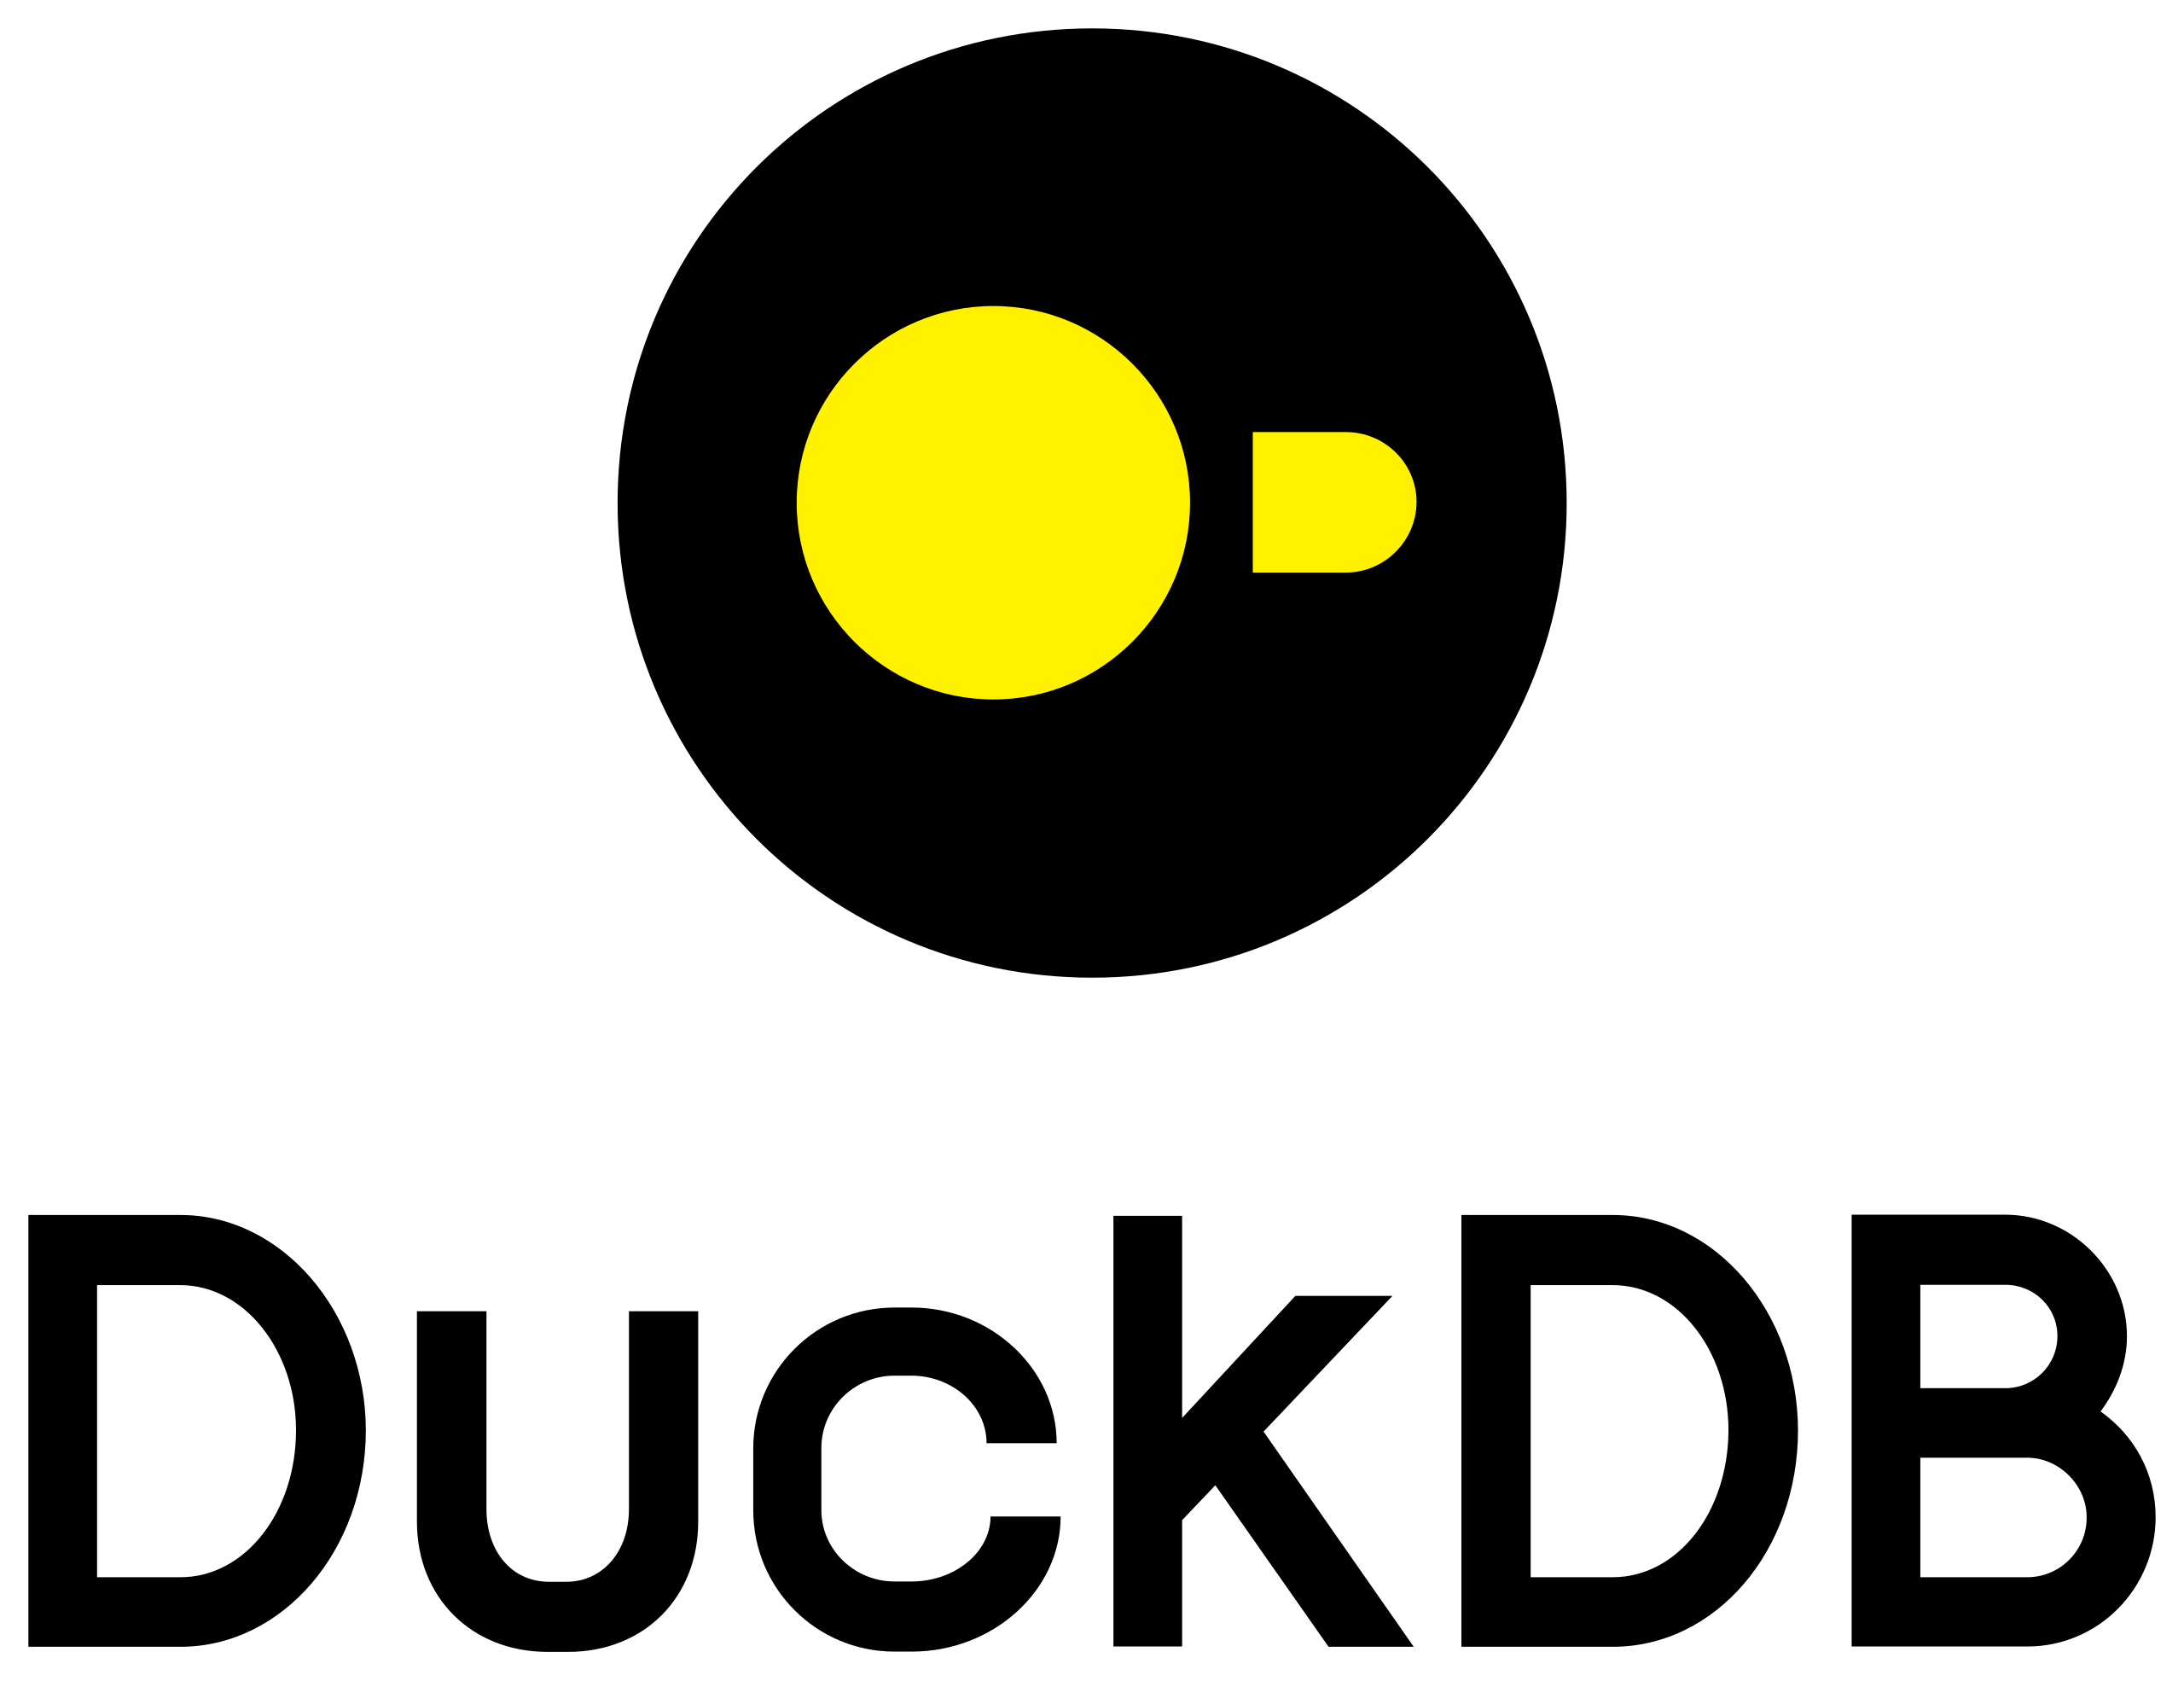
\includegraphics[width=\textwidth]{Images/DuckDB_logo.svg.png}
    \label{fig:duckdb}
  \end{subfigure}
  \hfill
  \begin{subfigure}[b]{0.1\textwidth}
    
\includegraphics[width=\textwidth]{Images/octave.png}
    \label{fig:octave}
  \end{subfigure}
  \hfill
  \begin{subfigure}[b]{0.1\textwidth}
    
\includegraphics[width=\textwidth]{Images/Pandas_logo.svg.png}
    \label{fig:pandas}
  \end{subfigure}

  \par\vspace{1em} % New row with vertical space

  \begin{subfigure}[b]{0.1\textwidth}
    
\includegraphics[width=\textwidth]{Images/ffmpeg.png}
    \label{fig:ffmpeg}
  \end{subfigure}
  \hfill
  \begin{subfigure}[b]{0.1\textwidth}
    
\includegraphics[width=\textwidth]{Images/bash.png}
    \label{fig:bash}
  \end{subfigure}
  \hfill
  \begin{subfigure}[b]{0.1\textwidth}
    
\includegraphics[width=\textwidth]{Images/default_logo.png}
    \label{fig:caengine}
  \end{subfigure}

  \caption{Available Kuspace Applications}
  \label{fig:authservices}
\end{figure}


\subsection{Integration and Security}

Uspace authenticates user actions via JWT tokens issued by the Minioth authentication service. It verifies group memberships and resource permissions using the FsLite metadata store and enforces a Unix-style access control model.

The service is deployed as a Kubernetes \texttt{StatefulSet}, ensuring persistent identity and stable storage across restarts. Uspace stores its embedded database and FsLite metadata in a \texttt{PersistentVolumeClaim} (PVC), ensuring durability of user and job metadata.

Administrators can assign storage volumes, manage user data, inspect system metrics, and access operational logs through authenticated admin endpoints. All internal microservice communications are secured using a shared \texttt{ServiceSecret}, available at runtime to authorized components only.




\newpage



\section{Fslite}

\begin{figure}[h]
  \centering
  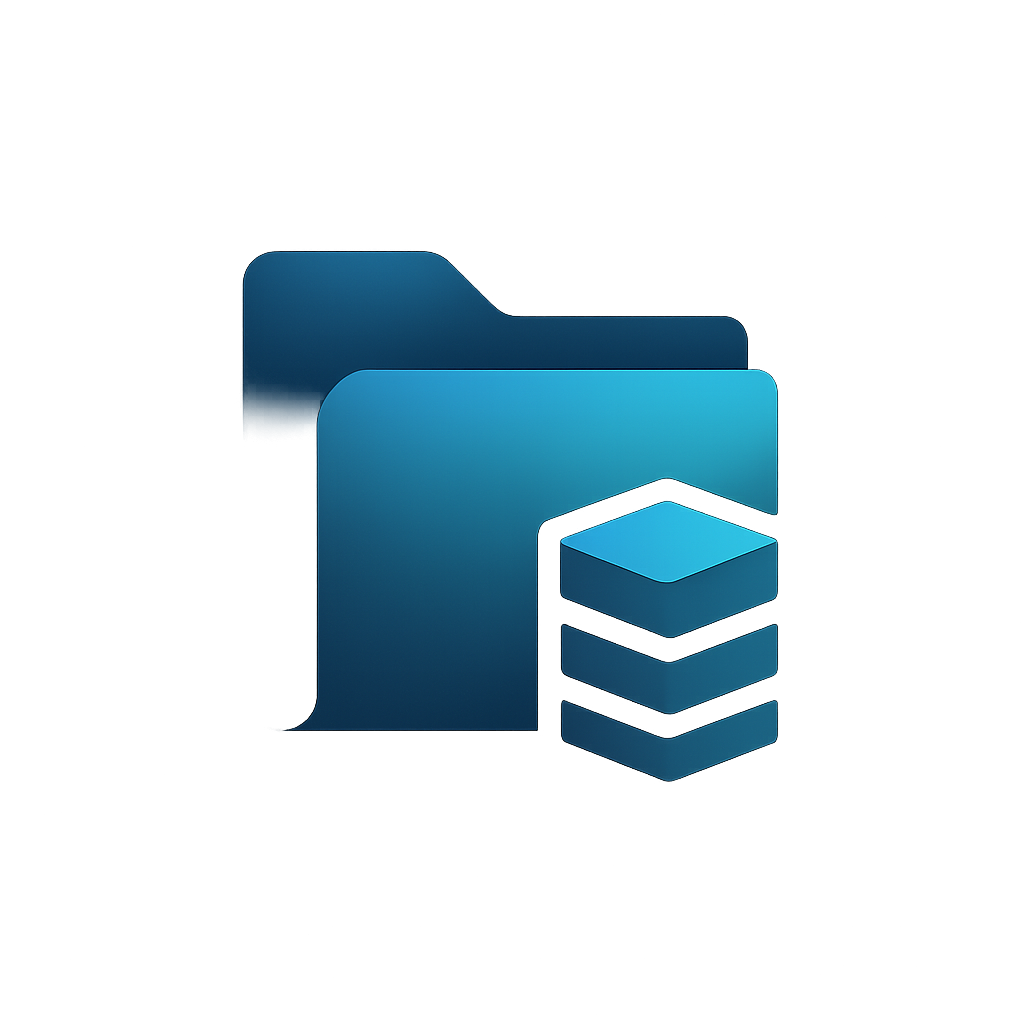
\includegraphics[width=0.3\textwidth]{Images/fslite_chatgpt_draft1.png}
  \caption{FsLite logo}
  \label{fig:fslogo}
\end{figure}


FsLite is a modular metadata and volume management system that can operate either as an embedded library or as a standalone microservice. It is used within the Uspace module to abstract and manage virtual storage concepts, such as user volumes, datasets, and permissions, before interacting with the physical storage backend (MinIO).

\begin{figure}[h!]
  \centering
  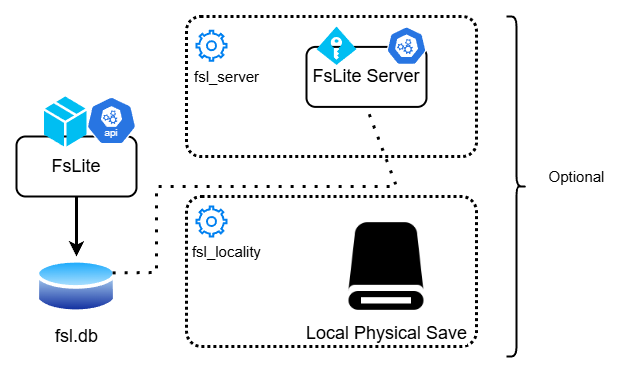
\includegraphics[width=1\textwidth]{Images/fsl.png}
  \caption{FsLite Block Diagram}
  \label{fig:fslite-blockdiagram}
\end{figure}

\subsection{Purpose and Design}

The key design goal of FsLite is to provide a lightweight, configurable system to handle logical resource management, including tracking objects, managing access control, and storing volume definitions. It uses an embedded relational database (SQLite or DuckDB, depending on configuration) for metadata persistence.

FsLite enables the system to:
\begin{itemize}
    \item Create and track logical volumes and resource entries before physical allocation.
    \item Maintain metadata about files, directories, and symbolic links.
    \item Perform access control enforcement based on user and group ownership.
    \item Act as an intermediate layer before delegating large-scale I/O to MinIO.
\end{itemize}

\subsection{Deployment and Initialization}

When deployed in standalone mode, FsLite operates as a RESTful microservice using the Gin web framework. It initializes by connecting to the configured database and optionally preparing a physical volume path on the local filesystem. If enabled, it creates a default volume using the directory and capacity limits specified in the system configuration.

The admin credentials (access and secret key) are inserted during startup. Optionally, the system can bypass authentication for development or local deployments.

\subsection{API Endpoints}

FsLite exposes a structured API grouped under a versioned path. The endpoints are divided into authentication, volume management, and resource operations. Key endpoints include:

\begin{table}[H]
\centering
\resizebox{\textwidth}{!}{%
\begin{tabular}{|l|l|p{9cm}|}
\hline
\textbf{Method} & \textbf{Path} & \textbf{Description}\\
\hline
\hline
POST              & \texttt{/login}                     & Authenticate and receive a token.\\
POST              & \texttt{/admin/register}            & Authenticate and receive JWT token.\\
POST              & \texttt{/admin/volume/new}          & Change password for the authenticated user.\\
DELETE            & \texttt{/admin/volume/delete}       & Delete a specified volume\\
GET               & \texttt{/admin/volume/get}          & Retrieve information about a logical volume\\
GET               & \texttt{/admin/resource/get}        & Retrieve metadata of multiple resources \\ 
GET               & \texttt{/admin/resource/stat}       & Retrieve more detailed metadata of a specific resource.\\
DELETE            & \texttt{/admin/resource/delete}     & Delete a specified resource.\\
POST              & \texttt{/admin/resource/upload}     & Upload resource content to volume.\\
GET               & \texttt{/admin/resource/download}   & Download a resource from storage.\\
GET/PATCH/DELETE  & \texttt{/admin/user/voumes}         & CRUD user volumes.\\
\hline
\hline
\end{tabular}%
}
\caption{FsLite public API endpoints}
\label{tab:fslite-public-endpoints}
\end{table}

\subsection{Integration in the System}

FsLite is integrated into the Uspace module, which delegates resource and volume tracking tasks to it. This modular separation allows Uspace to offload concerns related to volume capacity, ownership verification, and metadata persistence to FsLite.

Its database-backed design allows stateless operation from the perspective of the consuming services. It also enables simulation of filesystem-like permissions using UNIX-style ownership and mode bits.

\subsubsection{Local vs Remote Operation}

FsLite can operate in two modes:
\begin{itemize}
    \item \textbf{Local Mode:} FsLite creates a data directory on the host machine and directly stores uploaded files, suitable for testing or single-node deployments.
    \item \textbf{Remote Mode:} FsLite acts purely as a metadata layer; files are stored in MinIO or other backends using volume references.
\end{itemize}

\begin{figure}[h!]
  \centering
  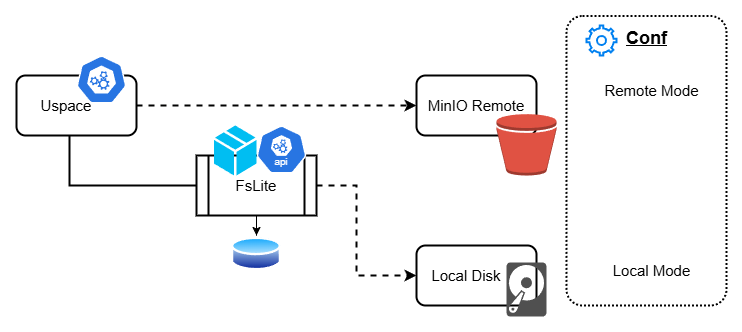
\includegraphics[width=1\textwidth]{Images/fslite-block-diagram.png}
  \caption{FsLite Integration}
  \label{fig:fslite-integration}
\end{figure}



\section{Storage Layer (MinIO)}

MinIO serves as the system's object storage backend, offering a scalable, S3-compatible API for storing and retrieving binary data such as 
uploaded datasets and job output files. It is tightly integrated with Kubernetes and can be accessed from within containers via network mounts 
or HTTP APIs.

Each user’s data is stored under isolated bucket structures or path prefixes, ensuring access control through both object path naming 
conventions and Fslite-based permissions. MinIO's stateless nature and support for erasure coding make it a robust choice for managing large 
data volumes in a distributed environment.

MinIO allows the platform to scale horizontally and reduces the need for traditional shared volumes or file servers. Its integration with 
the rest of the system ensures that users and jobs can read and write data in a uniform and efficient manner.

The MinIO Service is tightly connected to the Uspace Service. Uspace is authorized to perform admin operations on MinIO and also 
allows in its scope the Jobs spawned to fetch and load data to it.

\begin{figure}[h!]
  \centering
  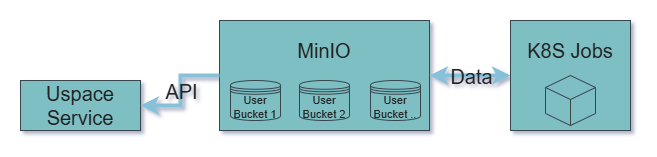
\includegraphics[width=1\textwidth]{Images/minio-overview.png}
  \caption{Minio Service Overview}
  \label{fig:minio-overview}
\end{figure}


MinIO is deployed as a Kubernetes StatefulSet backed by persistent volumes. This ensures durability of user data across pod restarts and facilitates scale-out configurations when needed.

Each service that interacts with MinIO is granted scoped credentials based on service identity. Access control is further enforced using path prefixes aligned with Fslite’s logical resource mappings. The system may optionally use signed URLs for temporary external access to datasets.



\section{Frontend and WebSocket Server}
\label{sec:frontend-wss}

\subsection{Overview}

The Frontend service acts as the primary user interface of the system, offering a web-based environment where users can register, log in, upload datasets, browse their resources, and submit batch analytical jobs. It is implemented using standard web technologies and communicates with backend services via RESTful APIs.

Beyond serving static HTML templates and handling client-side rendering, the Frontend plays a critical role in request mediation. It intercepts client requests, performs sanitization and validation, and attaches authentication tokens or service secrets where necessary. This enables secure and orchestrated communication between the user interface and core backend services, especially the Uspace API.

\subsection{WebSocket Server (WSS)}

The WebSocket Server (WSS) is implemented as a separate microservice that provides real-time, bidirectional communication capabilities between clients and the system. Its primary purpose is to support streaming logs, job status updates, and other event-driven feedback mechanisms related to job execution.

Clients interact with the WSS by issuing HTTP upgrade requests on a dedicated registration endpoint, specifying a Job ID (JID) and their desired role: \textit{Producer}, \textit{Consumer}, or \textit{JackOfAllTrades}. The server internally manages job-specific WebSocket channels. If a connection for the specified JID does not exist, it is initialized; otherwise, the client is added to the existing communication stream.

\begin{table}[H]
\centering
\begin{tabular}{|l|p{10cm}|}
\hline
\textbf{Role} & \textbf{Description} \\
\hline
\texttt{Producer} & Sends messages to the WebSocket channel. Typically used by job execution pods to stream logs, status updates, or results. \\
\texttt{Consumer} & Subscribes to a WebSocket channel and receives messages sent by the associated producer. Ideal for real-time job monitoring. \\
\texttt{JackOfAllTrades} & Can both send and receive messages within the WebSocket channel. Useful for debugging or hybrid clients. \\
\hline
\end{tabular}
\caption{Supported WebSocket communication roles}
\label{tab:wss-roles}
\end{table}


Additionally, an administrative endpoint allows forced disconnection of specific channels or participants, enabling control over job-specific streams.

\begin{figure}[h!]
  \centering
  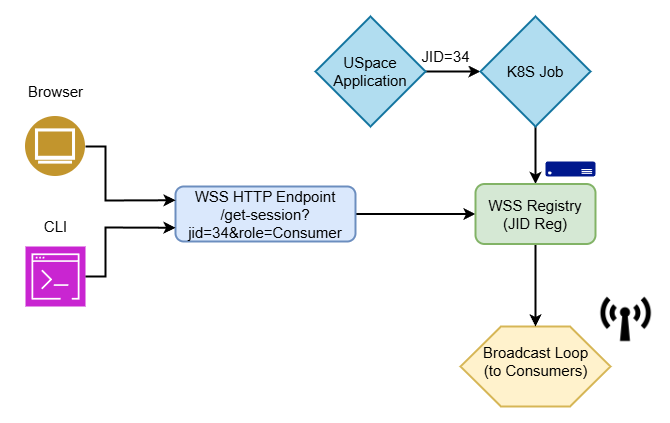
\includegraphics[width=1\textwidth]{Images/wss-blockdriagram.png}
  \caption{Wss Block Diagram}
  \label{fig:wss-blockdiagram}
\end{figure}

\subsection{Frontend–WSS Separation of Concerns}

While both the Frontend and WSS are part of the user-facing layer, they are deployed as independent services with different responsibilities. The Frontend focuses on rendering the user experience and forwarding REST-based job and resource operations to Uspace, while the WSS focuses on real-time feedback for asynchronous job execution.

This separation allows the system to maintain a clear modular boundary between interactive request-response behavior and event-driven streaming, simplifying system maintenance and scaling.


\subsection{Frontend Technology Stack}

The Frontend service is designed to offer a minimal yet responsive user experience, relying on standard web technologies and a server-side rendering model.

\begin{figure}[h!]
  \centering
  \begin{subfigure}[b]{0.15\textwidth}
    
\includegraphics[width=\textwidth]{Images/html.png}
    \label{fig:html5}
  \end{subfigure}
  \hfill
  \begin{subfigure}[b]{0.2\textwidth}
    
\includegraphics[width=\textwidth]{Images/Htmx_Logo.png}
    \label{fig:htmx}
  \end{subfigure}
  \hfill
  \begin{subfigure}[b]{0.1\textwidth}
    
\includegraphics[width=\textwidth]{Images/CSS3_logo_and_wordmark.svg.png}
    \label{fig:css}
  \end{subfigure}

  \begin{subfigure}[b]{0.25\textwidth}
    
\includegraphics[width=\textwidth]{Images/JavaScript-Logo.png}
    \label{fig:javascript}
  \end{subfigure}
  \hfill
  \begin{subfigure}[b]{0.2\textwidth}
    
\includegraphics[width=\textwidth]{Images/Go-Logo_Blue.png}
    \label{fig:golang}
  \end{subfigure}
  \hfill
  \begin{subfigure}[b]{0.15\textwidth}
    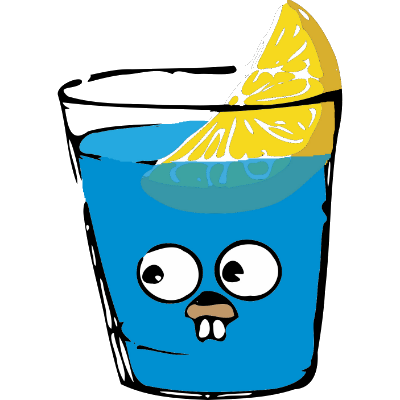
\includegraphics[width=\textwidth]{Images/goGin_Logo.png}
    \label{fig:gogin}
  \end{subfigure}

  \caption{FrontEnd Technologies}
  \label{fig:authservices}
\end{figure}



\begin{itemize}
    \item \textbf{HTMX}~\cite{htmx-docs} is used as the main HTTP client, enabling dynamic content updates by issuing declarative AJAX requests embedded in HTML attributes. This reduces the need for complex JavaScript frameworks.
    
    \item \textbf{Go Templates} render HTML pages server-side using Go’s \texttt{html/template} engine. This allows safe and dynamic construction of views tied directly to backend logic.
    
    \item \textbf{Vanilla JavaScript} is used for basic DOM manipulation, file previews, and UI behaviors. The system avoids heavy client-side frameworks to maintain performance and reduce complexity.
    
    \item \textbf{CSS} is used to apply styling and layout. The design aims for clarity and usability, with lightweight responsive behavior for handling multiple screen sizes.
    
    \item \textbf{Gin Framework} in Go powers the backend of the Frontend service, handling routing, middleware, and template rendering.
\end{itemize}

Security is enforced via JWT-based middleware and service-to-service secret headers. All critical interactions (e.g., job submissions, resource uploads) are protected with authentication and validated on the server.

\begin{figure}[h!]
  \centering
  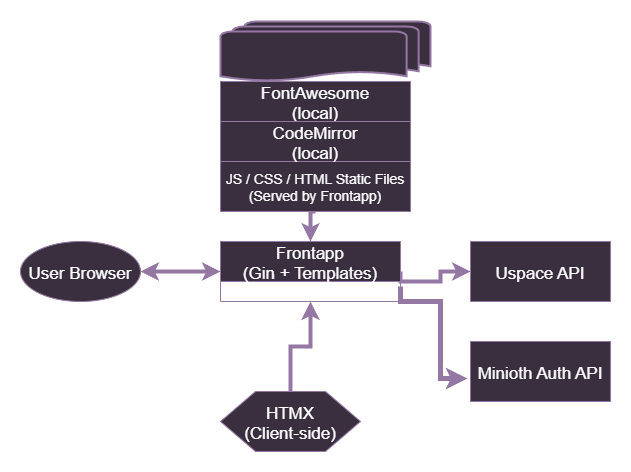
\includegraphics[width=1\textwidth]{Images/frontapp-blockdiagram.png}
  \caption{Frontapp Overview diagram}
  \label{fig:frontapp-overview}
\end{figure}

To support syntax-highlighted editing for user-submitted scripts (e.g., SQL, Python), the frontend integrates CodeMirror, a versatile in-browser code editor~\cite{codemirror}.

Interface icons, tool indicators, and status badges are rendered using the Font Awesome Free icon library~\cite{fontawesome}, providing visual consistency and accessibility.
Both technology stacks are served from Frontapp, bypassing any cdn.

\subsection{Integration}
Both the Frontapp and the Wss are integrated in the system as Kubernetes Deployments remaining stateless. There is also ephimeral logging, 
which can be used in the future.



\section{Kubernetes Integration}

Kubernetes functions as the orchestration backbone of the system. It is responsible for deploying, scheduling, and executing containerized jobs 
submitted by users. Uspace leverages Kubernetes Jobs to launch sandboxed environments in which user-specified tools (e.g., DuckDB, Octave) are 
executed. It also deployes each Microservice itself, tightening overall security and exposes only the desired service to the end user. In 
this case everything should be used and accessed via Frontapp.

Additionally, Kubernetes' Persistent Volume Claims (PVCs) or object storage access is used in allignment with StatefulSets to persist data. 
Everything deployed on K8S is namespaced. 

Each service is included with a Kubernetes Service and configured accordingly so that there is inter-service communication. There is also use 
for Node-Port Services for the system entrypoints.

Overall, the integration with Kubernetes allows the system to inherit properties such as fault tolerance, scaling, and container lifecycle management. 
It enables infrastructure-level abstraction so that users do not need to interact directly with Kubernetes primitives.
% Todo

\chapter{System Usage \& Execution Flow}
\section{Deployment and Tooling}

This section outlines how the system is deployed, the development tools used 
throughout the implementation, and the underlying infrastructure model.

\subsection{Deployment Procedure}

The system is built to run on Kubernetes, with support for local development and testing via Minikube and Docker Desktop. While it has not been extensively validated on production-grade Kubernetes clusters, all features and microservices operate successfully in local Kubernetes environments.

Deployment is orchestrated using a dedicated Go-based tool named kuspacectl.go. This CLI tool simplifies building, deploying, and tearing down the entire stack. It handles:

\begin{itemize}
\item Building Docker images for each microservice.
\item Creating or destroying the Kubernetes namespace \texttt{kuspace}.
\item Applying all Kubernetes manifests found under the 
\texttt{/deployment/kubernetes} directory.
\item Generating secrets and initial configurations.
\end{itemize}

In addition to kuspacectl, traditional Makefiles are available to facilitate tasks such as code building, static analysis, cleaning, documentation generation, and running unit tests.

The development process incorporates:

\begin{itemize}
\item \textbf{Golang} with modules for all backend microservices.
\item \textbf{golangci-lint}~\cite{golangcilint} for linting and static analysis.
\item \textbf{go test} for unit and integration testing.
\item \textbf{Swagger}~\cite{swagger} documentation generation for HTTP APIs.
\item \textbf{Golds}~\cite{golds} for Golang documentation generation.
\item \textbf{Air}~\cite{air} for live hot reload in Go apps/services. Used mostly for the Frontapp development.
\item \textbf{AI Assistance Tools}: During development and refinement, AI-assisted code review and language 
models (e.g., ChatGPT) were used to prototype logic, validate syntax, and improve structural clarity. 
These tools were used judiciously, with all code and documentation critically evaluated and verified by 
the author.
\end{itemize}

\subsection{Infrastructure Overview}

The deployment manifests are defined in the \texttt{/deployment/kubernetes} directory. This includes the full Kubernetes configuration for each service:

\begin{itemize}
\item \textbf{Namespaces:} All resources are grouped under the \texttt{kuspace} namespace.
\item \textbf{ConfigMaps:} Service-specific configuration values, including environment variables and runtime parameters.
\item \textbf{Secrets:} Secure key material such as JWT signing secrets and service authentication keys.
\item \textbf{Deployments \& StatefulSets:} Stateless services (like the Frontend) use \texttt{Deployment} 
objects, while stateful components (like \texttt{Minioth} and \texttt{Uspace}) are defined as \texttt{StatefulSets} 
with persistent volume claims (PVCs).
\item \textbf{Services:} ClusterIP services are exposed internally for inter-service communication, 
while the Frontend may optionally be exposed externally.
\end{itemize}

The system architecture encourages modularity and scalability. All microservices are independently containerized and can be redeployed or scaled individually.




\section{System Access and Communication}
\subsection{Access Points and Interfaces}

The system is primarily designed to be accessed through the web-based \texttt{Frontapp} user interface, 
which provides a convenient entry point for typical end-users. However, developers or system integrators 
can interact directly with the backend services via command-line tools or custom HTTP clients, such as 
\texttt{curl}, \texttt{httpie}, or language-specific libraries.

All core services expose their functionality over RESTful APIs. These APIs are documented using Swagger 
(OpenAPI), with each service providing a dedicated endpoint for live exploration and testing (e.g., 
\texttt{/swagger/index.html}). These interfaces offer comprehensive descriptions of all available routes, 
expected parameters, response structures, and authorization requirements.

\subsection{Request-Response Model}

Communication with the backend services follows the standard HTTP request-response model. Beyond typical 
REST conventions, several HTTP headers are critical for correct operation:

\begin{itemize}
    \item \texttt{Authorization}: Contains the Bearer token issued by the authentication service (\texttt{Minioth}). This token encodes the user ID, group membership, and role, and is required for all authenticated actions.
    
    \item \texttt{X-Service-Secret}: Used to authenticate requests between microservices or to authorize trusted developer actions. Each internal service shares a secret key that validates privileged operations.
    
    \item \texttt{Access-Target}: A custom header required by the \texttt{Uspace} service. It encodes both the target of the action (volume ID, resource path) and the identity context (user ID, group IDs) to enforce resource-level authorization. Its format follows:
    
    \begin{quote}
    \texttt{<volume\_id>:<volume\_name>:<resource\_path> <user\_id>:[group\_id,group\_id,\ldots]}
    \end{quote}
    
    This design allows \texttt{Uspace} to separate identity verification (via JWT) from fine-grained access control at the resource level.
\end{itemize}

\subsection{Error Handling and Feedback}

Each microservice is responsible for validating input, authenticating requests, and returning appropriate 
error codes and messages using standard HTTP status codes (e.g., \texttt{401 Unauthorized}, 
\texttt{403 Forbidden}, \texttt{404 Not Found}, \texttt{500 Internal Server Error}).

On the frontend, the \texttt{Frontapp} uses HTMX event hooks to capture responses and dynamically update the user interface. Errors are caught and displayed as user-friendly feedback elements, while success events trigger content refreshes, loading indicators, or UI transitions. This approach enhances responsiveness and usability without relying on full client-side frameworks.



\section{End-to-End Workflow}
\subsection{Overview and User Roles}

Currently there is only a distinction between admins and users. Admins are the users that bear the \textbf{admin} role.
Every new registered user is simply a regular user. Admins can edit and promote other users to admins, by simply 
giving them the \textbf{admin} group.

There is a plan to incorporate the \textbf{mod} (moderator) group which will grant users more privileges than 
regular users but fewer than admins.

\begin{figure}[!htbp]
  \centering
  \begin{subfigure}[b]{0.48\textwidth}
    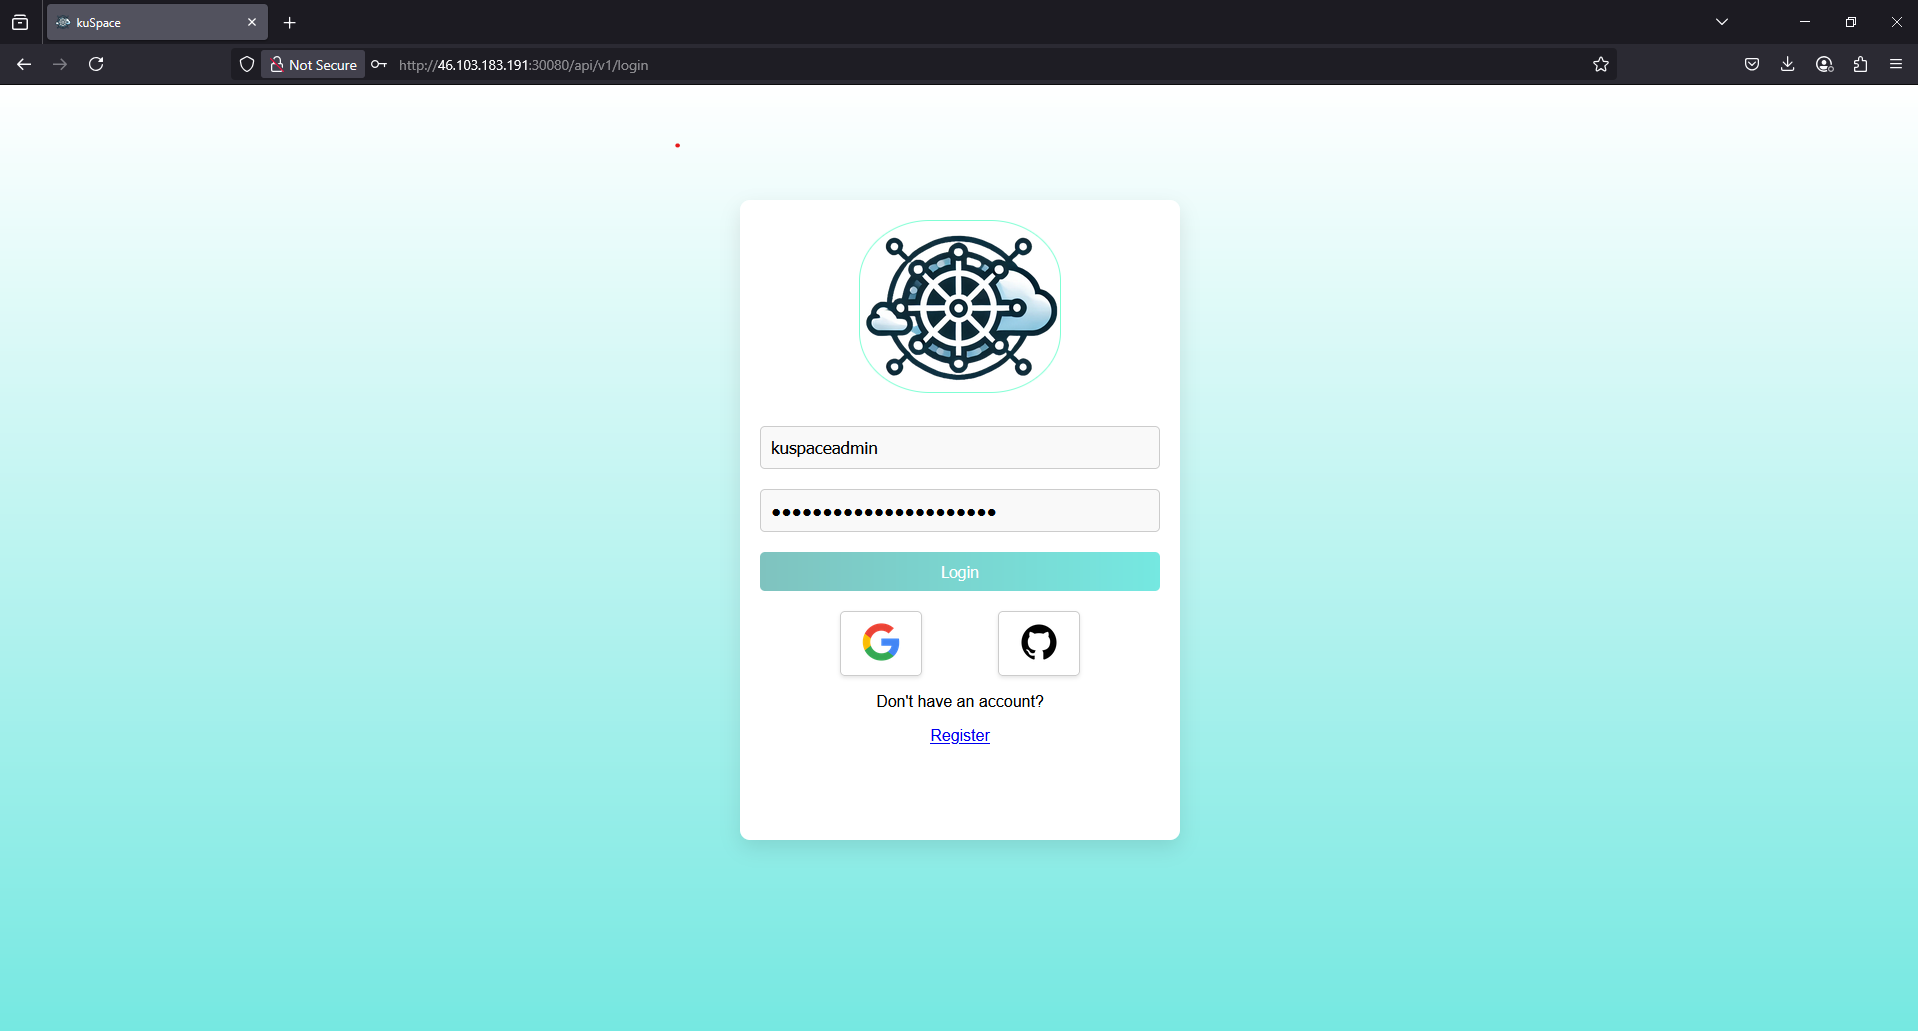
\includegraphics[width=\textwidth]{Images/kuspace_login-page.png}
    \caption{Login Page}
    \label{fig:login}
  \end{subfigure}
  \hfill
  \begin{subfigure}[b]{0.48\textwidth}
    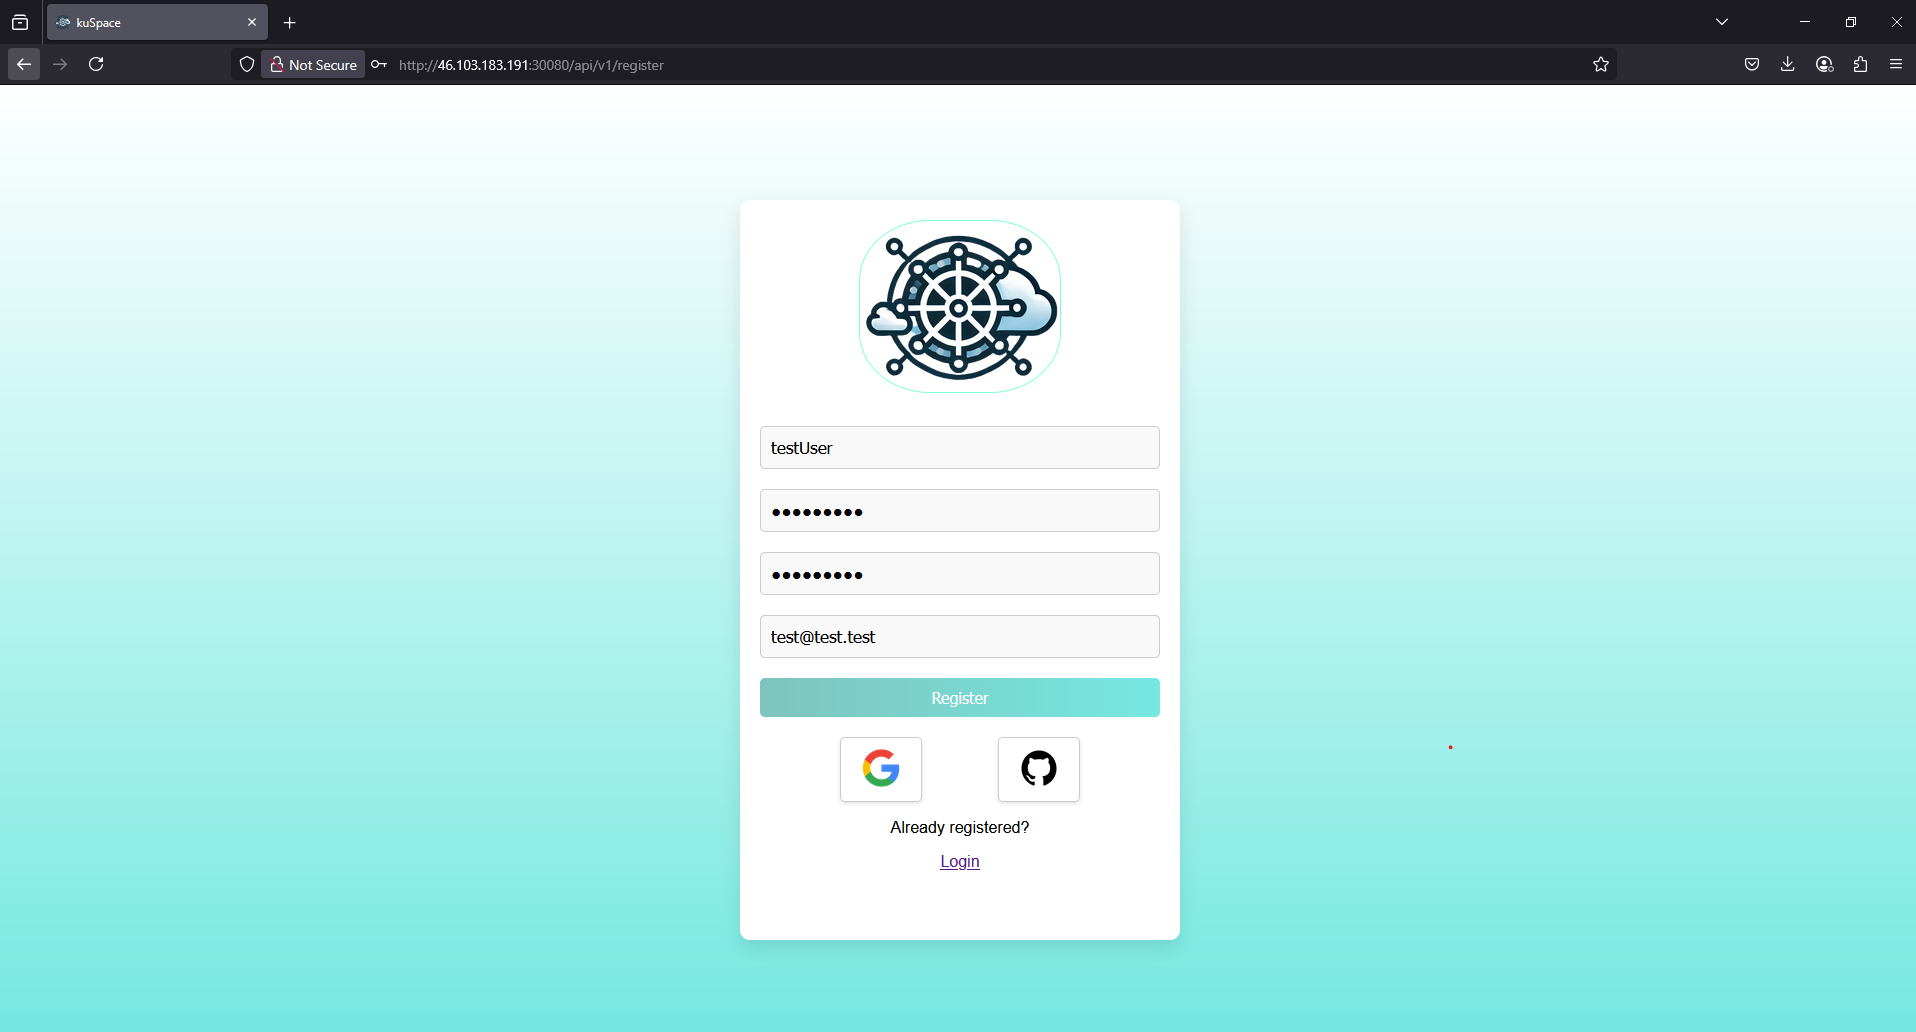
\includegraphics[width=\textwidth]{Images/kuspace_register-page.png}
    \caption{Register Page}
    \label{fig:register}
  \end{subfigure}
  \caption{Kuspace Login and Register Pages}
  \label{fig:authservices}
\end{figure}



The OAuth by Google and Github structure is implemented, yet not fully functional at this point.

There are restrictions on user registration: passwords must match, meet a minimum length, and contain a variety of character types.
Usernames are also constrained by minimum and maximum length requirements, and certain names are prohibited.
\newpage

\subsection{User Perspective}

\begin{figure}[!htbp]
    \centering
    % First row - two side-by-side
    \begin{subfigure}[b]{0.48\textwidth}
        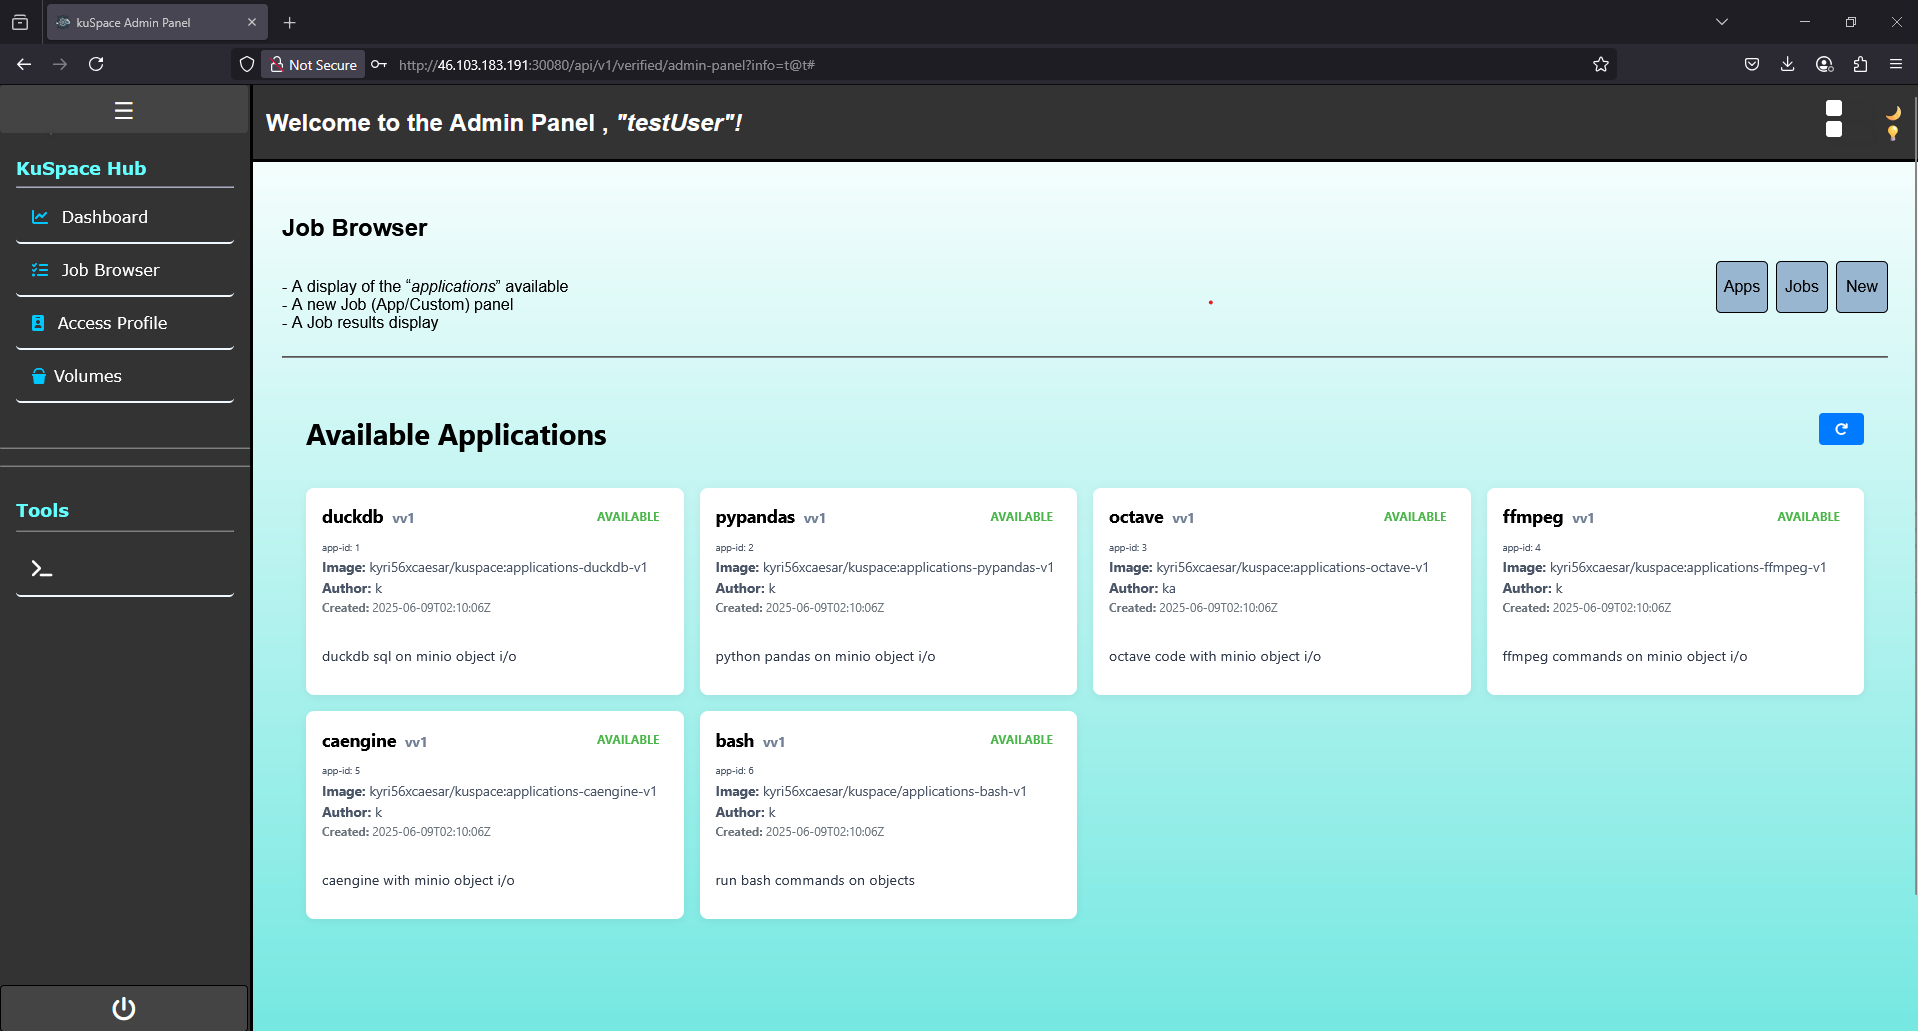
\includegraphics[width=\textwidth]{Images/kuspace_user_jobBrowser_apps.png}
        \caption{Job Browser and App Selection}
        \label{fig:jobbrowserapps}
    \end{subfigure}
    \hfill
    \begin{subfigure}[b]{0.48\textwidth}
        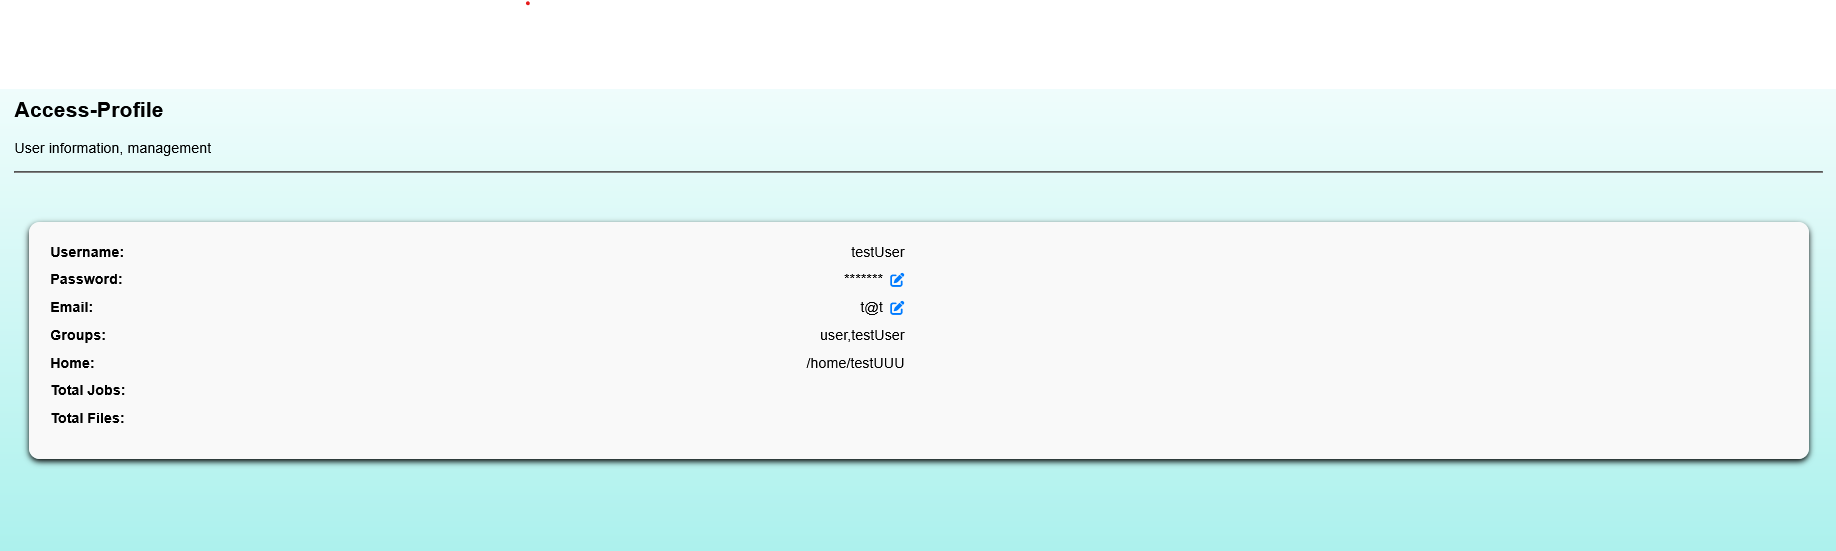
\includegraphics[width=\textwidth]{Images/kuspace_user_accessInfo_change.png}
        \caption{Access Info and Change View}
        \label{fig:accessinfochange}
    \end{subfigure}

    \vspace{1em}

    % Second row - full width
    \begin{subfigure}[b]{0.98\textwidth}
        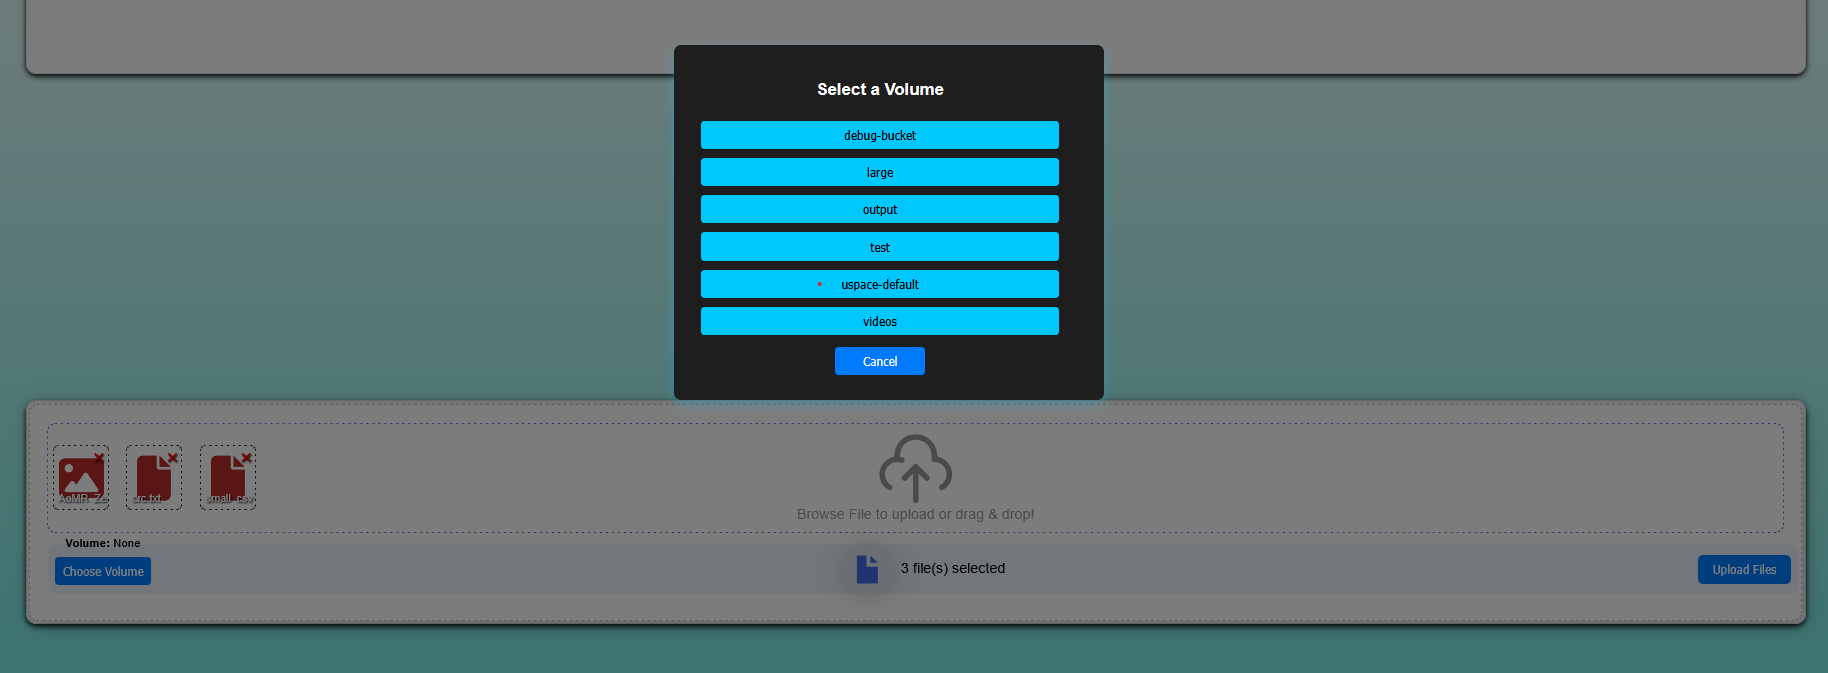
\includegraphics[width=\textwidth]{Images/kuspace_user_fileUploadVolumeChoice.png}
        \caption{File Upload with Volume Selection}
        \label{fig:fileuploadvolume}
    \end{subfigure}

    \caption{User Interface Actions in Kuspace}
    \label{fig:useractions}
\end{figure}

Here we can see the agency a user has to change his credentials, upload files on existing volumes 
and see the available applications. 

\newpage
\begin{figure}[!htbp]
    \centering
    \begin{subfigure}[b]{0.48\textwidth}
        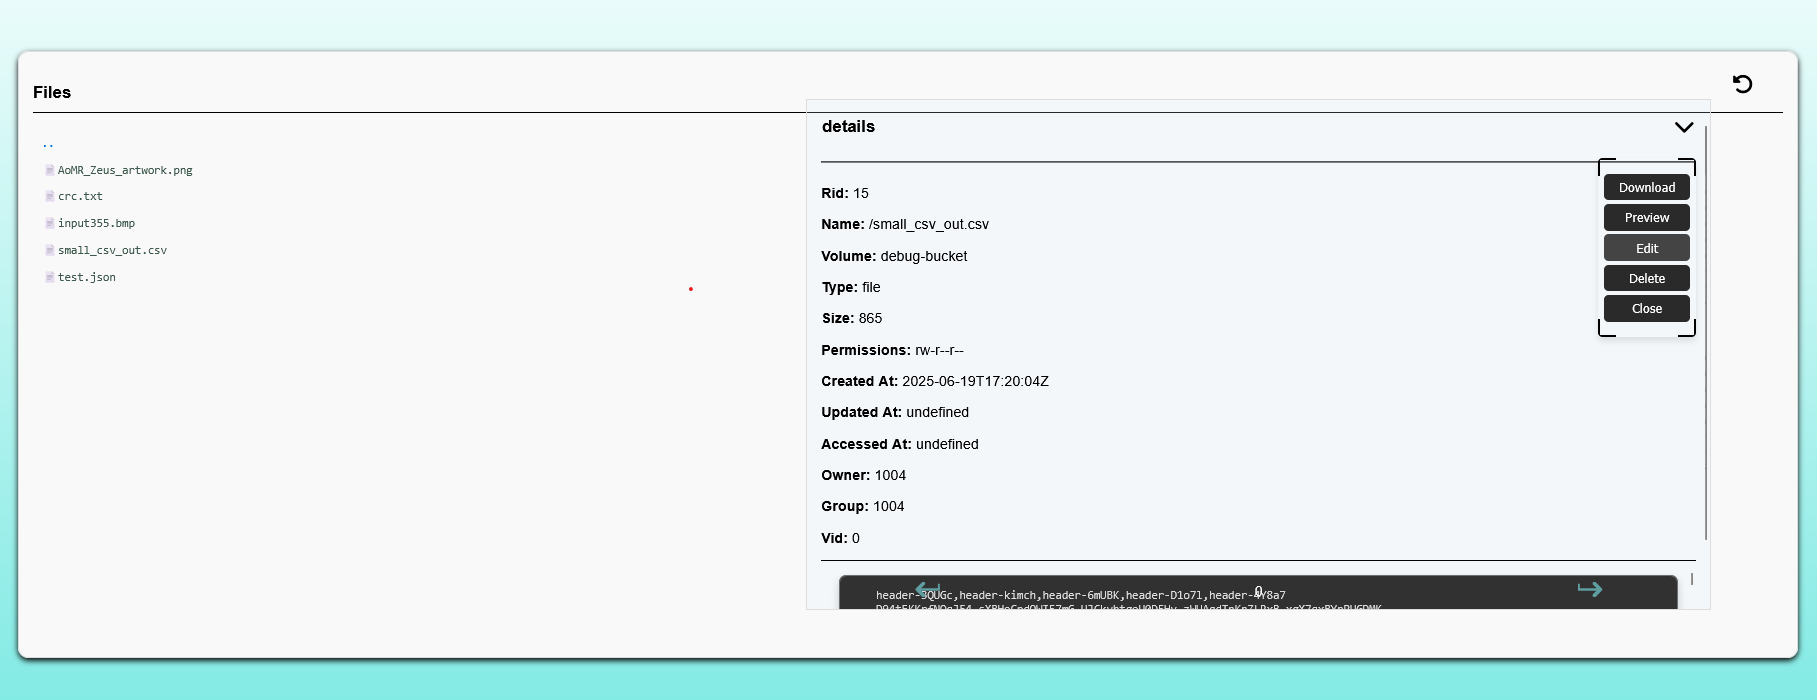
\includegraphics[width=\textwidth]{Images/kuspace_user_fileTraversanlOptions.png}
        \caption{File Traversal and Options}
        \label{fig:filetraversal}
    \end{subfigure}
    \hfill
    \begin{subfigure}[b]{0.48\textwidth}
        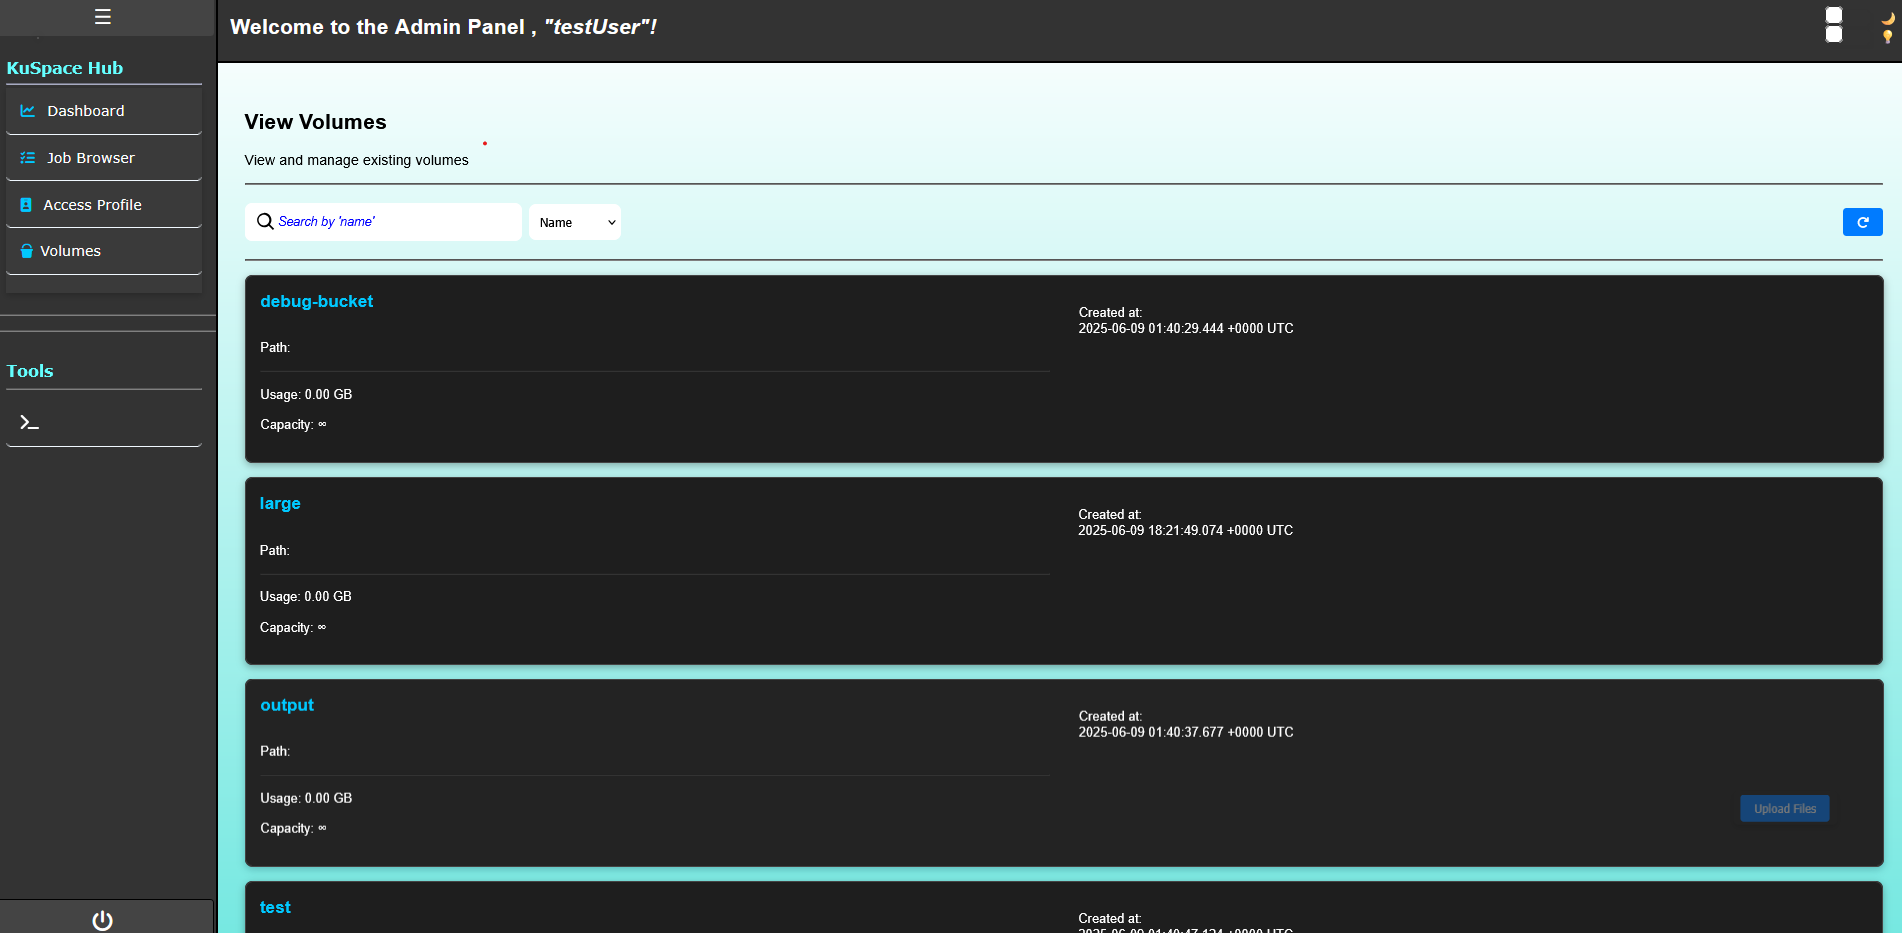
\includegraphics[width=\textwidth]{Images/kuspace_VolumeView.png}
        \caption{Volume Overview}
        \label{fig:volumeview}
    \end{subfigure}
    \caption{Kuspace user views for navigating files and inspecting volumes.}
    \label{fig:user-file-volume}
\end{figure}

\vspace{0.5em}
\noindent
These interfaces allow users to browse directories, inspect resources, and 
understand volume boundaries within the system. Navigation tools and volume 
metadata views help contextualize jobs and uploaded files.


\newpage
\begin{figure}[!htbp]
    \centering
    \begin{subfigure}[b]{0.48\textwidth}
        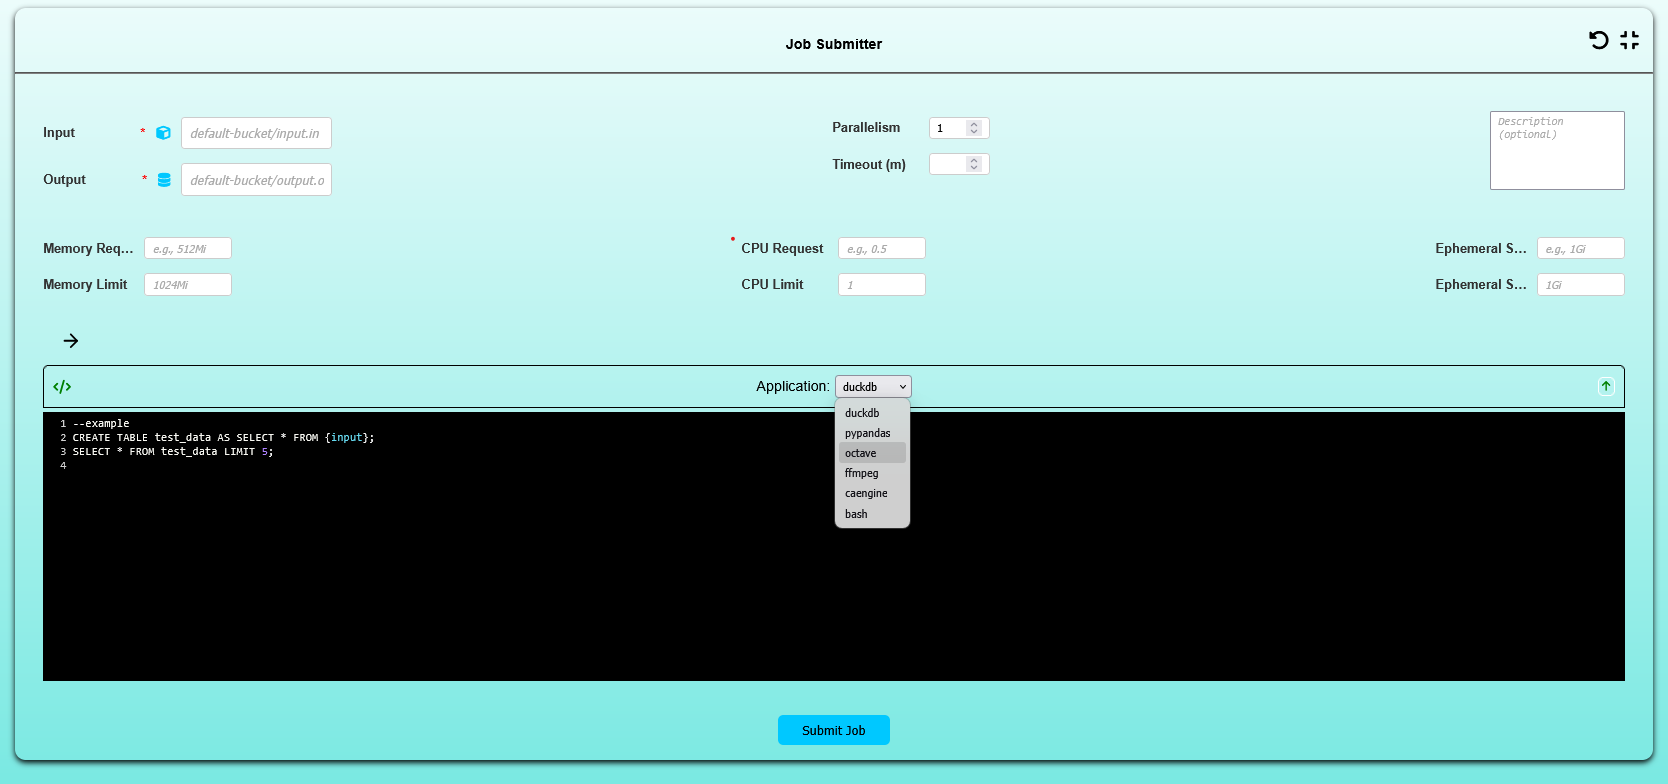
\includegraphics[width=\textwidth]{Images/kuspace_jobSubmitter.png}
        \caption{Job Submitter Panel}
        \label{fig:jobsubmitter}
    \end{subfigure}
    \hfill
    \begin{subfigure}[b]{0.48\textwidth}
        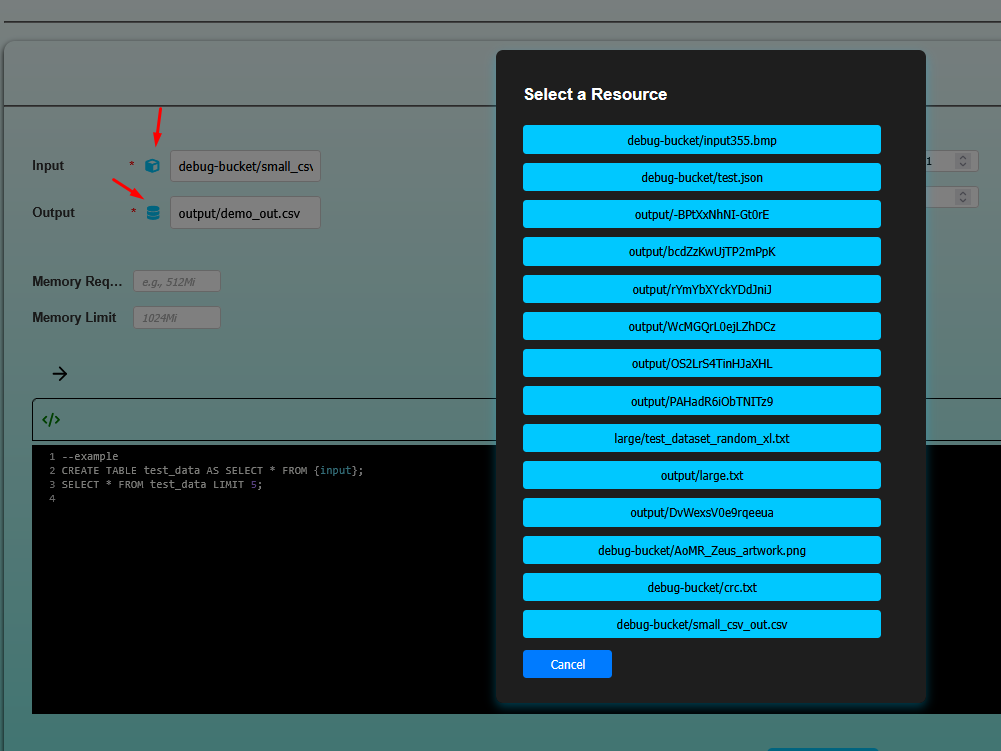
\includegraphics[width=\textwidth]{Images/kuspace_jobSubmitter_selectIO.png}
        \caption{Input/Output Selection}
        \label{fig:jobsubmitterselect}
    \end{subfigure}

    \vspace{1em}

    \begin{subfigure}[b]{0.48\textwidth}
        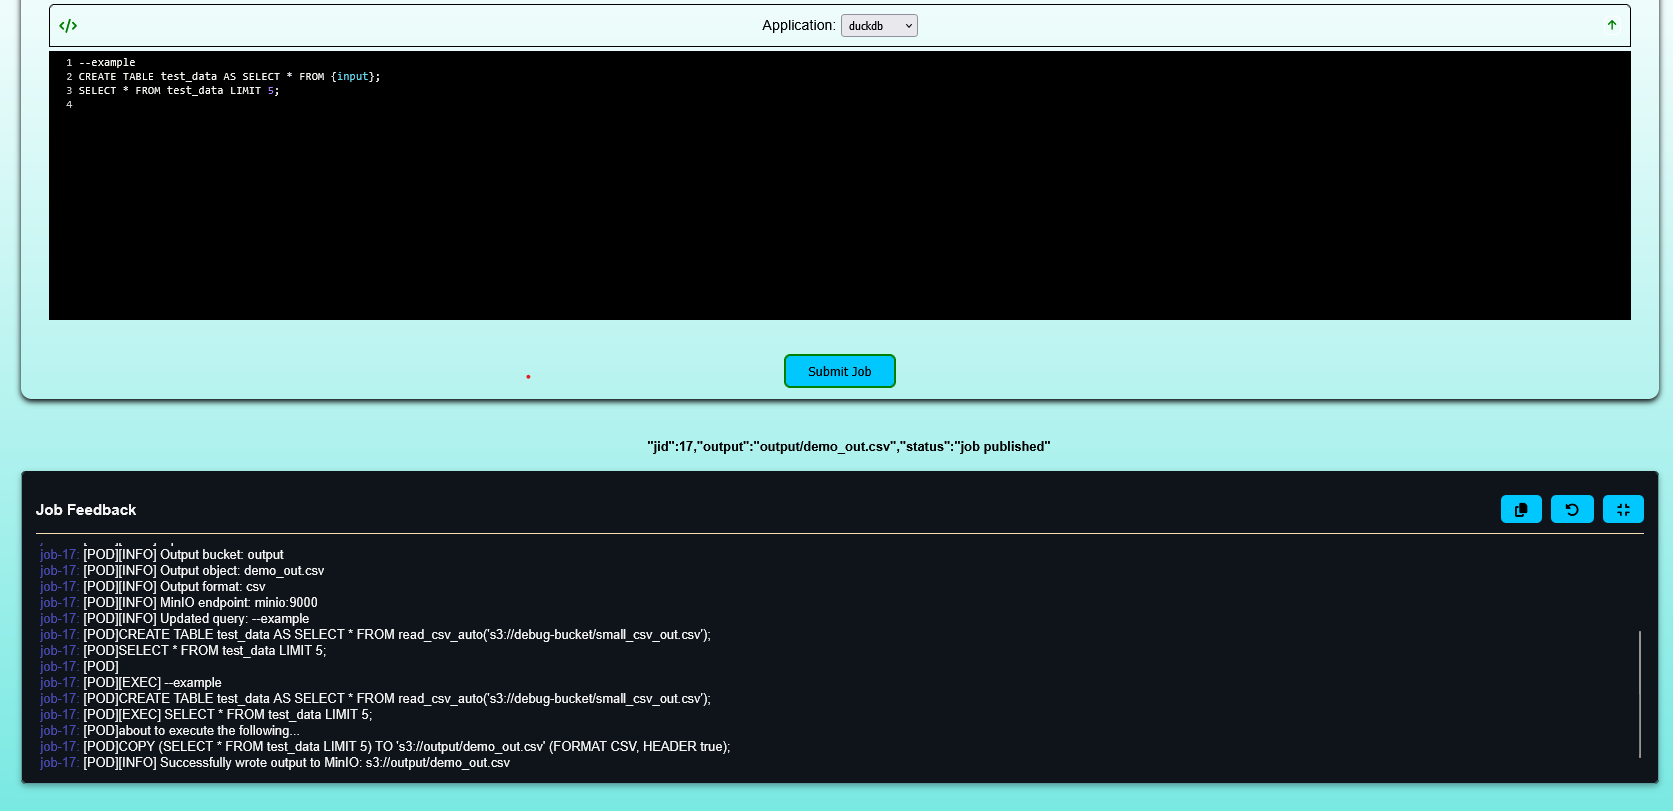
\includegraphics[width=\textwidth]{Images/kuspace_jobSubmission_test.png}
        \caption{Job Published \& Execution Streaming}
        \label{fig:jobsubmission}
    \end{subfigure}
    \hfill
    \begin{subfigure}[b]{0.48\textwidth}
        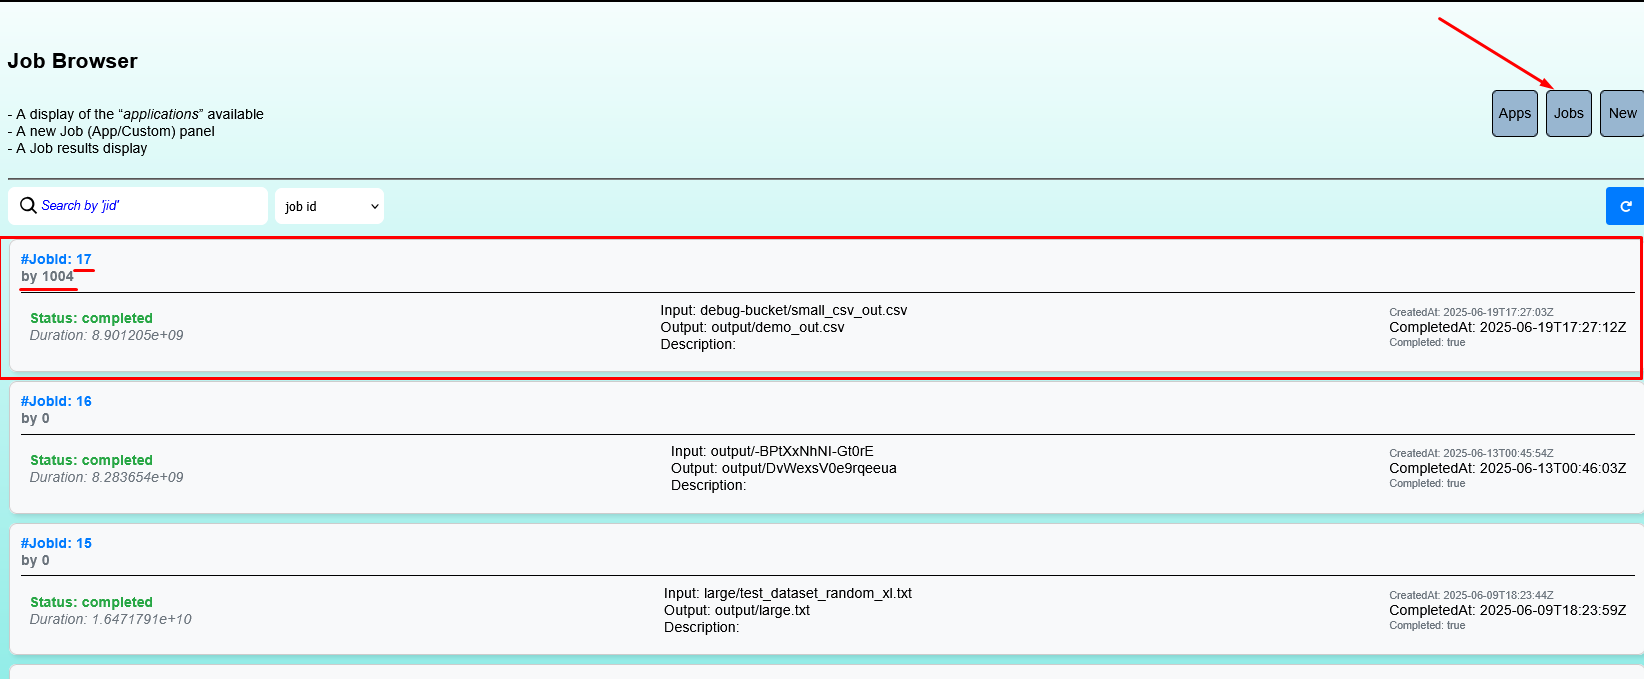
\includegraphics[width=\textwidth]{Images/kuspace_jobView.png}
        \caption{Job Execution Results}
        \label{fig:jobview}
    \end{subfigure}

    \caption{Kuspace user interface for submitting jobs.}
    \label{fig:kuspacejobflow}
\end{figure}

\vspace{0.5em}
\noindent
The workflow includes selecting an application, 
specifying input/output paths, tuning job parameters, 
and viewing results.


\newpage

\subsection{Admin Perspective}
Kuspace advanced administrative actions, including job mutation and system configuration view. 
These tools help define volumes, manage jobs, and manage resource properties.
These views allow administrators to control access and maintain structure.

There are also stylistic options, for example dark-mode, and less verbosity in the top right corner.

\begin{figure}[!htbp]
    \centering
    \begin{subfigure}[b]{0.48\textwidth}
        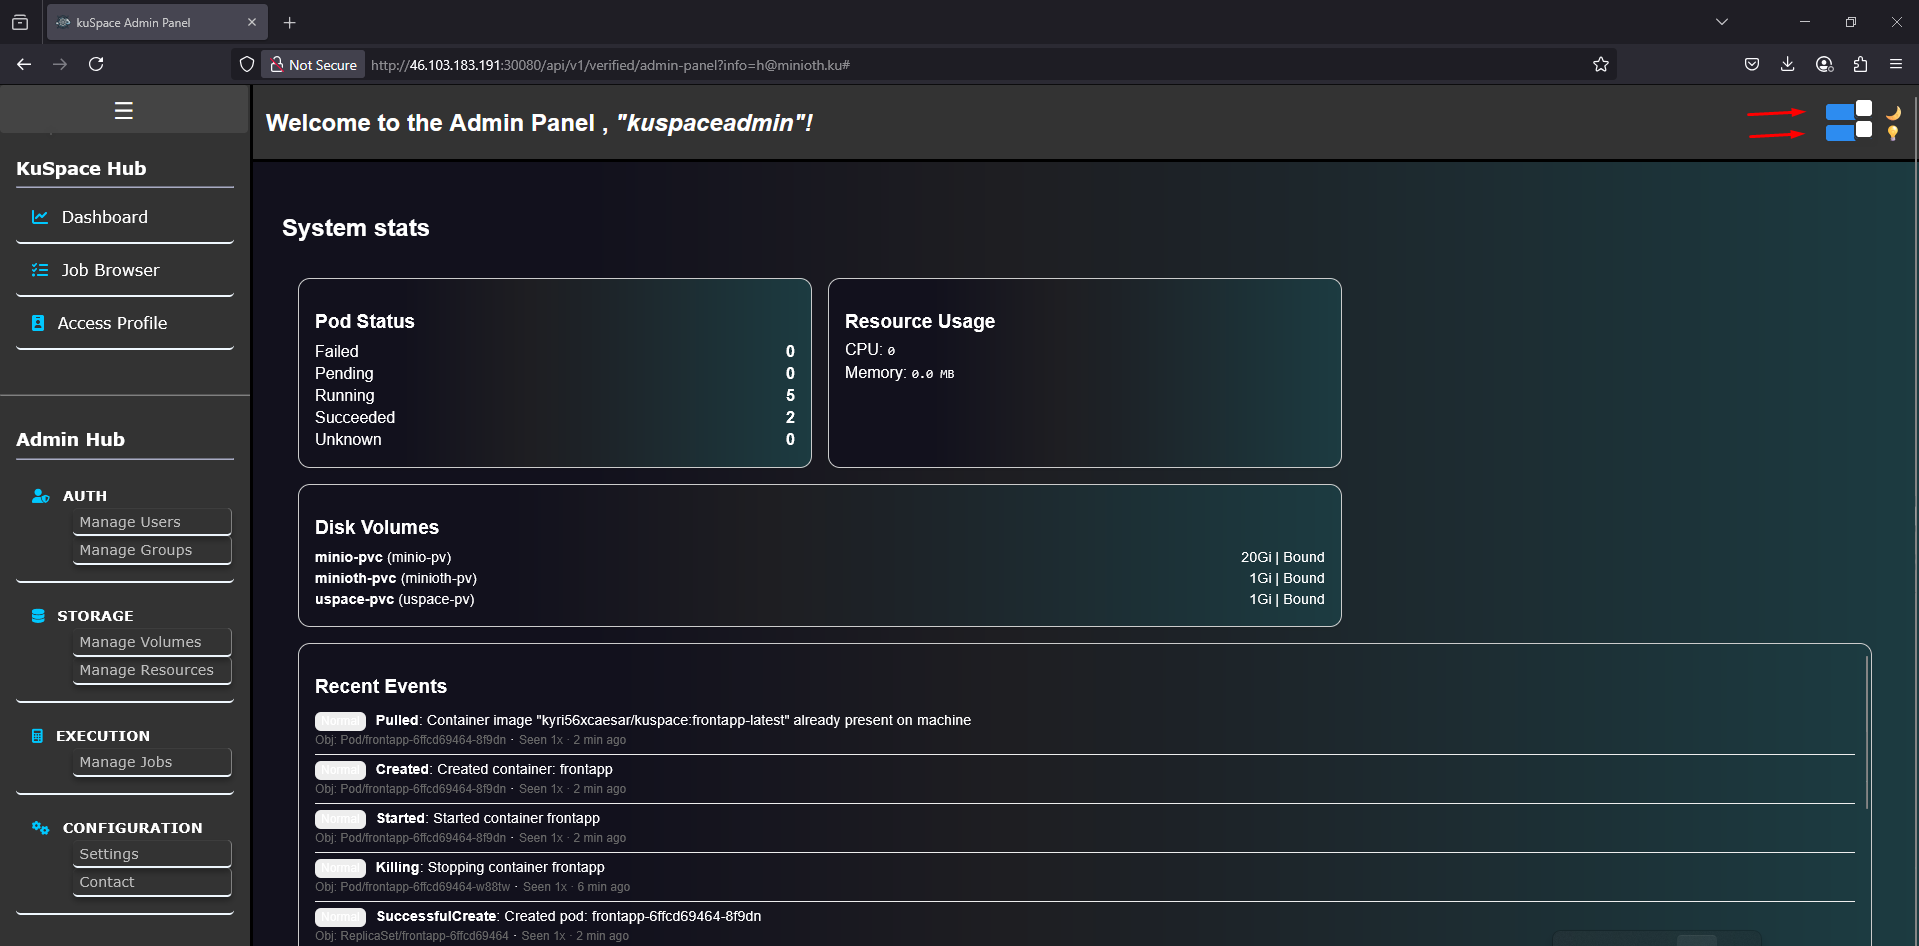
\includegraphics[width=\textwidth]{Images/kuspace_adminDashboard.png}
        \caption{Admin Dashboard Overview}
        \label{fig:adminviewdashboard}
    \end{subfigure}
    \hfill
    \begin{subfigure}[b]{0.48\textwidth}
        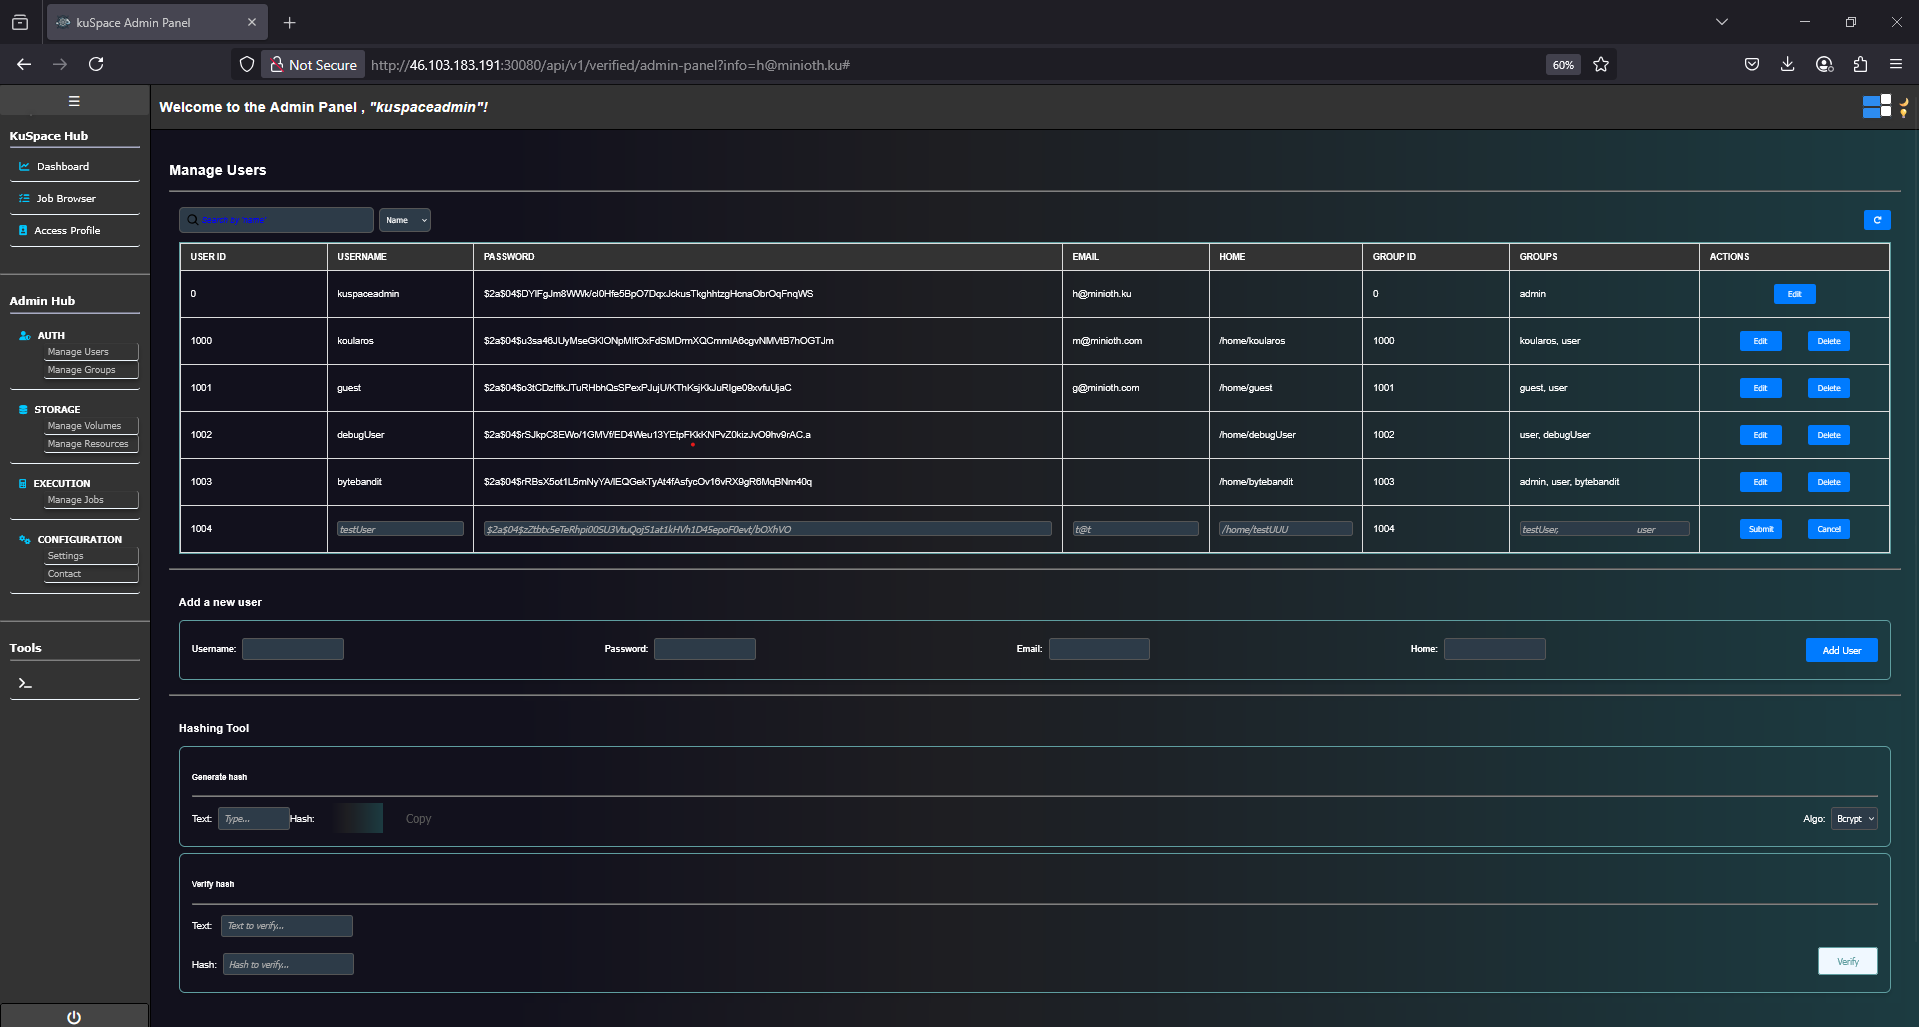
\includegraphics[width=\textwidth]{Images/kuspace_admin_ManageUsers.png}
        \caption{User Management Panel}
        \label{fig:adminmanageusers}
    \end{subfigure}

    \vspace{1em}

    \begin{subfigure}[b]{0.48\textwidth}
        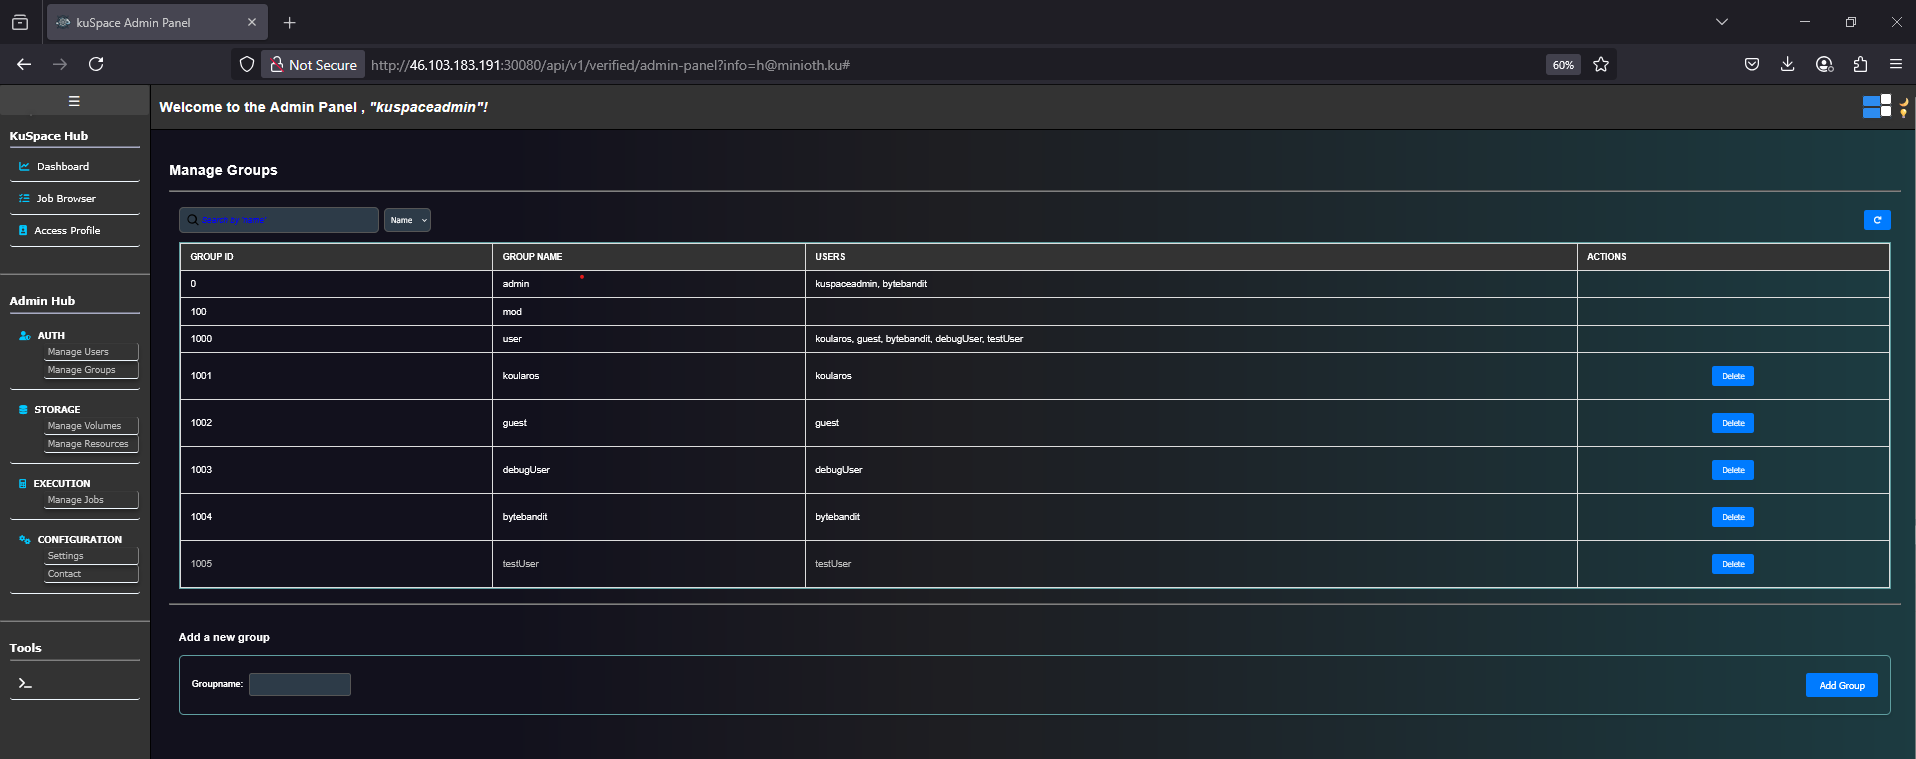
\includegraphics[width=\textwidth]{Images/kuspace_admin_ManageGroups.png}
        \caption{Group Management}
        \label{fig:adminmanagegroups}
    \end{subfigure}
    \hfill
    \begin{subfigure}[b]{0.48\textwidth}
        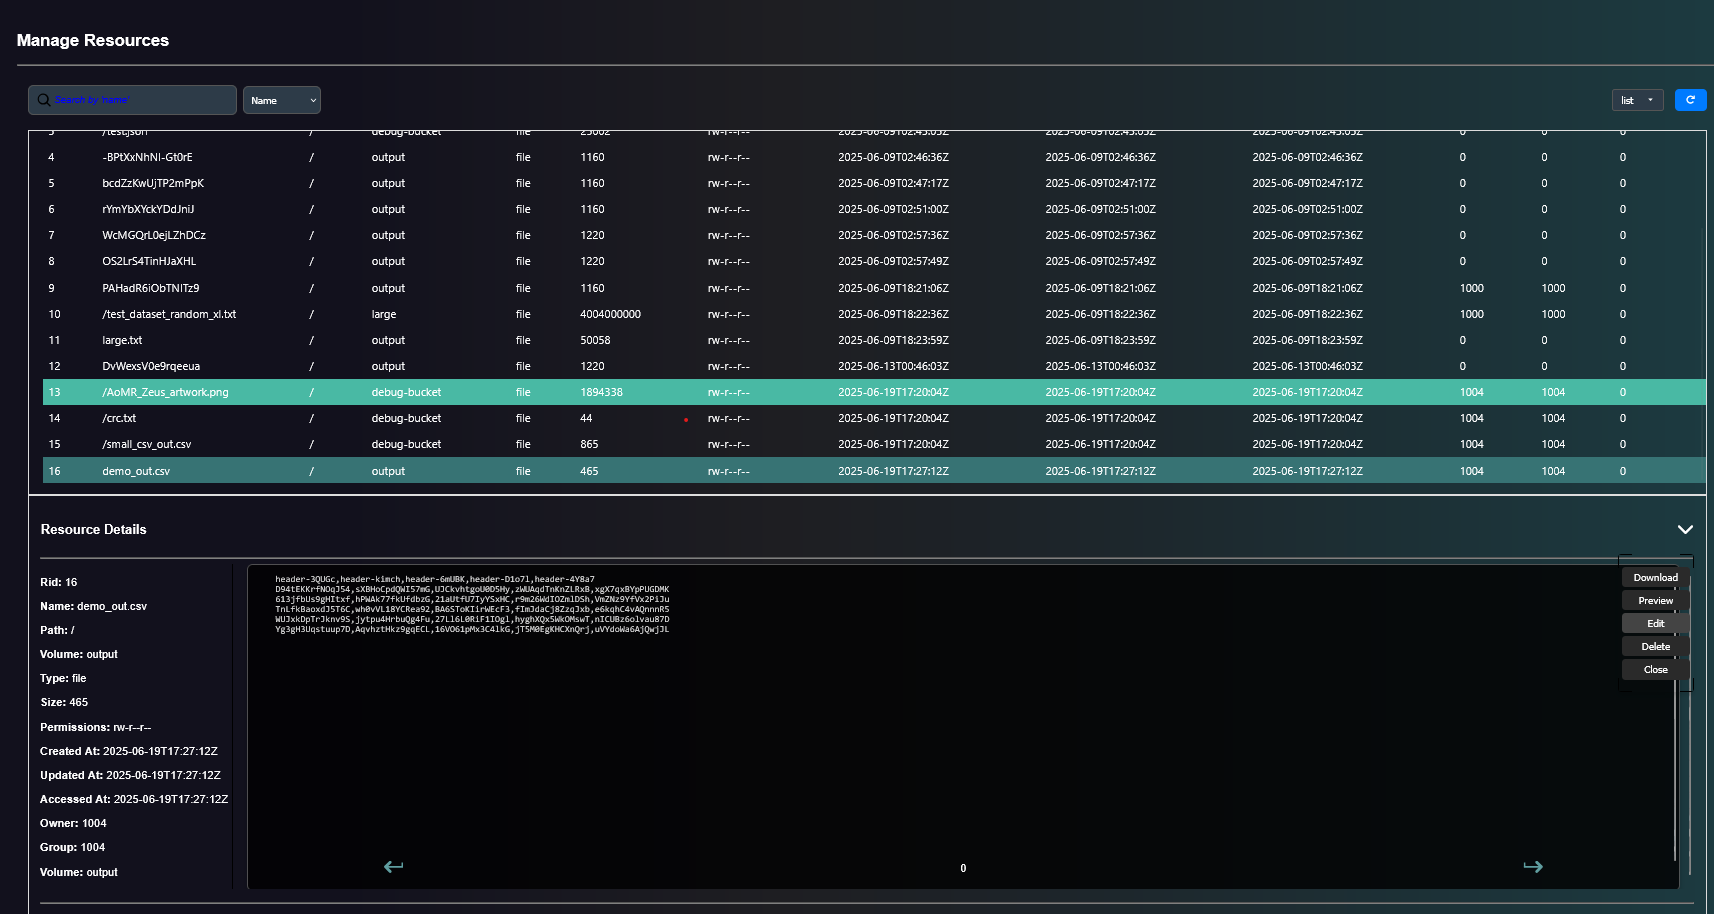
\includegraphics[width=\textwidth]{Images/kuspace_admin_ManageResources.png}
        \caption{Resources Management}
        \label{fig:adminmanageresources}
    \end{subfigure}

    \caption{Kuspace admin interface for managing users, groups, and resources.}
\end{figure}
\vspace{0.5em}
\noindent

\vspace{1em}

\begin{figure}[!htbp]
    \centering
    \begin{subfigure}[b]{0.48\textwidth}
        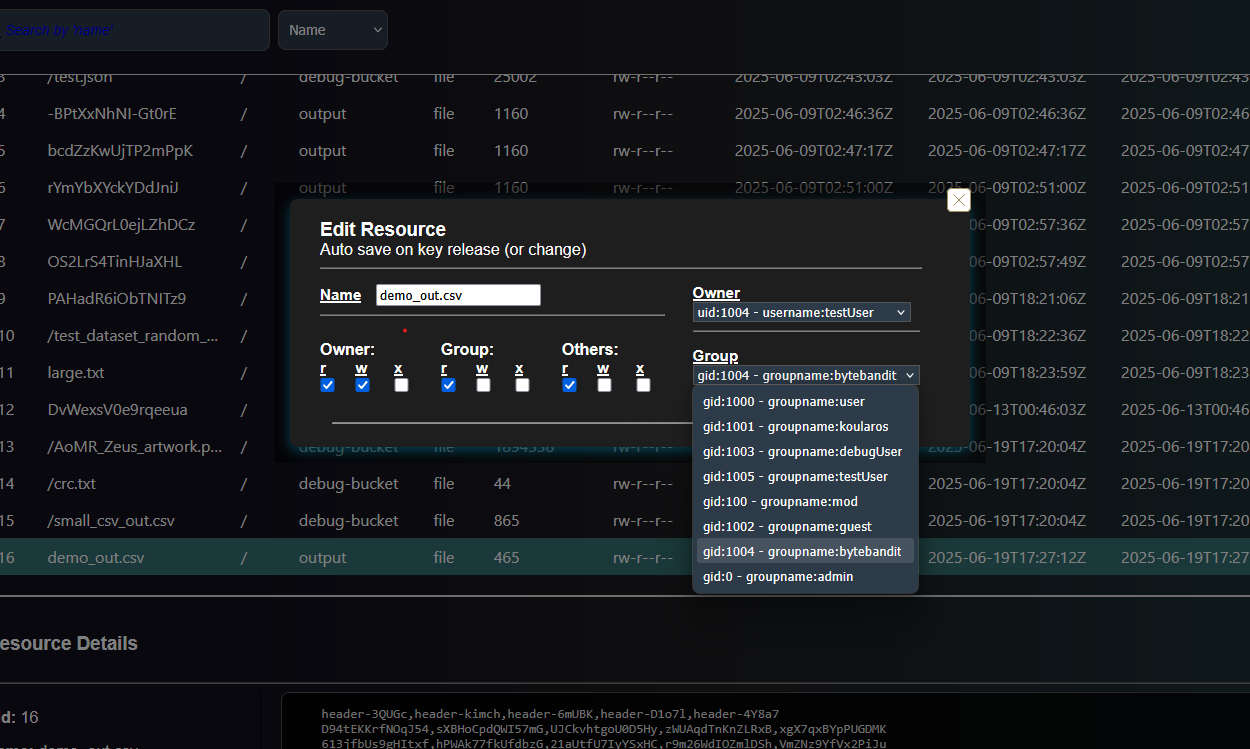
\includegraphics[width=\textwidth]{Images/kuspace_admin_EditResource.png}
        \caption{Edit Resource Metadata}
        \label{fig:admineditresource}
    \end{subfigure}
    \hfill
    \begin{subfigure}[b]{0.48\textwidth}
        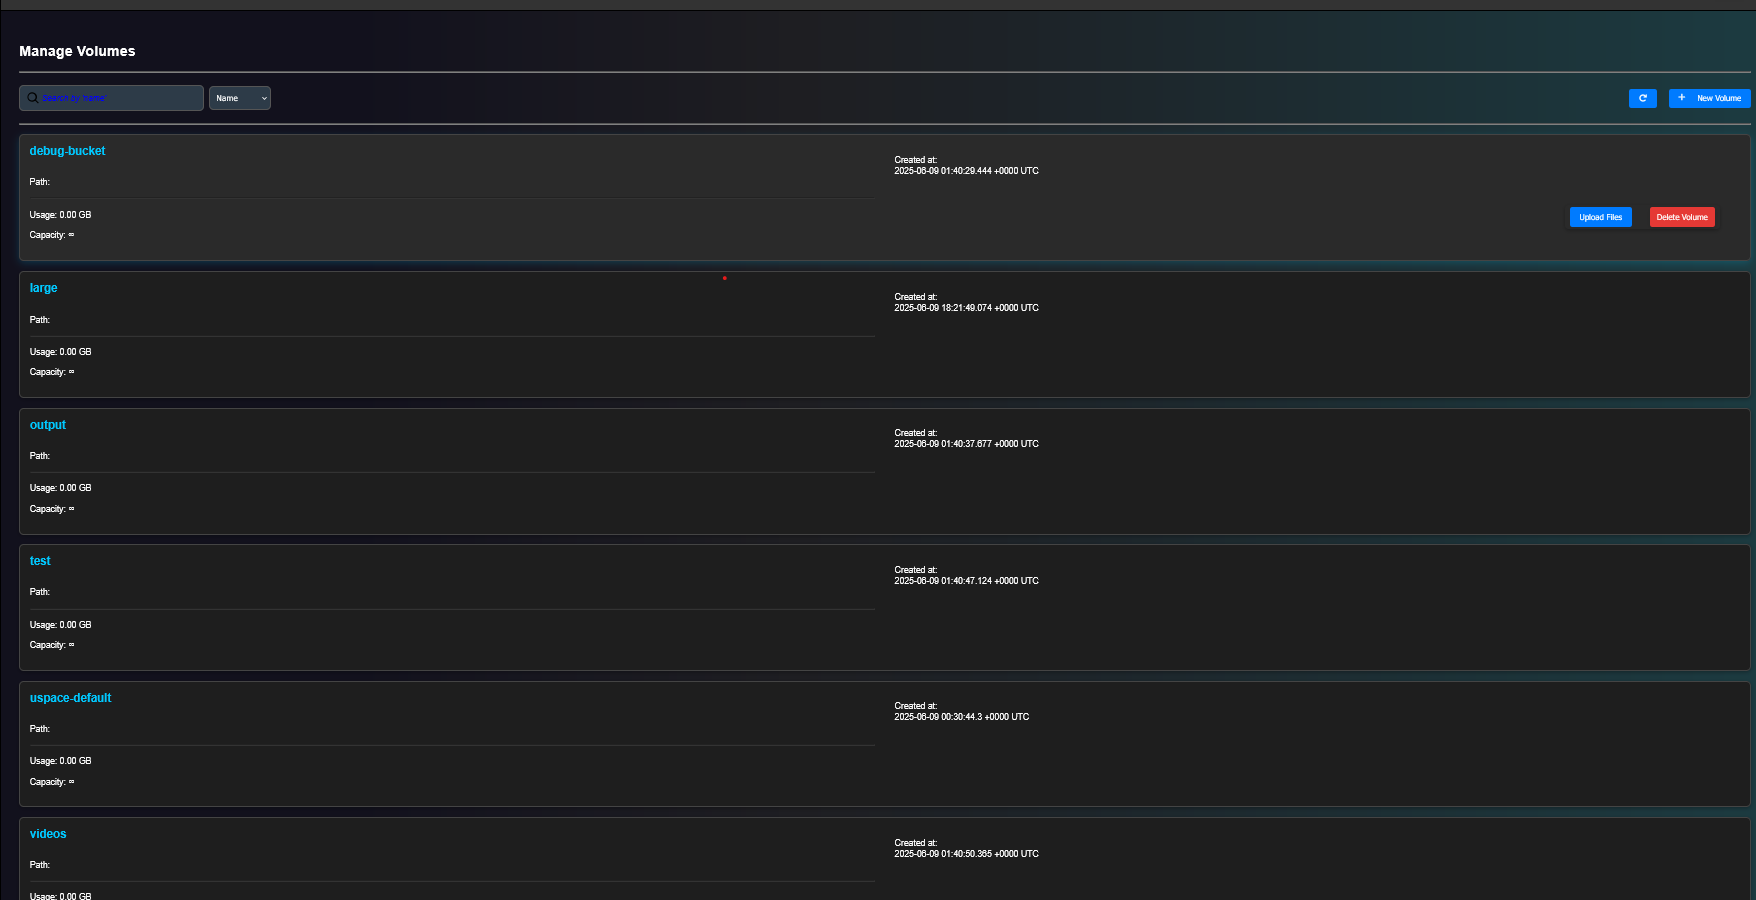
\includegraphics[width=\textwidth]{Images/kuspace_admin_ManageVolumes.png}
        \caption{Volume Overview}
        \label{fig:adminmanagevolumes}
    \end{subfigure}

    \vspace{1em}

    \begin{subfigure}[b]{0.48\textwidth}
        \includegraphics[width=\textwidth]{Images/kuspace_admin_CreateVolume.png}
        \caption{Create New Volume}
        \label{fig:admincreatevolume}
    \end{subfigure}
    \hfill
    \begin{subfigure}[b]{0.48\textwidth}
        \includegraphics[width=\textwidth]{Images/kuspace_admin_ManageJobs.png}
        \caption{Manage Jobs}
        \label{fig:adminmanagejobs}
    \end{subfigure}

    \vspace{1em}

    \centering
    \begin{subfigure}[b]{0.48\textwidth}
        \includegraphics[width=\textwidth]{Images/kuspace_admin_ModifyJob.png}
        \caption{Modify Submitted Job}
        \label{fig:adminmodifyjob}
    \end{subfigure}
    \hfill
    \begin{subfigure}[b]{0.48\textwidth}
        \includegraphics[width=\textwidth]{Images/kuspace_admin_Settings.png}
        \caption{Settings Panel}
        \label{fig:adminsettings}
    \end{subfigure}
    \caption{Kuspace admin views for storage and job management.}
\end{figure}
\vspace{0.5em}
\noindent


\newpage
\subsection{Job Examples}

In this section, we demonstrate two distinct job examples that showcase the system's ability to execute containerized applications over uploaded data:

\begin{itemize}
    \item A \textbf{Bash-based job} that counts the number of occurrences of the string \texttt{"bash"} within a 4GB file of random characters.
    \item A \textbf{DuckDB-based job} that computes a histogram of the first character of each line in a structured text file.
\end{itemize}

\subsubsection*{Example 1: Bash Job – Count Occurrences}

The input file consists of 4GB of random characters including the word \texttt{"bash"} scattered throughout.

\paragraph{Job Logic:}
\begin{verbatim}
grep -o 'bash' input.txt | wc -l
\end{verbatim}

\paragraph{Result:}  
\texttt{254} occurrences of \texttt{"bash"} were found.

This result can be verified locally using a terminal or text editor (assuming sufficient memory).

\begin{figure}[!htbp]
    \centering
    \begin{subfigure}[b]{0.9\textwidth}
        \includegraphics[width=\textwidth]{Images/bash_count_example.txt.png}
        \caption{Bash App job logic submitted via UI}
        \label{fig:examplebash1.1}
    \end{subfigure}

    \vspace{1em}

    \begin{subfigure}[b]{0.9\textwidth}
        \includegraphics[width=\textwidth]{Images/bash_count_result.png}
        \caption{Bash App job output}
        \label{fig:examplebash1.2}
    \end{subfigure}

    \vspace{1em}

    \begin{subfigure}[b]{0.9\textwidth}
        \includegraphics[width=\textwidth]{Images/bash_count.txt.png}
        \caption{Manual result verification (e.g., via editor)}
        \label{fig:examplebash1.3}
    \end{subfigure}
    \caption{Bash job: Counting occurrences of a word in a large file}
\end{figure}

\newpage
\subsubsection*{Example 2: DuckDB Job – Line Start Histogram}

This job uses a smaller text file to illustrate SQL capabilities more clearly. Each line in the file starts with a capital letter forming the line:

\begin{quote}
\texttt{DUCKDBBASHOCTAVE}
\end{quote}

\paragraph{Job Logic:}
\begin{verbatim}
CREATE TABLE lines AS SELECT * FROM {input};

SELECT substr(column0, 1, 1) AS first_char, count(*) AS line_count
FROM lines
GROUP BY first_char
ORDER BY line_count DESC;
\end{verbatim}

\paragraph{Result:}

\begin{verbatim}
D,2
C,2
B,2
A,2
U,1
K,1
S,1
H,1
O,1
T,1
V,1
E,1
\end{verbatim}

As expected, each starting letter is counted accurately and returned in descending order of frequency.

\begin{figure}[!htbp]
    \centering
    \begin{subfigure}[b]{0.9\textwidth}
        \includegraphics[width=\textwidth]{Images/duckdb_histogram_demo.png}
        \caption{DuckDB job query and configuration}
        \label{fig:exampleduckdb.1}
    \end{subfigure}

    \vspace{1em}

    \begin{subfigure}[b]{0.9\textwidth}
        \includegraphics[width=\textwidth]{Images/duckdb_histogram_demo_input.png}
        \caption{DuckDB job input file (preview)}
        \label{fig:exampleduckdb.2}
    \end{subfigure}

    \vspace{1em}

    \begin{subfigure}[b]{0.9\textwidth}
        \includegraphics[width=\textwidth]{Images/duckdb_histogram_demo_output.png}
        \caption{DuckDB job result}
        \label{fig:exampleduckdb.3}
    \end{subfigure}
    \caption{DuckDB job: Character frequency histogram from first line characters}
\end{figure}

\chapter{Evaluation and Robustness}
\label{Chapter-Evaluation-Robustness}

\section{Scalability Tests}

While no formal scalability benchmarks have been executed, the system design inherently supports horizontal scaling via Kubernetes. Each microservice is independently deployable and can be replicated or scaled depending on the workload.

Batch job execution is managed by Kubernetes Jobs, allowing multiple jobs to run concurrently, subject to resource constraints and cluster capacity. Storage and job queue sizes can be configured, and the system is prepared to integrate with scalable object storage solutions like MinIO or external S3-compatible services.

Future work may include stress-testing job submission rates, concurrent WebSocket connections, and storage read/write throughput.

\section{Security}

Authentication and authorization are enforced using JWT tokens issued by a dedicated service (Minioth) which are short-lived, and access control is modeled after a Unix-style permission system using FsLite. Sensitive inter-service communication is secured using a shared service secret.

The system properly distinguishes between user and admin roles, enforces ownership and group permissions on data access, and guards access to privileged routes. However, a formal security audit has not been conducted. Future improvements could include:

\begin{itemize}
    \item Rate limiting and brute-force protection.
    \item Improved logging and audit trails.
    \item Formal threat modeling and penetration testing.
\end{itemize}

\section{Fault Tolerance}

Fault tolerance is largely delegated to the Kubernetes runtime, which automatically restarts failed pods, monitors service health, and maintains declared desired state.

Jobs are submitted through an internal queue system and executed as isolated Kubernetes jobs. Failures in job execution do not compromise the stability of the core system; failed jobs are logged and reported via status messages.

Non-critical services such as the WebSocket server are loosely coupled and can be restarted independently without affecting core operations.

\section{Resource Usage}

Resource consumption is dynamic and depends on job definitions. Users may configure CPU, memory, and ephemeral storage requirements per job. After completion, jobs are deleted by Kubernetes, reducing runtime overhead. Metadata about jobs, volumes, and users is persistently stored in embedded databases (e.g., DuckDB, SQLite), which may grow over time but remain manageable.

Currently, no automatic cleanup of job metadata or disk quotas is enforced. Persistent logs are written to stdout and can be aggregated using external tools if deployed in production. Future work may explore:

\begin{itemize}
    \item Periodic pruning of old metadata and logs.
    \item Integration with resource monitoring dashboards (e.g., Grafana).
    \item Quota enforcement for user volume usage and job submissions.
\end{itemize}

\chapter{Conclusions and Future Work}
\label{Chapter-Conclusions}

\section{Conclusions}

This thesis presented the design and development of a modular, microservice-oriented job execution system tailored for Kubernetes-based infrastructures. Through a combination of lightweight services, clearly defined APIs, and a user-focused frontend, the platform enables authenticated users to upload data, submit analytical jobs, and retrieve results in a secure and controlled environment.

The system was implemented entirely in Go, using technologies such as Gin for HTTP routing, MinIO for object storage, and Kubernetes for orchestrated execution. A pluggable job architecture and storage abstraction layer allow for flexibility and future adaptability. Even though a formal evaluation was not conducted, the system demonstrates real-world viability through functional integration and local deployments on Minikube and Docker Desktop.

\section{Future Work}

Despite its completeness as a prototype, several areas of the system lend themselves to meaningful expansion and improvement:

\begin{itemize}
    \item \textbf{Caching and Optimization:} Introducing caching mechanisms (e.g., Redis) could reduce redundant computations and disk I/O, improving performance for repeated access to commonly used files or job results.
    
    \item \textbf{Job Pipelines:} Extending the job model to support pipelined execution—where the output of one tool feeds directly into another—would allow users to build more complex analytical workflows natively within the platform.
    
    \item \textbf{Distributed Job Models:} More sophisticated orchestration strategies could be explored, enabling distributed and cooperative execution of job chains, possibly integrating with task queues or event-driven architectures like Kafka or NATS.
    
    \item \textbf{Application Generation Framework:} A meta-application that allows administrators or advanced users to define new containerized applications (with their input/output schema and logic) via a UI or DSL would significantly expand the platform’s usability and extensibility.
    
    \item \textbf{CLI Client Tool:} To complement the web-based frontend, a command-line interface (CLI) tool could be developed, enabling power users and automation scripts to interact with the system more efficiently.
    
    \item \textbf{Evaluation and Benchmarking:} A structured performance and scalability analysis remains an open task. Real-cluster deployments and load testing would help validate assumptions about the system’s robustness and identify further bottlenecks.
\end{itemize}

In conclusion, the system serves as a strong foundation for scalable, secure, and user-friendly batch processing on Kubernetes. The outlined future work suggests a wide potential for transforming it into a general-purpose analytical platform adaptable across domains.


%----------------------------------------------------------------------------------------
%	THESIS CONTENT - APPENDICES
%----------------------------------------------------------------------------------------

\appendix % Cue to tell LaTeX that the following "chapters" are Appendices

% Include the appendices of the thesis as separate files from the Appendices folder
% Uncomment the lines as you write the Appendices

% Todo: comment out if not needed
% % Appendix A

\chapter{Frequently Asked Questions} % Main appendix title

\label{AppendixA} % For referencing this appendix elsewhere, use \ref{AppendixA}

\section{How do I change the colors of links?}

The color of links can be changed to your liking using:

{\small\verb!\hypersetup{urlcolor=red}!}, or

{\small\verb!\hypersetup{citecolor=green}!}, or

{\small\verb!\hypersetup{allcolor=blue}!}.

\noindent If you want to completely hide the links, you can use:

{\small\verb!\hypersetup{allcolors=.}!}, or even better: 

{\small\verb!\hypersetup{hidelinks}!}.

\noindent If you want to have obvious links in the PDF but not the printed text, use:

{\small\verb!\hypersetup{colorlinks=false}!}.

\chapter*{Appendix: Source Code Access}
The full source code of the project, including the backend services, FrontApp UI, and deployment configurations, can be found at:

\url{https://github.com/kyri56xcaesar/kuspace}

% \include{Appendices/AppendixC}

%----------------------------------------------------------------------------------------
%	BIBLIOGRAPHY
%----------------------------------------------------------------------------------------

\cleardoublepage\phantomsection\addcontentsline{toc}{chapter}{References}
\printbibliography[keyword={references}, title={References}]
\printbibliography[keyword={link}, title={External Links}]

%----------------------------------------------------------------------------------------

\end{document}